\documentclass{article}


% if you need to pass options to natbib, use, e.g.:
%     \PassOptionsToPackage{numbers, compress}{natbib}
% before loading neurips_2024


% ready for submission
\usepackage[final]{neurips_2024}


% to compile a preprint version, e.g., for submission to arXiv, add add the
% [preprint] option:
%     \usepackage[preprint]{neurips_2024}


% to compile a camera-ready version, add the [final] option, e.g.:
%     \usepackage[final]{neurips_2024}


% to avoid loading the natbib package, add option nonatbib:
%    \usepackage[nonatbib]{neurips_2024}


\usepackage[utf8]{inputenc} % allow utf-8 input
\usepackage[T1]{fontenc}    % use 8-bit T1 fonts
\usepackage{hyperref}       % hyperlinks
\usepackage{url}            % simple URL typesetting
\usepackage{booktabs}       % professional-quality tables
\usepackage{amsfonts}       % blackboard math symbols
\usepackage{nicefrac}       % compact symbols for 1/2, etc.
\usepackage{microtype}      % microtypography
\usepackage{xcolor}         % colors
\usepackage{amsmath}
\usepackage{amssymb}
\usepackage{mathtools}
\usepackage{amsthm}
\usepackage{caption}
\usepackage{subcaption}
\usepackage{wrapfig}
\usepackage[capitalize,noabbrev]{cleveref}

\title{Shapes analysis for time series.}


% The \author macro works with any number of authors. There are two commands
% used to separate the names and addresses of multiple authors: \And and \AND.
%
% Using \And between authors leaves it to LaTeX to determine where to break the
% lines. Using \AND forces a line break at that point. So, if LaTeX puts 3 of 4
% authors names on the first line, and the last on the second line, try using
% \AND instead of \And before the third author name.


\author{%
  Thibaut Germain \thanks{Corresponding author. Contact at \texttt{thibaut.germain@ens-paris-saclay.fr}} \\
  Centre Borelli, ENS Paris-Saclay\\
  4 av. des sciences, 91190 \\
  %\texttt{thibaut.germain@ens-paris-saclay.fr} \\
  % examples of more authors
  \And
  Samuel Gruffaz \\
  Centre Borelli, ENS Paris-Saclay\\
  4 av. des sciences, 91190 \\
  % Address \\
  %\texttt{samuel.gruffaz@ens-paris-saclay.fr} \\
  \AND
  Charles Truong \\
  Centre Borelli, ENS Paris-Saclay\\
  4 av. des sciences, 91190 \\
  %\texttt{charles.truong@ens-paris-saclay.fr} \\
  \And
  Laurent Oudre \\
  Centre Borelli, ENS Paris-Saclay\\
  4 av. des sciences, 91190 \\
  \And
  Alain Durmus \\
  CMAP, CNRS, Ecole polytechnique\\
  Institut Polytechnique de Paris\\
  91120 Palaiseau, France \\
}
% ready for submission
\usepackage[utf8]{inputenc} % allow utf-8 input
\usepackage[T1]{fontenc}    % use 8-bit T1 fonts

\usepackage{wrapfig,lipsum,booktabs}

%\usepackage{comment}

\usepackage{paralist}
\usepackage{booktabs}       % professional-quality tables
\usepackage{nicefrac}       % compact symbols for 1/2, etc.
\usepackage{multirow}
 \usepackage{xargs}

%\usepackage[tbtags]{amsmath}
%\usepackage{amsthm}
%\usepackage{bm}
\allowdisplaybreaks
\usepackage{amssymb,mathrsfs}
\usepackage{amsfonts}
\usepackage{mathtools}
\usepackage{upgreek}
\usepackage{graphicx}
\usepackage{wrapfig}
%\usepackage[dvipsnames]{xcolor}
\usepackage{soul}
\usepackage{pifont}
\usepackage{bbm}
%\usepackage[colorlinks = true, citecolor = black]{hyperref}
%\usepackage{algpseudocode,algorithm,algorithmicx}
\usepackage{stmaryrd}
\usepackage{array}
\usepackage{enumitem}
\def\UrlBreaks{\do\/\do-}
\usepackage{tikz}
\usepackage{pgfplots}
\usepackage{aliascnt}
\usepackage{todonotes}
\usepackage{cleveref}
\let\etoolboxforlistloop\forlistloop % save the good meaning of \forlistloop
\usepackage{autonum}
\let\forlistloop\etoolboxforlistloop % restore the good meaning of \forlistloop
\usepackage{bm}

\usepackage{accents}

\newcommand{\cmark}{\textcolor{green!80!black}{\ding{51}}}
\newcommand{\xmark}{\textcolor{red}{\ding{55}}}

\newcommand\barbelow[1]{%
  \underaccent{\bar}{#1}}

  %% Maxime' comments 
\definecolor{lightred}{rgb}{1, 0.8, 0.8}
\DeclareRobustCommand{\maxime}[1]{
{
    \begingroup
    \sethlcolor{lightred}
    \hl{(Maxime:) #1}
    \endgroup} 
}
\DeclareMathAlphabet{\mathpzc}{OT1}{pzc}{m}{it}
\theoremstyle{plain}
\makeatletter
\newtheorem{theorem}{Theorem}
\crefname{theorem}{theorem}{Theorems}
\Crefname{Theorem}{Theorem}{Theorems}


%\newtheorem*{lemma_nonumber*}{Lemma}


%\newaliascnt{lemma}{theorem}
\newtheorem{lemma}{Lemma}
%\aliascntresetthe{lemma}
%\crefname{lemma}{lemma}{lemmas}
%\Crefname{Lemma}{Lemma}{Lemmas}



\newaliascnt{corollary}{theorem}
\newtheorem{corollary}[corollary]{Corollary}
\aliascntresetthe{corollary}
\crefname{corollary}{corollary}{corollaries}
\Crefname{Corollary}{Corollary}{Corollaries}

\newaliascnt{proposition}{theorem}
\newtheorem{proposition}[proposition]{Proposition}
\aliascntresetthe{proposition}
\crefname{proposition}{proposition}{propositions}
\Crefname{Proposition}{Proposition}{Propositions}

\newaliascnt{definition}{theorem}
\newtheorem{definition}[definition]{Definition}
\aliascntresetthe{definition}
\crefname{definition}{definition}{definitions}
\Crefname{Definition}{Definition}{Definitions}

\newaliascnt{remark}{theorem}
\newtheorem{remark}[remark]{Remark}
\aliascntresetthe{remark}
\crefname{remark}{remark}{remarks}
\Crefname{Remark}{Remark}{Remarks}


\newtheorem{example}[theorem]{Example}
\crefname{example}{example}{examples}
\Crefname{Example}{Example}{Examples}


\crefname{figure}{figure}{figures}
\Crefname{Figure}{Figure}{Figures}

\newtheorem{assumption}{\textbf{H}\hspace{-3pt}}
\crefformat{assumption}{{\textbf{H}}#2#1#3}
\newtheorem{assumptionsup}{\textbf{A}\hspace{-3pt}}
\crefformat{assumptionsup}{{\textbf{A}}#2#1#3}
\newtheorem{assumptionnona}{\textbf{N}\hspace{-3pt}}
\crefformat{assumptionnona}{{\textbf{N}}#2#1#3}

\newtheorem{assumptionnonsup}{\textbf{M}\hspace{-3pt}}
\crefformat{assumptionnonsup}{{\textbf{M}}#2#1#3}

\def\rmM{\mathrm{M}}
\def\msf{\mathsf{G}}
\def\borel{\mathcal{B}}
\def\Qker{\mathrm{Q}}
\def\Rker{\mathrm{R}}
\def\Sker{\mathrm{S}}
\def\Pens{\mathscr{P}}
\def\Ltt{\mathtt{L}}
\def\Mtt{\mathtt{M}}
\def\Jac{\mathrm{Jac}}
\def\dom{\mathrm{dom}}
\def\msd{\mathsf{D}}
\def\msw{\mathsf{W}}
\newcommand{\rref}[1]{\textup{\Cref{#1}}}
\def\rmA{\mathrm{A}}
\def\rmB{\mathrm{B}}
\def\msu{\mathsf{U}}
\newcommand{\maxence}[1]{\todo[inline,color=green!40]{{\bf Maxence:~}#1}}
\newcommand{\valentin}[1]{\todo[inline,color=green!40]{{\bf Valentin:~}#1}}
%\newcommand{\alain}[1]{\todo[inline,color=green!40]{{\bf Alain:~}#1}}

% MACROS
% \newcommand{\w}{\mathbf{w}}
% \newcommand{\x}{\mathbf{x}}
% \newcommand{\y}{\mathbf{y}}
% \newcommand{\J}{\mathbf{J}}
% \newcommand{\f}{\mathbf{f}}
%\newcommand{\R}{\mathbb{R}}
\newcommand{\Image}{\text{Im}}
\newcommand{\Ker}{\text{Ker}}
\newcommand{\TM}{\Pi^\star\msm}
\newcommand{\Th}{\mathrm{S}_{h/2}}
\newcommand{\Rh}{\mathrm{R}_{h}}
\newcommand{\Gh}{\mathrm{G}_{h}}
\newcommand{\ug}{\underline{\mathrm{g}}}
\newcommand{\oGh}{\overline{\mathrm{G}_{h}}}
\newcommand{\uGh}{\underline{\mathrm{G}_{h}}}
\newcommand{\ugh}{\underline{\mathrm{g}_{h}}}
\newcommand{\ughz}{\underline{\mathrm{g}_{h,z}}}
\newcommand{\Fh}{\mathrm{F}_{h}}
\newcommand{\tildeFh}{\tilde{\mathrm{F}}_{h}}
\newcommand{\tildeGh}{\tilde{\mathrm{G}}_{h}}
\newcommand{\In}{\text{I}_n}
\newcommand{\phiRh}{\mathrm{R}_{h}^{\Phi}}
\newcommand{\tildeRh}{\tilde{\mathrm{R}}_{h}}
\newcommand{\Tminush}{\Pi_{-h/2}}
\newcommand*{\myotop}{\perp\mkern-20.7mu\bigcirc}
\newcommand{\TMx}[1]{\Pi^\star_{#1}\msm}


\newcommand{\tcmb}[1]{\textcolor{blue}{#1}}
\newcommand{\tcmo}[1]{\textcolor{orange}{#1}}
\newcommand{\tcmv}[1]{\textcolor{darkgreen}{#1}}


\def\M{\msm}
\def\vol{\text{vol}}

%%% Alain


%%% mathsf
\def\complementary{\mathrm{c}}
\def\msi{\mathsf{I}}
\def\msj{\mathsf{J}}
\def\msa{\mathsf{A}}
%\def\msd{\mathsf{X}}
\def\msdd{\mathsf{D}}
\def\msk{\mathsf{K}}
\def\msK{\mathsf{K}}
\def\msks{\mathsf{K}^{\star}}
\def\mss{\mathsf{S}}
\def\msn{\mathsf{N}}
\def\msat{\tilde{\mathsf{A}}}
\def\tgamma{\tilde{\gamma}}
\def\msb{\mathsf{B}} 
\def\msc{\mathsf{C}}
\def\mse{\mathsf{E}}
\def\msf{\mathsf{F}}
\def\mso{\mathsf{O}}
\def\msg{\mathsf{G}}
\def\msh{\mathsf{H}}
\def\bmsh{\bar{\msh}}
\def\msm{\mathsf{M}}
\def\msu{\mathsf{U}}
\def\msv{\mathsf{V}}
\def\msr{\mathsf{R}}
\newcommand{\msff}[2]{\mathsf{F}_{#1}^{#2}}
\def\msp{\mathsf{P}}
\def\msq{\mathsf{Q}}
\def\msx{\mathsf{X}}
\def\msz{\mathsf{Z}}
\def\msy{\mathsf{Y}}



%% mathcal
\def\mca{\mathcal{A}}
\def\bmca{\bar{\mathcal{A}}}
\def\mcd{\mathcal{D}}
\def\mcl{\mathcal{L}}
\def\mcs{\mathcal{S}}
\def\mct{\mathcal{T}}
\def\tmct{\tilde{\mathcal{T}}}
\def\tmcs{\tilde{\mathcal{S}}}
\def\bmcl{\bar{\mathcal{L}}}
\def\bmcs{\bar{\mathcal{S}}}
\def\bmct{\bar{\mathcal{T}}}
\def\mcat{\tilde{\mathcal{A}}}
\def\mcab{\bar{\mathcal{A}}}
\def\mcbb{\mathcal{B}}  %%% \mcb est déjà pris
\newcommand{\mcb}[1]{\mathcal{B}(#1)}
\def\mcc{\mathcal{C}}
\def\mcy{\mathcal{Y}}
\def\mcx{\mathcal{X}}
\def\mce{\mathcal{E}}
\def\mcf{\mathcal{F}}
\def\mcg{\mathcal{G}}
\def\mch{\mathcal{H}}
\def\mcm{\mathcal{M}}
\def\mcu{\mathcal{U}}
\def\mcv{\mathcal{V}}
\def\mcr{\mathcal{R}}
\def\tmcr{\tilde{\mathcal{R}}}
\newcommand{\mcff}[2]{\mathcal{F}_{#1}^{#2}}
\def\mcfb{\bar{\mathcal{F}}}
\def\bmcf{\bar{\mathcal{F}}}
\def\mcft{\tilde{\mathcal{F}}}
\def\tmcf{\tilde{\mathcal{F}}}
\def\mcp{\mathcal{P}}
\def\mcq{\mathcal{Q}}
\def\mcz{\mathcal{Z}}

%% mathbb

\def\rset{\mathbb{R}}
\def\mE{\mathbb{E}}
\def\rsets{\mathbb{R}^*}
\def\cset{\mathbb{C}}
\def\zset{\mathbb{Z}}
\def\nset{\mathbb{N}}
\def\nsets{\mathbb{N}^*}
\def\qset{\mathbb{Q}}
\def\Rset{\mathbb{R}}
\def\Cset{\mathbb{C}}
\def\Zset{\mathbb{Z}}
\def\Nset{\mathbb{N}}
\def\Tset{\mathbb{T}}


%%%% mathrm 
\def\rmm{\mathrm{m}}
\def\Rsetm{\mathrm{m}}
\def\rmd{\mathrm{d}}
\def\Rsetd{\mathrm{d}}
\def\rmf{\mathrm{f}}
\def\Rsetl{\mathrm{L}}
\def\RsetH{\mathrm{H}}
\def\rmH{\mathrm{H}}
\def\rml{\mathrm{L}}
\def\Rsete{\mathrm{e}}
\def\rme{\mathrm{e}}
\def\rmn{\mathrm{n}}
\def\Rsetn{\mathrm{n}}
\def\RsetC{\mathrm{C}}
\def\RsetCb{\mathrm{C}_{\operatorname{b}}}
\def\rmCb{\mathrm{C}_{\operatorname{b}}}
\def\Rsetc{\mathrm{c}}
\def\rmc{\mathrm{c}}
\def\rmC{\mathrm{C}}
\def\rma{\mathrm{a}}
\def\Rseta{\mathrm{a}}
\def\rmU{\mathrm{U}}
\def\rmY{\mathrm{Y}}
\def\rmb{\mathrm{b}}

%%%% mathfrak
\def\frX{\mathfrak{X}}
\def\frg{\mathfrak{g}}


% Operands
\newcommand{\absolute}[1]{\left\vert #1 \right\vert}
\newcommand{\abs}[1]{\left\vert #1 \right\vert}
\newcommand{\absLigne}[1]{\vert #1 \vert}
\newcommand{\tvnorm}[1]{\| #1 \|_{\mathrm{TV}}}
\newcommand{\tvnormEq}[1]{\left \| #1 \right \|_{\mathrm{TV}}}
\newcommand{\Vnorm}[2][1=V]{\| #2 \|_{#1}}
\newcommand{\normpi}[2][2=\Rsetl^2(\pi)]{\left\Vert  #1 \right\Vert_{#2}}
\newcommand{\normH}[2][2=2]{\left\Vert  #1 \right\Vert}
\newcommand{\normHLigne}[2][2=2]{\Vert  #1 \Vert}
\newcommand{\normHLine}[2][2=2]{\Vert  #1 \Vert}
\newcommand{\normmu}[2][2=2]{\left\Vert  #1 \right\Vert_{#2}}
\newcommand{\normopmu}[2][2=2]{\left\vvvert  #1 \right\vvvert_{#2}}
\newcommand{\normoppi}[2][2=\rml^2(\pi)]{\left\vvvert  #1 \right\vvvert_{#2}}
\newcommand{\normopH}[2][2=2]{\left\vvvert  #1 \right\vvvert}
\newcommand{\normop}[2][2=2]{\left\vvvert  #1 \right\vvvert}
\newcommandx{\psr}[3][3=]{\left\langle#1,#2 \right\rangle_{#3}}
\newcommandx{\normr}[2][2=]{ \left\Vert#1 \right\Vert_{#2}}
\newcommandx{\psrLigne}[3][3=]{\langle#1,#2 \rangle_{#3}}
\newcommandx{\normrLigne}[2][2=]{ \Vert#1 \Vert_{#2}}
\newcommand{\pspi}[2]{\left\langle#1,#2 \right\rangle_2}
\newcommand{\psH}[2]{\left\langle#1,#2 \right\rangle}
\newcommand{\psmu}[2]{\left\langle#1,#2 \right\rangle_2}
\newcommand{\psmuLigne}[2]{\langle#1,#2 \rangle_2}
\newcommand{\normpiLine}[2][2=2]{\Vert  #1 \Vert_{#2}}
\newcommand{\normpiLigne}[2][2=2]{\Vert  #1 \Vert_{#2}}
\newcommand{\normmuLine}[2][2=2]{\Vert  #1 \Vert_{#2}}
\newcommand{\normmuLigne}[2][2=2]{\Vert  #1 \Vert_{#2}}
\newcommand{\normopmuLine}[2][2=2]{\vvvert  #1 \vvvert_{#2}}
\newcommand{\normopmuL}[2][2=2]{\normopmuLine{#1}[#2]}
\newcommand{\normopHLine}[2][2=2]{\vvvert  #1 \vvvert}
\newcommand{\normopLine}[2][2=2]{\vvvert  #1 \vvvert}
\newcommand{\pspiLine}[2]{\langle#1,#2 \rangle_2}
\newcommand{\psmuLine}[2]{\langle#1,#2 \rangle_2}
\newcommand{\VnormEq}[2][1=V]{\left\| #2 \right\|_{#1}}
\newcommandx{\norm}[2][1=]{\ifthenelse{\equal{#1}{}}{\left\Vert #2 \right\Vert}{\left\Vert #2 \right\Vert^{#1}}}
\newcommand{\normLigne}[1]{\| #1 \|}
\newcommand{\crochet}[1]{\left\langle#1 \right\rangle}
\newcommand{\parenthese}[1]{\left(#1 \right)}
\newcommand{\parentheseLigne}[1]{(#1 )}
\newcommand{\parentheseDeux}[1]{\left[ #1 \right]}
\newcommand{\parentheseDeuxLigne}[1]{[ #1 ]}
\newcommand{\defEns}[1]{\left\lbrace #1 \right\rbrace }
\newcommand{\defEnsLigne}[1]{\lbrace #1 \rbrace }
\newcommand{\defEnsPoint}[1]{\left\lbrace #1 \right. }
\newcommand{\defEnsPointDeux}[1]{\left. #1 \right  \rbrace }
\newcommand{\defEnsL}[1]{\left\lbrace #1 \right. }
\newcommand{\defEnsR}[1]{\left. #1 \right  \rbrace }

% Proba
\newcommand{\proba}[1]{\mathbb{P}\left( #1 \right)}
\newcommand{\PP}{\mathbb{P}}
\newcommand{\probaLigne}[1]{\mathbb{P}( #1 )}
\newcommand\probaMarkovTilde[2][2=]
{\ifthenelse{\equal{#2}{}}{{\widetilde{\mathbb{P}}_{#1}}}{\widetilde{\mathbb{P}}_{#1}\left[ #2\right]}}
\newcommand{\probaMarkov}[2]{\mathbb{P}_{#1}\left( #2\right)}
\newcommand{\PE}{\bbE} %j'ai l'impression qu'il manquait ça
\newcommand{\expe}[1]{\PE \left[ #1 \right]}
\newcommand{\expeExpo}[2]{\PE^{#1} \left[ #2 \right]}
\newcommand{\expeLigne}[1]{\PE [ #1 ]}
\newcommand{\expeLine}[1]{\PE [ #1 ]}
\newcommand{\expeMarkov}[2]{\PE_{#1} \left[ #2 \right]}
\newcommand{\expeMarkovLigne}[2]{\PE_{#1} [ #2 ]}
\newcommand{\expeMarkovExpo}[3]{\PE_{#1}^{#2} \left[ #3 \right]}
\newcommand{\probaMarkovTildeDeux}[2]{\widetilde{\mathbb{P}}_{#1} \left[ #2 \right]}
\newcommand{\expeMarkovTilde}[2]{\widetilde{\PE}_{#1} \left[ #2 \right]}


\newcommand{\plusinfty}{+\infty}
\def\ie{\textit{i.e.}}
\def\cadlag{càdlàg}
\def\eqsp{\;}
\def\eqand{\quad \text{  and  }\quad }
\renewcommand{\iint}[2]{\{ #1,\ldots,#2\}}
\newcommand{\coint}[1]{\left[#1\right)}
\newcommand{\ocint}[1]{\left(#1\right]}
\newcommand{\ooint}[1]{\left(#1\right)}
\newcommand{\ccint}[1]{\left[#1\right]}
\newcommand{\cointLigne}[1]{[#1)}
\newcommand{\ocintLigne}[1]{(#1]}
\newcommand{\oointLigne}[1]{(#1)}
\newcommand{\ccintLigne}[1]{[#1]}
\newcommand{\cointLine}[1]{[#1)}
\newcommand{\ocintLine}[1]{(#1]}
\newcommand{\oointLine}[1]{(#1)}
\newcommand{\ccintLine}[1]{[#1]}


\newcommand{\boule}[2]{\operatorname{B}(#1,#2)}
\newcommand{\ball}[2]{\operatorname{B}(#1,#2)}
\newcommand{\cball}[2]{\overline{\operatorname{B}}(#1,#2)}
\newcommand{\ballc}[2]{\operatorname{B}^\rmc(#1,#2)}
\newcommand{\boulefermee}[2]{\overline{\mathrm{B}}(#1,#2)}
\def\TV{\mathrm{TV}}
\newcommand\sequence[3][2=,3=]
{\ifthenelse{\equal{#3}{}}{\ensuremath{\{ #1_{#2}\}}}{\ensuremath{\{ #1_{#2}, \eqsp #2 \in #3 \}}}}
\newcommand\sequenceD[3][2=,3=]
{\ifthenelse{\equal{#3}{}}{\ensuremath{\{ #1_{#2}\}}}{\ensuremath{( #1)_{ #2 \in #3} }}}

\newcommand{\sequencen}[2][2=n\in\N]{\ensuremath{\{ #1_n, \eqsp #2 \}}}
\newcommand\sequenceDouble[4][3=,4=]
{\ifthenelse{\equal{#3}{}}{\ensuremath{\{ (#1_{#3},#2_{#3}) \}}}{\ensuremath{\{  (#1_{#3},#2_{#3}), \eqsp #3 \in #4 \}}}}
\newcommand{\sequencenDouble}[3][3=n\in\N]{\ensuremath{\{ (#1_{n},#2_{n}), \eqsp #3 \}}}


\newcommand{\wrt}{w.r.t.}
\newcommand{\Withoutlog}{w.l.o.g.}
\def\iid{i.i.d.}
\def\ifof{if and only if}
\def\eg{e.g.}
\def\Id{\mathrm{Id}}
\def\Idd{\mathrm{I}_d}
\newcommand{\ensemble}[2]{\left\{#1\,:\eqsp #2\right\}}
\newcommand{\ensembleLigne}[2]{\{#1\,:\eqsp #2\}}
%\newcommand{\set}[2]{\ensemble{#1}{#2}}
\def\rmD{\mathrm{D}}%%rmd déjà pris
\def\Rsetd{\mathrm{D}}


\def\Tr{\mathrm{Tr}}
\def\generator{\calL}
\newcommand{\core}{\rmc}
\def\lambdac{\lambda_{\mathrm{c}}}
\def\bfe{\mathbf{e}}

\newcommand{\alain}[1]{\todo[color=red!20]{{\textbf AL:} #1}}
 \newcommand{\alaini}[1]{\todo[color=red!20,inline]{{\textbf AL:} #1}}
  \newcommand{\pablo}[1]{\todo[color=black!20]{{\textbf PJ:} #1}}
   \newcommand{\pabloi}[1]{\todo[color=black!20,inline]{{\textbf PJ:} #1}}
 \def\a{a}
\def\domain{\mathrm{D}}
\def\card{\operatorname{card}}
\def\bigone{\operatorname{1}}
\def\bigO{\mathcal{O}}
\def\Cp{C_{\operatorname{P}}}
\def\core{\mathsf{C}}
\def\entropyA{\mathscr{H}}
\def\range{\operatorname{Ran}}
\def\kernel{\operatorname{Ker}}
\def\spec{\operatorname{Spec}}

%%%%%%%%%%%%
% function
\def\ff{f}
\def\gg{g}

\newcommand\overlineb[1]{{#1}}
\def\poly{\mathrm{poly}}
\def\veps{\varepsilon}
\def\trace{\operatorname{Tr}}
\def\sign{\operatorname{sgn}}
\def\diag{\operatorname{diag}}
\def\diam{\operatorname{diam}}
\newcommand\tcb[1]{\textcolor{cyan}{#1}}
\newcommand\tcbb[1]{\textcolor{blue}{#1}}
\newcommand\tcr[1]{\textcolor{red}{#1}}
\def\rateConv{\alpha}
\def\vareps{\varepsilon}
\def\sphere{\mathbb{S}}
\newcommand{\1}{\mathbbm{1}}


\newcommand{\vphi}{\varphi}
\newcommand{\even}{\mathrm{e}}

\def\restriction#1#2{\mathchoice
              {\setbox1\hbox{${\displaystyle #1}_{\scriptstyle #2}$}
              \restrictionaux{#1}{#2}}
              {\setbox1\hbox{${\textstyle #1}_{\scriptstyle #2}$}
              \restrictionaux{#1}{#2}}
              {\setbox1\hbox{${\scriptstyle #1}_{\scriptscriptstyle #2}$}
              \restrictionaux{#1}{#2}}
              {\setbox1\hbox{${\scriptscriptstyle #1}_{\scriptscriptstyle #2}$}
              \restrictionaux{#1}{#2}}}
\def\restrictionaux#1#2{{#1\,\smash{\vrule height .8\ht1 depth .85\dp1}}_{\,#2}}



%\DeclareMathOperator{\Var}{Var}

%%%%%%%%%%%%%%%%%%%%%%%%%%%%%%%%%%%%%%%%%%%%%%%%%%%%5
%%%%%% Pablo

\def\rmX{\mathrm{X}}
\def\rmVar{\mathrm{Var}}

\def\Ret{\mathrm{Ret}}

\def\bphi{\bar{\phi}}
\def\bgamma{\bar{\gamma}}

\def\loiGauss{\mathrm{N}}
\def\tx{\tilde{x}}
\def\tz{\tilde{z}}



\newcommand\norme[1]{\left\Vert #1 \right\Vert}


\def\parallelTransport{\Pi}
\def\distM{\mathrm{d}_{\msm}} %we prefer \Theta for the manifold
\def\distT{\rho_{\Theta}}
\def\metricM{\mathfrak{g}}
\def\vol{\mathrm{vol}}
\def\volM{\mathrm{vol}_{\msm}}
\def\grad{\mathrm{grad}\,}
\def\Hess{\mathrm{Hess}\,}
\def\teta{\tilde{\eta}}
\def\rmD{\mathrm{D}}

\def\noise{e}
\def\hnoise{\hat{e}}
\def\Exp{\mathrm{Exp}}
\def\Log{\mathrm{Log}}
\def\planT{\rmT}
\def\Cut{\mathrm{Cut}}
\def\ID{\mathrm{ID}}
\def\dupgamma{\dot{\upgamma}}


\def\grassmann{\mathrm{Gr}}
\def\stiefel{\mathrm{St}}
\def\transpose{\top}
\def\scrl{\mathscr{L}}
\def\scrlinf{\scrl_{\infty}}
\def\scrlU{\scrl^{(1)}}
\def\scrlD{\scrl^{(2)}}

\def\metric{\metricM}

\def\cu{\overline{c}}
\def\cl{\underline{c}}

\def\sigmaZ{\sigma_0^2}
\def\sigmaU{\sigma_1^2}
\def\bfb{\mathbf{b}}
\def\ttheta{\tilde{\theta}}
\def\Gammabf{\boldsymbol{\Gamma}}

\newcommand{\beq}{\begin{equation}}
\newcommand{\eeq}{\end{equation}}

%\def\bf1{\boldsymbol{1}}
\def\proj{\operatorname{proj}}
\def\Leb{\mathrm{Leb}}
\def\Vdist{V_2}
\def\VHuber{V_1}
\def\thetas{{\theta^{\star}}}
\def\thetaspi{{\theta^{\star}_{\pi}}}
\def\supp{\mathrm{supp}}
\def\constanteC{C}

\def\ConstH{C_H}
\def\rmcl{\mathrm{Cl}}
\def\vt{\mathpzc{V}}

%\renewcommand\hmmax{0}
%\renewcommand\bmmax{0}
\def\bnu{\bar{\nu}}
\def\bupeta{\bar{\upeta}}
\def\tb{\tilde{b}}
\def\cupeta{\check{\upeta}}
\def\gVar{g} %fonctº lisse sur la variété
\def\gPlan{\mathrm{g}} %fonctº lisse sur l'esp Tangent
\def\gInter{\mathpzc{g}} %fonctº lisse sur intervalle réel
\def\dz{\operatorname{dz}}
\def\argmin{\operatorname{argmin}}

\newcommand{\floor}[1]{\left\lfloor #1 \right\rfloor}
\newcommand{\ceil}[1]{\left\lceil #1 \right\rceil}
\def\btheta{\bar{\theta}}
\def\tsigma{\tilde{\sigma}}
\def\tf{\tilde{f}}
\def\MKer{Q_{\upeta}}
\def\bu{\bar{u}}

\def\planTsT{\planT_{\thetas}\Theta}
\def\bouletan{\bar{\mathbb{B}}}
\def\SPD{\mathrm{Sym}}


\newcommand*{\dd}{\mathop{}\!\mathrm{d}}
\def\ee{~}


%%%%%%%%%%%%%%%%%%%%%%%%%%
%%%  hmc notation
\def\orbit{\mathcal{O}}
\def\F{U}


\def\Psiverlet{\Psi}
\newcommandx{\gperthmc}[2][1=,2=]{\ifthenelse{\equal{#1}{}}{\Xi}{\ifthenelse{\equal{#2}{}}{\Xi_{h,#1}}{\Xi_{#2,#1}}}}
\newcommandx{\Phiverlet}[2][1=,2=]{\ifthenelse{\equal{#1}{}}{\Phi}{\Phi_{#1}^{\circ (#2)}}}
\newcommandx{\gpertub}[2][1=,2=]{\ifthenelse{\equal{#1}{}}{g}{g_{#1}^{#2}}}
\newcommandx{\Phiverletq}[2][1=,2=]{\ifthenelse{\equal{#1}{}}{\widetilde{\Phi}}{\widetilde{\Phi}_{#1}^{\circ (#2)}}}
\newcommandx{\Phiverletqi}[2][1=,2=]{\ifthenelse{\equal{#1}{}}{\bar{\Psi}}{\bar{\Psi}_{#1}^{(#2)}}}
\newcommandx{\Pkerhmc}[2][1=,2=]{\ifthenelse{\equal{#1}{}}{\mathrm{P}}{\mathrm{P}_{#1, #2}}}
\newcommandx{\tPkerhmc}[2][1=,2=]{\ifthenelse{\equal{#1}{}}{\tilde{\mathrm{P}}}{\tilde{\mathrm{P}}_{#1, #2}}}
\newcommandx{\PkerhmcD}[2][1=,2=]{\ifthenelse{\equal{#1}{}}{\mathrm{K}}{\mathrm{K}_{#1, #2}}}
\def\rmp{\mathrm{p}}
\def\rmq{\mathrm{q}}
\def\Kmax{K_{\mathrm{m}}}
\def\mcs{\mathcal{S}}
\def\gauss{\mathrm{N}}
\def\Kker{\mathrm{K}}
\def\Tker{\Pi}
\def\Mmatrix{M}
\def\argmax{\text{argmax}}
\newcommandx{\thetahat}[1][1=]{\ifthenelse{\equal{#1}{}}{\hat{\theta}}{\hat{\theta}(#1)}}
\newcommandx{\Kerpi}[2][1=,2=]{\ifthenelse{\equal{#1}{}}{\Pi}{\Pi_{#1}^{#2}}}
\newcommandx{\poinu}[2][1=,2=]{\ifthenelse{\equal{#1}{}}{\nu}{\nu_{#1}^{#2}}}
\def\lyapD{\mathpzc{V}}
\def\LyapD{\mathpzc{V}}
\def\VlyapD{\mathpzc{V}}
\def\lyapDs{\mathpzc{V}^*}
\def\LyapDs{\mathpzc{V}^*}
\def\VlyapDs{\mathpzc{V}^*}

\def\tsig{\tilde{s}}

%%%
% mathbf
\def\bfs{\mathbf{s}}



%%%%
% accro
\def\pos{\mathrm{pos}}
\def\dir{\mathrm{dir}}
\newcommand\sam[1]{\textcolor{blue}{#1}}
\newcommand\thi[1]{\textcolor{orange}{#1}}
\begin{document}


\maketitle
%In this paper we propose an unsupervised representation method (TS-LDDMM) to analyze inter-individual variability of time series dataset.
    %Inspired by the shape analysis literature, we extend Large Deformation Diffeomorphic Metric Mapping (LDDMM) to time series, considering the temporal evolution as their distinctive feature.  
    % Given a dataset of $N$ individual's time series $(s^j)_{j\in[N]}$,
    %  we learn a time series of reference $\mathbf{s}_0$ encoding the common part of the individuals as well as diffeomorphisms $(\phi^j)_{j\in[N]}$ encoding the specificities of each individual:
    %  $s^j$ is seen as the transformation of $\mathbf{s}_0$ by $\phi_j$.
    %  Then, the parameters $(\alpha_j)_{j\in[N]}$ encoding the diffeomorphisms $(\phi^j)_{j\in[N]}$ are used as the features representation related to each time series $s^j$.
    %At the crossroads between URL for time series and shape analysis. %the algorithm extends the Large Deformation Diffeomorphic Metric Mapping (LDDMM) to the case of time series. This extension is a nontrivial application of the LDDMM framework since it involves applying deformations to the graph of time series, which have more structure than curves due to the inclusion of the temporal dimension.

\begin{abstract}
Analyzing inter-individual variability of physiological functions is particularly appealing in medical and biological contexts to describe or quantify health conditions. Such analysis can be done by comparing individuals to a reference one with time series as biomedical data.
This paper introduces an unsupervised representation learning (URL) algorithm for time series tailored to inter-individual studies. The idea is to represent time series as deformations of a reference time series. The deformations are diffeomorphisms parameterized and learned by our method called TS-LDDMM. Once the deformations and the reference time series are learned, the vector representations of individual time series are given by the parametrization of their corresponding deformation. At the crossroads between URL for time series and shape analysis, the proposed algorithm handles irregularly sampled multivariate time series of variable lengths and provides shape-based representations of temporal data.
In this work, we establish a representation theorem for the graph of a time series and derive its consequences on the LDDMM framework. We showcase the advantages of our representation compared to existing methods using synthetic data and real-world examples motivated by biomedical applications.
\end{abstract}





% citep
% \section{TODO}
% %De ce que je comprends , les gens font surtout des variational auto encoder, ou du masking
% %Mentionner que la méthode proposé peut être utilisé avec des réseaux
% %\sam{Approche NTK, fédéré personalisation, projet avec Axel, Lien entre continuous normalizing flow}
% Plan intro: 
% \begin{itemize}
%     \item Representation of patterns in time series has several applications in biology, but halso for classification, deep learning finds features automaticly.
%      Taking or not taking into account time can be done with DTW. However, either the representation is the result of a black box and need post analysis to be understand,
%       which is difficult to apply statiscal tools on it, or the representation is desgned by hand to select relevant features, but the capacity of analysis is limited by the knowledge of the designer.
%      \item In shape analysis, representation of shapes for statistical analysis in a long time issue, which has been solved mainly by the LDDMM framework. Representing shapes as diffeomorpshims of a common shape. 
%      \item However, this tool has not been yet applied on time series, even if there is already some tools developped for oriented curves. 
%      \item In this work, we propose to apply LDDMM to time series and to show its interest to derive an interpretable and unsupervised representation of patterns in time series.
%      We proposed some tools developped in the shape analysis community to the researcher interested in machine learning and time series ones.
%      \item First, we introduce our assumptions regarding the dataset and the main problem of diffeomorpshim learning. Then, we show how to solve it with LDDMM .
%       We expose how to apply it to time series by selecting wisely a RKHS kernel, motivating it with a representation theorem.
%       experiments on synthetic data are presented to show that the parameter of representation are identifiable when the time seriess are not too sharp and the kernels parameter well tuned. 
%       Then, we sh-ow how to apply the method on an unsupervised case of moouse respeitaory dataset and a supervised one on ... .

% \end{itemize}

% One option to tackle this issue is to derive ...
% feature representation of time series which depends on the problem at hand.
% which is parti... -> which is of prime interest in ...

\section{Introduction}
%https://arxiv.org/abs/1811.00075
%Appliqué sur les "UWaveGestureLibrary","ArticularyWordRecognition","Cricket" pour l'archive UEA
%"ArrowHead", "BME", "ECG200","FacesUCR","GunPoint" dans le cas univarié

%Idée de parler d'inter individualité, spécialiser davantage
%k shape, shapelets , ye2009time
%\thi{à reformuler pour faire moins stupide}

%\sam{Aller droit au but, se servir de la section related works pour détailler, notamment enlever le premier paragraphe dire directement que l'on veut faire du unsupervised represnetation learning for time series mais en s'intéressant par ticulièrement à la notion de shape.
%Parler du contexte biomédical, définir la shape. Parler de shape analysis, introduire notre problème de représentation, dire que nous on propose une structure adapté aux time series.}

% In this paper, we propose an unsupervised representation learning method (URL) for time series \cite{trirat2024universal,meng2023unsupervised} by giving a special attention to their \textit{shapes} for studying inter-variability in biomedical applications.
% In particular, the method handle time series with \textbf{irregular sampling} and \textbf{different sizes}.
% This work belongs to the shape analysis literrature: %which focus on the statistical analysis of various mathematical objects invariant under rotations, dilations, or time parameterization.
%  we extend Large Deformation Diffeomorphic Metric Mapping (LDDMM) \cite{beg2005computing,vaillant2004statistics} to the case of time series data by applying difformations to their graph.
% However, time series graph have more structure than 1D curves:
%  a graph time series transformation by a general diffeomorphism is not always a graph time series.
% This work is at the crossroad of URL for time series and shape analysis; we hope it will benefit to both communities.
%A time series is a set of values indexed by time \cite{trirat2024universal}.
%This type of data is prevalent in biology and medicine for recording physiological time series , as well as in the broader context of the Internet of Things sensors \cite{fathy2018large} and measurements in physical systems \cite{luo2021deep}.
 %However, due to the nature of such data, which have different sample sizes and incorporate a temporal evolution, classical statistical analysis, and machine learning methods need refinement \cite{anderson2011statistical}.
 %One option to tackle this issue is to derive a feature representation of time series, which depends on the problem at hand \cite{trirat2024universal}.

Our goal is to analyze the inter-individual variability of a time series dataset, which is of prime interest in medicine and biology \cite{guscelli2019importance,wang2016research,bar2012studying,germain2023unsupervised}.
More specifically, we aim to find an unsupervised features representation method which encode the specificity of an individual compared to another. 
In physiology, studying the different \textit{shapes} in a time series related to biological phenomena and their variations according to individual or pathology is common.
However, a \textit{shape} has no clear definition; it is more an intuitive way to speak about the silhouette of a pattern in a time series. In this paper, we refer to as the shape of a time series, the graph of this signal.

Although a community structure with representatives can be learned in an unsupervised way \cite{trirat2024universal,meng2023unsupervised} using contrastive loss \cite{franceschi2019unsupervised,tonekaboni2021unsupervised,meng2023unsupervised} or similarity measures \cite{asgari2023clustering,germain2023unsupervised,paparrizos2015k,ye2009time},
studying the inter-individual variability of shapes within a cluster \cite{niennattrakul2007inaccuracies,shirato2023identifying} is still an open problem in URL.
     %In this paper, we aim to go beyond group structure by giving an unsupervised data-driven method that represents the specificity of each individual's shape \cite{vidal2021perceptual}.
  %For instance, the shape of a heartbeat in an Electrocardiogram (ECG) -the pattern- has been well studied \cite{madona2021pqrst} with the PQRST decomposition (see figure\sam{fill}).
  %There exist several methods to detect and segment patterns in a time series (\sam{mettre ref thibuat} ).
   %The goal is then to study their shape according to the property of the individual.

  %  In most clinical studies, depending on expert knowledge, people inspect hand-crafted features such as the mean, wavelets decomposition, or temporal correlation \cite{anderson2011statistical} to keep interpretability.
  %  However, this approach is time-consuming and potentially biased by priors, especially in exploratory research.
  %  Given the success of neural networks \cite{bishop1994neural}, features can now be automatically extracted, depending only on the data, by choosing an objective to optimize and a neural architecture tailored to the problem \cite{ismail2019deep,blazquez2021review,torres2021deep}, even in an unsupervised way \cite{meng2023unsupervised}.
  %  Moreover, depending on the method, it is still possible to have an interpretability of the features.
  %   For instance, among individuals, a contrastive clustering method can be applied to spot community structures \cite{franceschi2019unsupervised,tonekaboni2021unsupervised,meng2023unsupervised}.
  %   More generally, interpretability \cite{yuan2019wave2vec,zhang2018visual,ismail2020benchmarking} is possible by visualizing the shapes of representative patterns to which the model is sensitive.
  %   Other methods, based on similarity measures \cite{asgari2023clustering,germain2023unsupervised,paparrizos2015k}, also propose to perform clustering on shapes in time series or to find some representatives \cite{ye2009time}.

    %Although a community structure with representatives can be learned in an unsupervised way,
    % studying the inter-individual variability of shapes within a cluster \cite{niennattrakul2007inaccuracies,shirato2023identifying} is still an open problem.
     %In this paper, we aim to go beyond group structure by giving an unsupervised data-driven method that represents the specificity of each individual's shape \cite{vidal2021perceptual}.% \thi{In an individual cluster ?}

% Alternatively, one can represent time series with an embedding that can be processed using conventional tools. % or we can represent the time series with an embedding which can be treated by classical tools.

% Depending on the tasks, e.g classification \cite{ismail2019deep}, anomaly detection \cite{blazquez2021review}, forecasting \cite{torres2021deep} or clustering , a meaningful vector representation of time series can be derived.
%  Initially, in this research, handcrafted features were computed from time series, such as the mean, wavelets \cite{percival2000wavelet}, or Fourier coefficients \cite{bloomfield2004fourier}, depending on expert knowledge.
%   However, this approach is time-consuming and potentially biased by priors.
%   Observing the success of neural networks, features are automatically extracted by choosing an objective to optimize and a neural architecture tailored to the problem.
%    Taking a set of time series as input, features can be identified by solving specific supervised tasks—classification \cite{ismail2019deep}, anomaly detection \cite{blazquez2021review}, forecasting \cite{torres2021deep}— or in an unsupervised manner by deriving labels from the inputs \cite{meng2023unsupervised}.
%    \thi{Rajouter une image, et une phrase par rapport au temps}
%    Although the deep learning approach is particularly effective for supervised tasks, annotated datasets are rare, making unsupervised methods more practical.
%    These methods have proven effective in identifying different patterns in the data and providing a vector representation that segregates well into clusters \cite{meng2023unsupervised}.
%     However, they may lack precision on small and homogeneous datasets with only one typical shape, often arising from clinical experiments addressing a specific phenomenon (refer to figures).
%      While current unsupervised methods separate representations into clusters, our focus is on the inter-individual variability within one cluster.
%       Typically, we aim to perform Principal Components Analysis (PCA) \cite{bro2014principal} on individual patterns with similar shapes. The representation is dependant on the input dataset.

%This type of question has already been addressed in shape analysis \cite{vaillant2004statistics}, a community focusing on the statistical analysis of various mathematical objects invariant under rotations, dilations, or time parameterization.
%However, time series data with their specific structure has not been properly adressed.

 First, we propose not to see time series through their curve $\{s_t:\eqsp t\in\msi\}$, but through their graph $\msg(s)=\{(t,s(t)):\eqsp t\in \msi\} $. 
 Then, building on the shape analysis litterature \cite{beg2005computing,vaillant2004statistics}, we follow the Large Deformation Diffeomorphic Metric Mapping (LDDMM) framework \cite{beg2005computing,vaillant2004statistics} to analyze these graphs.
  The idea is to represent each element $(\msg(s^j))_{j\in[N]}$ of the dataset as the transformation of a reference graph $\msg(\mathbf{s}_0)$ by a diffeomorphism.
  Then, the diffeomorphism is learned by integrating an ordinary differential equation parameterized by a Reproducing Kernel Hilbert Space (RKHS).
   The parameters $(\alpha_j)_{j\in[N]}$ encoding the diffemorphisms $(\phi_j)_{j\in[N]}$ yield the representation features of the graphs $(\msg(s^j))_{j\in[N]}$.
    Finally, these features encoding the shapes can feed any statistical or machine learning model as in URL.

   However, a graph time series transformation by a general diffeomorphism is not always a graph time series, see e.g. \Cref{fig:diffeo}, thus a graph time series is more than a simple curve \cite{glaunes2008large}.
   Our contributions arise from this observation.
   %In this regard, this work is not an application of LDDMM to 1D curves \cite{glaunes2008large}.
    We solve this issue by specifying the class of diffeomorphisms to consider and showing how to learn them.
     This change is fruitful in representing time transformation as illustrated in \Cref{fig:transport}.
     %In particular, the method can handle \textit{irregularly sampled} time series with \textit{variable sizes}.

     Our contributions can be summarized as follows:
     \begin{itemize}
       \item We propose an unsupervised method (TS-LDDMM) to analyze inter-individual variability of shapes in a time series dataset. In particular, the method can handle \textit{irregularly sampled} time series with \textit{variable sizes}.
       \item We motivate our extension of LDDMM to time series by introducing a theoretical framework with a representation theorem for time series graph (\Cref{theorem:representation}) and kernels related to their structure (\Cref{lemma:choice_of_kernel_V}).
       \item We demonstrate the identifiability of the model by estimating the true generating parameter of synthetic data, and we highlight the sensitivity of our method with respect to its hyperparameters, also providing guidelines for tuning.
       We highlight the \textit{interpretability} of TS-LDDMM for studying the inter-individual variability in a clinical dataset.
        We illustrate the quantitative interest of the representation on classification tasks on real shape-based datasets.
        
     \end{itemize}


    %To the best of our knowledge, these theoretical and practical works have never been done before.
      % On synthetic data, we show the sensibility of the results according to the kernel parameters and give guidelines to tune it.
      % In an unsupervised framework, we vectorize respitory patterns of a mouse dataset and analyze the variations depending on the drug taken by the mouse.
      % Finally, we compare to the state-of-the-art methods in classification an ... classifier taking as inputs the representation given by LDDMM.
      
  %    \paragraph*{Related papers}
  %    %https://arxiv.org/pdf/2106.00750.pdf look to the related papers
  %  In the shape analysis community, a famous paper \cite{srivastava2010shape} addresses the problem of representation of curves $C:\msi \to \Rset^d$ by using the Square-Root Velocity (SRV) representation.
  %      This structure is particularly relevant to compute geodesics and distances between curves when the space is quotiented by time reparametrization.
  %       However, in our case the time axis deserves a particular attention, since the curves are derived from time-series. 
  %       %While \cite{srivastava2010shape} tackles the computations of geodesics and distances on quotient curves space, our aim is to get a vector representation of each pattern. 
  %       Very recently, in \cite{heo2024logistic}, this representation was used to compute PCA and to perform classification on quotient curves space, we follow the same ideas, but we focus on time series and we use LDDMM instead of SRV.
 % optimization framework with a well chosen neural architecture in order to learn automatically the features, which has been very 
% To understand these complex data, we are looking to simpler representations toperform classical statiscal analysis or to perform efficient downstream tasks of machine learning, the time series representation res time series to a real valued vector representation. in order to apply classical statiscal or machine learning tools depending on the needs such as Principal Component Analysis (PCA), logistic regression or deep learning methods for classification or anomaly detection.

\thi{
  Our goal is to analyze the inter-individual variability within a time series dataset, an approach of prime interest in physiological contexts \cite{guscelli2019importance,wang2016research,bar2012studying,germain2023unsupervised}. More specifically, we aim to find an unsupervised features representation method that encodes individual time series specificities compared to a reference one.
}

\thi{
  Studying shape differences between time series related to biological mechanisms is a common practice in physiology to characterize healthy and pathological functioning CITE. For instance, the shapes of heartbeats in electrocardiograms are discriminant for some cardiovascular pathologies CITE. Several approaches have been proposed for such comparison. Some employ shape-based similarity measures between time series \cite{asgari2023clustering,germain2023unsupervised,paparrizos2015k,ye2009time},  others embed time series as vectors of predefined features CITE, and, with the rise of deep neural networks, unsupervised learning representation of time series~\cite{trirat2024universal,meng2023unsupervised} has shown to be a valuable approach CITE notably with contrastive learning~\cite{franceschi2019unsupervised,tonekaboni2021unsupervised,meng2023unsupervised}. However, shape-based representation of time series within cohorts~\cite{niennattrakul2007inaccuracies,shirato2023identifying} remains an open problem in URL.
}

\thi{
  Our work focuses explicitly on learning shape-based representation of time series. First, we propose not to see the shape of a time series through its curve $\{s_t:\eqsp t\in\msi\}$, but rather through its graph $\msg(s)=\{(t,s(t)):\eqsp t\in \msi\}$. Then, building on the shape analysis literature \cite{beg2005computing,vaillant2004statistics}, we follow the Large Deformation Diffeomorphic Metric Mapping (LDDMM) framework \cite{beg2005computing,vaillant2004statistics} to analyze these graphs. The idea is to represent each element $\msg(s^j)$ of a dataset $(s^j)_{j\in[N]}$ as the transformation of a reference graph $\msg(\mathbf{s}_0)$ by a diffeomorphism $\phi_j$ (ie $\msg(s^j) \sim \phi_j . \msg(\mathbf{s}_0)$ ). The diffeomorphism $\phi_j$ is learned by integrating an ordinary differential equation parameterized by a Reproducing Kernel Hilbert Space (RKHS). The parameters $(\alpha_j)_{j\in[N]}$ encoding the diffemorphisms $(\phi_j)_{j\in[N]}$ yield the representation features of the graphs $(\msg(s^j))_{j\in[N]}$. Finally, these shape-encoding features can feed any statistical or machine-learning model.
  }

\thi{
  However, a graph time series transformation by a general diffeomorphism is not always a graph time series, see e.g. \Cref{fig:diffeo}, thus a graph time series is more than a simple curve \cite{glaunes2008large}. Our contributions arise from this observation: we specify the class of diffeomorphisms to consider and show how to learn them. This change is fruitful in representing transformations of time series graphs as illustrated in \Cref{fig:transport}.
}

\thi{
  Our contributions can be summarized as follows:
    \begin{itemize}
       \item We propose an unsupervised method (TS-LDDMM) to analyze the inter-individual variability of shapes in a time series dataset. In particular, the method can handle multivariate time series \textit{irregularly sampled} and with \textit{variable sizes}.
       \item We motivate our extension of LDDMM to time series by introducing a theoretical framework with a representation theorem for time series graph (\Cref{theorem:representation}) and kernels related to their structure (\Cref{lemma:choice_of_kernel_V}).
       \item We demonstrate the identifiability of the model by estimating the true generating parameter of synthetic data, and we highlight the sensitivity of our method concerning its hyperparameters, also providing guidelines for tuning.
       \item We highlight the \textit{interpretability} of TS-LDDMM for studying the inter-individual variability in a clinical dataset.
        \item We illustrate the quantitative interest of such representation on classification tasks on real shape-based datasets.
 \end{itemize}
}

\begin{figure}[t]
  \centering
  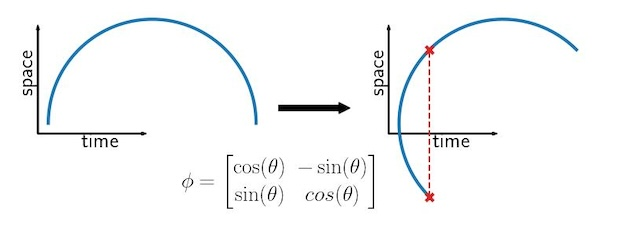
\includegraphics[width=0.7\linewidth]{"./pictures/diffeo.jpeg"}
  
  \caption{A time series' graph $\msg=\{(t,s(t)): \eqsp t\in\msi\} $ can lose its structure after applying a general diffeomorphism $\phi.\msg$: a time value can be related to two values on the space axis.}
  \label{fig:diffeo}
  
\end{figure}

\begin{figure*}[t]
  \centering
  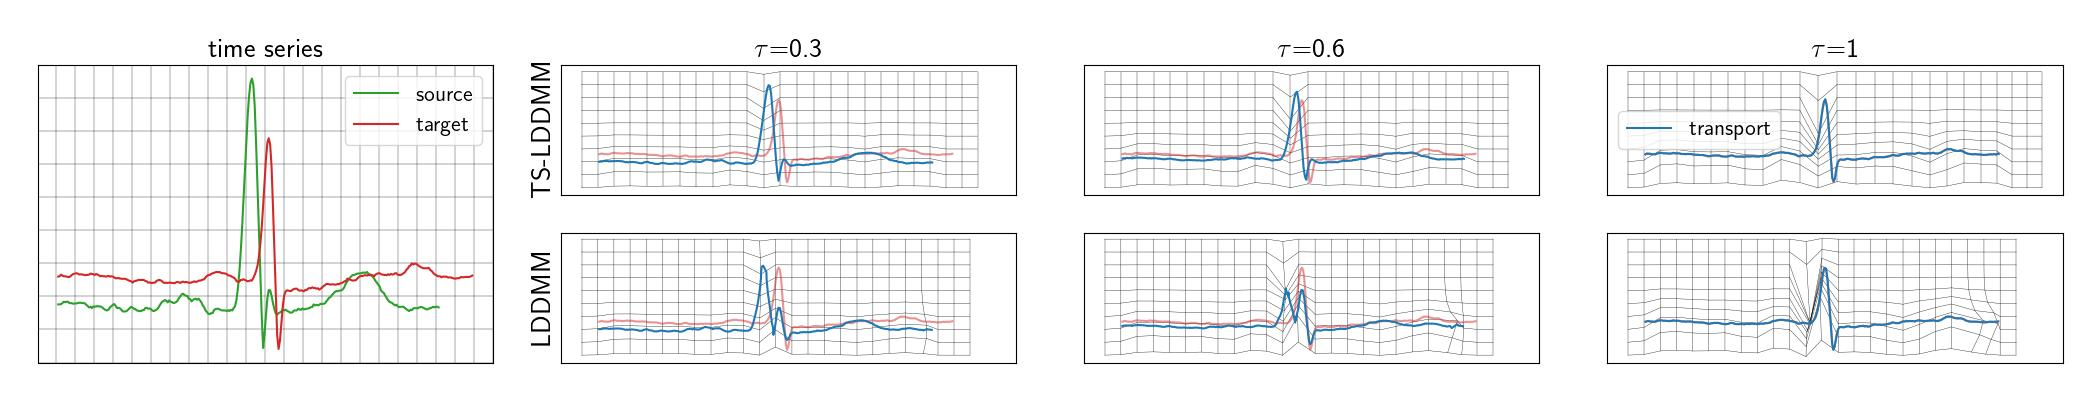
\includegraphics[width=\linewidth]{"./pictures/transport.jpeg"}
  
  \caption{LDDMM and TS-LDDMM are applied to ECG data.
  We observe that LDDMM, using a general Gaussian kernel, does not learn the time translation of the first spike but changes the space values, i.e., one spike disappears before emerging at a translated position. At the same time, TS-LDDMM handles the time change in the shape.
  This difference of \textit{deformations} implies differences in features \textit{representations}.   }
  \label{fig:transport}
  
\end{figure*}

\section{Related Works}
Shape analysis focus on the statistical analysis of various mathematical objects invariant under rotations, dilations, or time parameterization.
 The main idea is to represent these different objects in a complete Riemannian manifold $(\mathcal{M},\mathbf{g})$ with a metric $\mathbf{g}$ adapted to the geometry of the problem \cite{miller2006geodesic}.
 Then, any set of points in $\mathcal{M}$ can be represented as points in the tangent space of their Frechet mean $\mathbf{m}_0$ \cite{pal2017riemannian,le2001locating} by considering their logarithms.
 The goal is then to find a well suited Riemannian struvture according to the studied object.

 A time series graph can be seen as a curve and LDDMM structure is relevant to tackle curves as presented in \cite{glaunes2008large}. %, LDDMM structure is relevant to tackle curves and
  However, time series graph has more structure than curves as depicted in \Cref{fig:diffeo} due to the temporal evolution. 
  \cite{qiu2009time} tracks anatomical shape changes in serial images using LDDMM, but distinguish from us by including the temporal evolution at a higher level: the goal is to perform longitudinal data modeling.

  Leaving the LDDMM representation, \cite{srivastava2010shape,heo2024logistic} address the representation of curves having unitary velocity by using the Square-Root Velocity (SRV) representation.
 However, the SRV representation applies after a reparametrization in time, such that the original time evolution of the time series is not represented in the final features.
  Again, the time series graph structure is not respected.
   Very recently in a functionnal data analysis framework, a paper \cite{wu2024shape} (Shape-FPCA) improved by giving a representation for the original time evolution.
    Nevertheless, this methods applies only on time series of \textit{same size} and is made for \textit{continuous objects}, making the estimation more sensitive to noise.
  %However, the case of time series has not been adequately addressed, considering the special attention the time axis requires.
  %For instance, the SRV representation applies after a reparametrization in time, such that the original time evolution of the time series is not represented in the final features.
% Depending on the tasks, e.g classification \cite{ismail2019deep}, anomaly detection \cite{blazquez2021review}, forecasting \cite{torres2021deep} or clustering , a meaningful vector representation of time series can be derived.
%  Initially, in this research, handcrafted features were computed from time series, such as the mean, wavelets \cite{percival2000wavelet}, or Fourier coefficients \cite{bloomfield2004fourier}, depending on expert knowledge.
%   However, this approach is time-consuming and potentially biased by priors.
%   Observing the success of neural networks, features are automatically extracted by choosing an objective to optimize and a neural architecture tailored to the problem.
%    Taking a set of time series as input, features can be identified by solving specific supervised tasks—classification \cite{ismail2019deep}, anomaly detection \cite{blazquez2021review}, forecasting \cite{torres2021deep}— or in an unsupervised manner by deriving labels from the inputs \cite{meng2023unsupervised}.
%    \thi{Rajouter une image, et une phrase par rapport au temps}
%    Although the deep learning approach is particularly effective for supervised tasks, annotated datasets are rare, making unsupervised methods more practical.
%    These methods have proven effective in identifying different patterns in the data and providing a vector representation that segregates well into clusters \cite{meng2023unsupervised}.
%     However, they may lack precision on small and homogeneous datasets with only one typical shape, often arising from clinical experiments addressing a specific phenomenon (refer to figures).
%      While current unsupervised methods separate representations into clusters, our focus is on the inter-individual variability within one cluster.
%       Typically, we aim to perform Principal Components Analysis (PCA) \cite{bro2014principal} on individual patterns with similar shapes. The representation is dependant on the input dataset.
[Ajouter littérature de URL demander à Sisi ?]
 %\citet{srivastava2010shape,heo2024logistic} address the representation of curves $C:\msi \to \Rset^d$, $\msi\subset \Rset$, having unitary velocity by using the Square-Root Velocity (SRV) representation.
 %However, the case of time series has not been adequately addressed, considering the special attention the time axis requires.
 %For instance, the SRV representation applies after a reparametrization in time, such that the original time evolution of the time series is not represented in the final features.
 %In this regard, this work is not an application of LDDMM to 1D curves \cite{glaunes2008large}.
 %Compared to Normalizing Flows \cite{rezende2015variational,kobyzev2020normalizing} or Continuous Normalizing Flows \cite{chen2018neural,grathwohl2019scalable,salman2018deep} for diffeomorphisms learning, the number of hyperparameters to tune is minimal, and the related optimization problem is well-posed.
\section{Notations}
We denote by integer ranges by $[k:l]=\{k,\ldots,l\}\subset \mathcal{P}(\Zset)$ and $ [l]=[1:l]$ with $k,l\in \Nset$,
by $\rmC^m(\msi,\mse)$ the set of $m$-times continously differentiable function defined on an open set $\msu$ to a normed vector space $\mse$,
 by $||u||_\infty=\inf_{x\in \msu} |u(x)| $ for any bounded function $u:\msu \to \mse$,
and by $\Nset_{>0}$ is the set of positive integers. 
%We are in a sub class of curve quotiented by temporal reparametrisation since a time series' graph can be understood as the equivalent class of t ->(t,s(t))

%Reproducing Kernel Hilbert Space (RKHS)
\section{Background on LDDMM}
\label{section:LDDMM}

In this part, there is no novelty, we simply expose how to
 learn the diffeomorphisms $(\phi_j)_{j\in[N]}$ using LDDMM, initially introduced in \cite{beg2005computing}.
  In a nutshell, for any $j\in [N]$, $\phi_j$ corresponds to a differential flow related to a learnable velocity field belonging to a well-chosen Reproducing Kernel Hilbert Space (RKHS).

  In the next section, the time series are going to be represented by diffeomorphism parameters $(\alpha_j)_{j\in[N]}$.
  That's why LDDMM is chosen since it offers a parametrization for diffemorphisms which is sparse and interpretable, two features particularly relevant in the biomedical context.
 

The basic problem that we consider in this section is the following. Given a set of targets $\mathbf{y}=(y_i)_{i\in[T_2]}$ in $\Rset^{d'}$\footnote{Note that we denote by $d'\in\nset$ the ambient space}, a set of starting points $\mathbf{x}=(x_{i})_{i\in[T_1]}$ in $\Rset^{d'}$, we aim to find a diffeomorphism $\phi$ such that the finite set of points $\mathbf{y}$ is similar in a certain sense to the set of finite sets of transformed points $\phi \cdot \mathbf{x} =(\phi(x_i))_{i\in[T_1]} $.
 The function $\phi$ is occasionally referred to as a \textit{deformation}. In general, these sets $\mathbf{x},\mathbf{y}$ are meshes of continous objects, e.g surfaces, curves, images and so on.

 
% LDDMM is designed to analyzed an existing dataset, while NF and CNF are made to generalize a dataset for data augmentation.
\paragraph{Representing diffeomorpshims as deformations.}
Such \textit{deformations} $\phi$ are constructed via differential flow equations, for any $x_0\in \Rset^{d'} $ and $\tau\in[0,1]$:
\begin{equation}
  \label{eq:LDDMM_dynamic}
    \frac{\dd X(\tau)}{\dd \tau}= v_\tau(X(\tau)), \quad X(0)=x_0\eqsp ,
    \phi^v_\tau(x_0)=X(\tau), \quad \phi^v=\phi^v_1  \eqsp ,
\end{equation}
where the velocity field is $v:\tau\in [0,1]\mapsto v_\tau\in \msv $
and $\msv$ is a Hilbert space of continuously differentiable function
on $\Rset^{d'}$.  If
$||\dd u ||_{\infty}+|| u ||_{\infty}\leq ||u ||_\msv $ for any
$u\in \msv$ and
$v\in \rml^2([0,1],\msv)=\{v\in \rmC^0([0,1],\msv): \int_0^1 ||
v_\tau||^2_\msv \dd \tau<\infty \} $, by \citep[Theorem 5]{glaunes2005transport}
$\phi^v$ exists and belongs to $\mcd(\Rset^{d'})$, where we denote by $\mcd(\mso) $ the set of diffeomorpshim defined on an open set $\mso$ to $\mso$.
 Therefore, for any choice of $v$, $\phi^v$ defines a valid deformation. 
This offers a general recipe to construct diffeomorphism given a functional space $\msv$.

With this in mind, the velocity field $v$ fitting the data can be
estimated by minimizing 
$v \in \rml^2([0,1],\msv) \mapsto \mathscr{L}(\phi^{v}.\mathbf{x},\mathbf{y})$, where $\mathscr{L}$ is an appropriate loss function.
 However, two computational challenges arise.
  First, this optimization problem is ill-posed, and a penalty term is needed to obtain a unique solution.
   In addition, we have to find a parametric family $\msv_{\Theta} \subset \rml^2([0,1],\msv)$, parameterized by $\Theta$, which allows us to solve this minimization problem efficiently. 

%\paragraph*{Regularizing the problem to derive uniqueness.}
It has been proposed in \cite{miller2006geodesic} to interpret $\msv$ as a tangent space relative to the group of diffeomorphisms $\msh=\{ \phi^v:\eqsp v\in \rml^2([0,1],\msv)\}$.
Following this geometric point of view, geodesics can be constructed on $\msh$ by using the following squared norm 
 \begin{equation}
  \label{eq:geodesics_original}
    \mathscr{R}^2: g\in \msh\mapsto \inf_{ v\in \rml^2([0,1],\msv):\eqsp g=\phi^v} \int_0^1 || v_\tau||_\msv\dd \tau
 \end{equation}
By deriving differential constraints related to the minimum of \eqref{eq:geodesics_original} and using Cauchy lipshcitz conditions, geodesics can be defined only by giving the starting point and the initial velocity $v_0\in \msv$ \cite{miller2006geodesic}, as straight lines in Euclidean space.
Denoting by $w(v_0)$ the geodesic starting from the identity with inital velocity $v_0$, the exponential map is defined as $\varphi^{\{v_0\}}\triangleq \phi^v$ and the previous matching problem becomes a \textit{geodesic shooting problem}:
 \begin{equation}
  \label{eq:geodesics_shooting}
  \inf_{v_0 \in \msv} \mathscr{L}(\varphi^{\{v_0\}}.\mathbf{x},\mathbf{y}).
 \end{equation}
 Using $\varphi^{\{v_0\}}$ instead of $\phi^v$ for any $v\in \rml^2([0,1],\msv)$ regularizes the problem and induces a sparse representation for the learning diffeomorphisms.
 Moreover, by setting $\msv$ as an RKHS, the geodesic shooting problem has a unique solution and becomes tractable, as described in the next section.




% More precisely, on the group of diffeomorphisms $\msh=\{ \phi^v:\eqsp v\in \rml^2([0,1],\msv)\}$,
%  the following squared norm can be defined
%  \begin{equation}
%   \label{eq:geodesics_original}
%     \mathscr{R}^2: g\in \msh\mapsto \inf_{ v\in \rml^2([0,1],\msv):\eqsp g=\phi^v} \int_0^1 || v_\tau||_\msv^2\dd \tau
%  \end{equation}
%      as the minimal "energy" needed to perform the deformation $g$.
% By \citep[Theorem 6]{glaunes2005transport}, there exists $v^*\in \rml^2([0,1],\msv)$ such that the previous infimum is a minimum in $v^*$ such that $(\phi^{v^*}_\tau)_{\tau\in[0,1]}$ can be understood as the geodesic between the identity function and $g$.
% However, given a diffeomorphism $g$, computing $\mathscr{R}(g)$ is intractable in most cases. 
% To circumvent this issue, another characterization of geodesics can be considered.
%  As in Riemannian geometry, 
%  instead of defining geodesics from their starting and end points, it is possible to define them from their starting point (here, the identity function) and an initial velocity $v_0\in\msv$.
%  \sam{To CHANGE}
%  %In other words, an Exponential map on deformations is wanted:
% given $v_0\in\msv$, it has been suggested to generate diffeomorphisms as $\varphi^{\{v_0\}}=\phi^v$ with
% %  \begin{equation}
% %   \label{eq:geodesics_shooting}
% %   v=\underset{w\in \rml^2([0,1],\msv):\eqsp w_0=v_0}{\argmin} \int_0^1 || w_\tau||_\msv^2\dd \tau\eqsp ,
% %  \end{equation}
% % since with this definition it holds $\mathscr{R}^2(\phi^v)= \int_0^1 || v_\tau||_\msv^2\dd \tau $.
%  By setting $\msv$ as an RKHS, the geodesic shooting problem \eqref{eq:geodesics_shooting} has a unique solution and becomes tractable, as described in the next section.
% Moreover, we have $\mathscr{R}(\varphi^{\{v_0\}})=||v_0||_\msv$ such that we can work with $v_0\in \msv $ instead of $v\in \rml^2([0,1],\msv)$.
%  Therefore, compared to CNF, only $v_0$ is parametrized by using the geodesic structure and not each $v_\tau$ for any $\tau\in[0,1]$.
%  Moreover, we have $\mathscr{R}(\phi^{\{v_0\}})=||v_0||_\msv$ such that we can work with $v_0\in \msv $ instead of $v\in L^2([0,1],\msv)$.
%  %Therefore, compared to CNF, only $v_0$ is parametrized by using the geodesic structure and not each $v_\tau$ for any $\tau\in[0,1]$.
%  This is presented with more details in the next paragraph.





\paragraph{Discrete parametrization of diffeomorpshim.}
%\alain{adapt this without mentioning applicaiton to time seriess}
%\sam{Est ce qu'on devrait pas introduire la dicretization du graphe ici et dire que l'on peut utiliser le théoreme de représentation}
In this part, $\msv$ is chosen as an RKHS \cite{berlinet2011reproducing} generated by a smooth kernel $K$ (e.g., Gaussian). % $K(x,y)\triangleq \exp(-|x-y|^2/\sigma^2)\operatorname{Id}_{d'}$ for any $(x,y)\in(\Rset^{d'})^2$, where $\sigma^2>0$ is the kernel width and $\operatorname{Id}_{d'}$ is the identity matrix.
We follow \cite{durrleman2013sparse} and define a 
 discrete parameterization of the velocity fields to perform geodesics shooting \eqref{eq:geodesics_shooting}.  
  The initial velocity field $v_0$ is chosen as a finite linear combination of the RKHS basis vector fields, 
$\mathbf{n}_0$ control points $\msx_0=(x_{k,0})_{k\in[\mathbf{n}_0]}\in (\Rset^{d'})^{\mathbf{n}_0}$ and momentum vectors $\alpha_0=(\alpha_{k,0})_{k\in[\mathbf{n}_0]}\in (\Rset^{d'})^{\mathbf{n}_0} $ are defined such that for any $x\in \Rset^{d'}$, 
  \begin{equation}
    \label{eq:def_v0}
    v_0\left(\alpha_0,\msx_0\right)(x)=\sum_{k=1}^{\mathbf{n}_0} K(x,x_{k,0})\alpha_{k,0} \eqsp .
  \end{equation}
   In our applications, the control points $(x_{k,0})_{k\in[\mathbf{n}_0]}$ can be understood as the discretized graph $(t_k,\mathbf{s}_0(t_k))_{k\in[\mathbf{n}_0]}$ of a starting time series $\mathbf{s}_0$. 
  With this parametrization of $v_0$, \citet{miller2006geodesic} show that the velocity field $v$ of the solution of \eqref{eq:geodesics_shooting} keeps the same
  structure along time, such that for any $x\in\Rset^{d'}$ and $\tau\in[0,1]$, 
  \begin{equation}
    \label{eq:specific_form}
    v_\tau(x)=\sum_{k=1}^{\mathbf{n}_0} K(x,x_k(\tau))\alpha_{k}(\tau) \eqsp ,
  \end{equation}
  \begin{equation} 
    \label{eq:integration}
      \left\{
        \begin{aligned}
        & \frac{\dd x_k(\tau)}{\dd \tau}=v_\tau(x_k(\tau)) \eqsp, \quad
        \frac{\dd \alpha_k(\tau)}{\dd \tau}=-\sum_{k=1}^{\mathbf{n}_0} \dd_{x_k(\tau)} K(x_k(\tau),x_l(\tau))\alpha_{l}(\tau)^\top \alpha_{k}(\tau) \eqsp  \\
        & \alpha_k(0)=\alpha_{k,0},\quad x_k(0)=x_{k,0} \eqsp , k\in[\mathbf{n}_0] 
        \end{aligned}
        \right .
  \end{equation}
  These equations are derived from the hamiltonian $H:(\alpha_k,x_k)_{k\in [\mathbf{n}_0]}\mapsto \sum_{k,l=1}^{\mathbf{n}_0} \alpha_{k}^\top K(x_k,x_l)\alpha_{l}  $, such that
  the velocity norm is preserved $||v_\tau||_{\msv}=||v_0||_\msv $ for any $\tau\in [0,1]$.
   By \eqref{eq:integration}, the velocity field related to a geodesic $v^*$ is fully parametrized by its initial control points and momentum $(x_{k,0},\alpha_{k,0})_{k\in[\mathbf{n}_0]}$.
   Thus, given a set of targets $\mathbf{y}=(y_i)_{i\in[T_2]}$ in $\Rset^{d'}$, a set of starting points $\mathbf{x}=(x_{i,0})_{i\in[T_1]}$ in $\Rset^{d'}$, a RKHS's kernel $K:\Rset^{d'}\times \Rset^{d'}\to \Rset^{d'\times d'}$, a distance on sets $\mathscr{L}$, 
 a numerical integration scheme of ODE and a penalty factor $\lambda>0$, the basic geodesic shooting step minimizes the following function using a gradient descent method:
   \begin{equation}
    \label{eq:relaxation}
    \mathcal{F}_{\mathbf{x},\mathbf{y}}: (\alpha_k)_{k\in [T_1]}\mapsto \mathscr{L}\left(\varphi^{\{v_0\}}.\mathbf{x},\mathbf{y}\right)+\lambda||v_0||_\msv^2 \eqsp,  
   \end{equation}
   where $v_0$ is defined by \eqref{eq:def_v0} and $\varphi^{\{v_0\}}.\mathbf{x}$ is the result of the numerical integration of \eqref{eq:integration} using control points $\mathbf{x}$ and initial momentums $(\alpha_k)_{k\in[T_1]} $. 



   %Before to specify the choice of the RKHS kernel $K$ and the loss on sets $\mathscr{L}$ in \Cref{section:time_series_specificity}, we first discuss the connection of LDDMM with normalizing flows. % to highlight the interest of the LDDMM approach.


  
   
%Conversely to NF or CNF, by \eqref{eq:integration}, different momentums parameters raise different final deformations $\phi^{\{v_0\}}$, this injectivity properties offers interpretability of the representation and gives sens to PCA or LDA post-processing as exposed in \Cref{section:experiments}.
  
   %If a diffeomorpshim $\Phi$ is given and we want to represent it as a deformation $\phi^v$ with $v$ of minimal ernergy, then
  %$(\alpha_{k,0})_k$ is the only parameters to learn since $(x_{k,0})_k$ is fixed.
  


%   \begin{algorithm}[tb]
%     \caption{Geodesic shooting with LDDMM}
%     \label{alg:example}
%  \begin{algorithmic}
%     \STATE {\bfseries Input:} a RKHS's kernel $K$, a loss on sets $L$, $\mathbf{x}=(x_{i,0})_{i\in[T_1]}$, $\mathbf{y}=(y_i)_{i\in[T_2]}$ two sets of $\Rset^{d'}$, initial momentums 
%     $(\alpha_{k,0})_{k\in [T_1]} \in (\Rset^{d'})^{T_1}$ and a number of gradient iterations $n_{\text{iter}}$.

%     \STATE $f: (\alpha_k)_k\mapsto L\left(\phi^{\{v_0\}}.\mathbf{x},\mathbf{y}\right)+\lambda||v_0||_\msv^2  $ with $v_0$ and $\phi^{\{v_0\}}$
%      respectively defined by \eqref{eq:def_v0} and \eqref{eq:integration} using control points $\mathbf{x}$ and initial momentums $(\alpha_k)_k $. 
%      \sam{Peut être à définir dans un autre algo ?}
%     \STATE $\alpha_{k,0}^*\gets \alpha_{k,0}, \eqsp k\in[T_1]$
%     \FOR{$i=1$ {\bfseries to} $n_{\text{iter}}$}
%     \STATE $\alpha_{k,0}^*\gets \text{AdamStep}(f,\alpha_{k,0}^*$) , where $\text{AdamStep}$ is given in appendix (mettre ref)
%     \ENDFOR
%     \STATE {\bfseries Return:} $(\alpha_{k,0}^*)_{k\in [T_1]}$
    
%  \end{algorithmic}
%  \end{algorithm}
\paragraph{Relation to Continuous Normalizing Flows.}

One particular popular choice to address the problem of learning a diffeomorphism or a velocity field is Normalizing Flows \cite{rezende2015variational,kobyzev2020normalizing} (NF) or their continuous counterpart \cite{chen2018neural,grathwohl2019scalable,salman2018deep} (CNF).
However, we do not rely on this class of learning algorithms for several reasons. Indeed, existing and simple normalizing flows are not suitable for the type of data that we are interested in this paper \cite{feng2023multi,deng2020modeling}. 
  In addition,  they are primarily designed to have tractable Jacobian functions, while we do not require such property in our applications. 
Finally, the use of a differential flow solution of an ODE
\eqref{eq:LDDMM_dynamic} trick is also at the basis of CNF, which
then consists of learning a velocity field to address in fitting the data through a loss aiming to address the problem
at hand. Nevertheless, the main difference between CNF and LDDMM lies in the
parametrization of the velocity field. LDDMM uses kernels to
derive closed form formula and enhance interpretability while
NF and CNF take advantage of deep neural networks to scale with
large dataset in high dimensions.
\section{Methodology}
%\paragraph{Assumptions}
%Denoting by $C^0(\msi,\msj) $ the space of continous functions between two sets $\msi,\msj$,

We consider in this paper observations which consist in a population of $N$ multivariate time series, for any $j\in[N]$, $s^j \in \rmC^1(\msi_j,\Rset^{d})$. 
However, we can only access a $n_j$-samples $\tsig^j=(\tsig_i^j=s^j(t^j_i))_{i\in[n_j]}$ collected at timestamps $(t^j_i)_{i\in[n_j]}$ for any $j \in [N]$.
 Note that \textbf{the number of samples $n_j$ is not necessary the same accross individuals} and the timestamps can be \textbf{irregularly sampled}.
%To ease the presentation of our methodology, we suppose that we have access to the continuous time series $(s^j)_{j\in[N]}$, while in practice, we can only access a $n_j$-samples $\tsig^j=(\tsig_i^j=s^j(t^j_i))_{i\in[n_j]}$ collected at timestamps $(t^j_i)_{i\in[n_j]}$ for any $j \in [N]$.
 %However, this difference does not change the overall rationale of our method and its implementation up to minor changes, which we summarize in \eqref{eq:general_optimization_problem}.
 We assume the time series population is globally homogeneous regarding their "shapes" even if inter-individual variability exists.
 Intuitively speaking, the "shape" of a time series $s:\msi\to \Rset^d$ is encoded in its graphs $\msg(s)$ defined as the set $\{(t,s(t)):\eqsp t\in\msi \} $ and not only in its values $s(\msi)=\{s(t):\eqsp t\in\msi \} $ since the time axis is crucial. % on the shape as illustrated in Figure\alain{ (mettre ref)}.
 As a motivating use-case, $s^j$ can be the time series of a heartbeat extracted from an individual's electrocardiogram (ECG), see \Cref{fig:transport}.
 The homogeneity in a resulting dataset comes from the fact that humans have similar shapes of heartbeat \cite{ye2012heartbeat,madona2021pqrst}.
 % the shape is also referred as morphology of the time series. 
  %  [More specifically, the heterogeneity in such dataset is often due to local or glocal dilatation of the time series regarding time, the heartbeat is quicker or slower depending on the individual.
  %  In maths, denoting by $\mcd(\msi,\msj) $ the set of diffeomorpshim defined on the sets $\msi$ to $\msj$,
  %   there exist a common pattern $\mathbf{s}_0: \msi \to \Rset^d$ and individual time reparametrisations $ \psi_j\in\mcd(\msi,\msi_j) $ such that,
  %   for any $j\in[N]$, $s^j=\mathbf{s}_0\circ \psi_j^{-1} $.]
%  \paragraph{Goals}%\sam{potentiellement changer l'ordre de time and space}
\paragraph*{The deformation problem.}
In this paper, we aim to study the inter-individual variability in the dataset by finding a relevant representation of each time series.
Inspired from the framework of shape analysis \cite{vaillant2004statistics}, addressing similar problems in morphology,
 we suggest to represent each time series' graph $\msg(s^j)$ as the transformation of a reference graph $\msg(\mathbf{s}_0)$, related to a time series $\mathbf{s}_0:\msi \to\Rset^d$, by a diffeomorphism $\phi_j$ on $\Rset^{d+1}$, for any $j\in[N]$,
\begin{equation}
 \label{eq:transformation}
 \phi_j.\msg(\mathbf{s}_0)=\{\phi_j\left(t,\mathbf{s}_0(t)\right), \eqsp t\in \msi \} \eqsp.
\end{equation}
$\bfs_0$ will be understood as the typical representative shape common to the collection of time series $(s^j)_{j\in[N]}$.
As $\bfs_0$ is supposed to be fixed, then the representation of the time series $(s^j)_{j\in[N]}$ boils down to the one of the transformation $(\phi_j)_{j\in[N]}$.
We aim to learn $\msg(\bfs_0)$ and $(\phi_j)_{j\in[N]} $. 

%First, we introduce the Large Deformation Diffeomorphic Metric Mapping (LDDMM) framework.
% Then, we explain how to learn a discretization of the graph $\msg(\bfs_0)$ and the diffeomorphisms $(\phi_j)_{j\in[N]} $ by using LDDMM and a gradient descent minimization.
  %Finally, we tackle the specificity of graph time series by deriving a representation theorem on diffeomorphisms, which enables us to select the kernel needed in LDDMM, and thus, we propose TS-LDDMM. 
 
 
     %\sam{Parler de l'unicté?}
     \paragraph{Optimization related to \eqref{eq:transformation}.}
     Defining the \textit{discretized graphs} of the time series $(s^j)_{j\in[N]}$ and a discretization of the reference graph $\msg(\mathbf{s}_0)$  as, for any $j\in[N]$,
     \begin{equation}
      \label{eq:descretized_graph}
      \mathbf{y}_j=\msg(\tsig^j)=(t_i^j,\tsig^j_i)_{ i\in[n_j]}\in (\Rset^{d+1})^{n_j},\quad \tilde{\msg}_0=(t_i^0,\tsig^0_i)_{i\in[\mathbf{n}_0]}\in (\Rset^{d+1})^{\mathbf{n}_0} \eqsp ,
     \end{equation}
       with $\mathbf{n}_0=\operatorname{median}((n_j)_{j\in[N]})$, the representation problem given in \eqref{eq:transformation} boils down solving:
      \begin{equation}
        \label{eq:general_optimization_problem}
        \argmin_{\tilde{\msg}_0,(\alpha_k^j)_{k\in [\mathbf{n}_0]}^{j\in[N]}} \sum_{j=1}^N \mathcal{F}_{\tilde{\msg}_0,\mathbf{y}_j}\left((\alpha_k^j)_{k\in [\mathbf{n}_0]}\right)\eqsp ,
      \end{equation}
      which is carried out by a gradient descent on the control points $\tilde{\msg}_0$ and the momentums $\mathbf{\alpha}_j=(\alpha_k^j)_{k\in [\mathbf{n}_0]}$ for any $j\in[N]$, initialized by a dataset's time series graph of size $\mathbf{n}_0$ and by $0_{(d+1)\mathbf{n}_0}$ respectively.
      The optimization hyperparameter details are given in \Cref{appendix:optimizers_details}.
     The result of the minimization $\tilde{\msg}_0$ is then considered as the $\mathbf{n}_0$-samples of a common time series $\mathbf{s}_0$ and the momentums $\mathbf{\alpha}_j$ encoding $\phi_j$ yields a feature vector in $\Rset^{d \mathbf{n}_0} $ of $s^j$ for any $j\in[N]$.
     %, which will be the representation of the time series when choosing the time series' graph sets as inputs, is dependent on the choice of kernel $K$ and the set distance $L$.
     Finally, the vectors $(\mathbf{\alpha}_j)_{j\in[N]}$ can be analyzed with any statistical or machine learning tools such as Principal Components Analysis (PCA), Latent Discriminant Analysis (LDA), longitudinal data analysis and so on.
%As $\bfs_0$ is supposed to be fixed, then the representation of the time series $(s_j)_{j\in[N]}$ boils down to the one of the transformation $(\phi_j)_{j\in[N]}$.
 %In \Cref{section:optimization} the choice of the common time series $\mathbf{s}_0$ will be optimized to have $\phi_j$ of minimal norm. %T is given in the following part.

%  To learn the diffeomorphisms $(\phi_j)_{j\in[N]}$, we propose to use in this paper Large Deformation Diffeomorphic Metric Mapping (LDDMM).
%   In a nutshell, for any $j\in [N]$, $\phi_j$ corresponds to a differential flow related to a learnable velocity field belonging to a well-chosen Reproducing Kernel Hilbert Space (RKHS).
% We now describe more precisely LDDMM and in a next step the procedure to learn $\mathbf{s}_0$.

% \sam{to improve ?}
% Compared to the litterature of Unsupervised Representation Learning (URL) \cite{meng2023unsupervised}, the homogeneity assumption can be quite restrictive, however this is quite common in Shape Analysis \cite{vaillant2004statistics} (SA).
%     While in URL the goal is to find features accounting for the clustering structure in the heterogene data and to transfer this representation for different ML tasks, in SA the goal is to analyze the inter-individual variability with precision to derive clinical conclusions.
%     The generalization of the method presented in this paper to heterogene dataset is possible, but relagated for future works.
  %These velocity fields are then learned by minimizing the norm of this RKHS.

%In all the following, we denote by $\mcd(\mso) $ the set of diffeomorpshim defined on an open set $\mso$ to $\mso$.
%\sam{Transformer , en : dans les ensembles}

   %\sam{Parler de l'unicté?}


   %Before to specify the choice of the RKHS kernel $K$ and the loss on sets $\mathscr{L}$ in \Cref{section:time_series_specificity}, we first discuss the connection of LDDMM with normalizing flows. % to highlight the interest of the LDDMM approach.


  
   
%Conversely to NF or CNF, by \eqref{eq:integration}, different momentums parameters raise different final deformations $\phi^{\{v_0\}}$, this injectivity properties offers interpretability of the representation and gives sens to PCA or LDA post-processing as exposed in \Cref{section:experiments}.
  
   %If a diffeomorpshim $\Phi$ is given and we want to represent it as a deformation $\phi^v$ with $v$ of minimal ernergy, then
  %$(\alpha_{k,0})_k$ is the only parameters to learn since $(x_{k,0})_k$ is fixed.
  


%   \begin{algorithm}[tb]
%     \caption{Geodesic shooting with LDDMM}
%     \label{alg:example}
%  \begin{algorithmic}
%     \STATE {\bfseries Input:} a RKHS's kernel $K$, a loss on sets $L$, $\mathbf{x}=(x_{i,0})_{i\in[T_1]}$, $\mathbf{y}=(y_i)_{i\in[T_2]}$ two sets of $\Rset^{d'}$, initial momentums 
%     $(\alpha_{k,0})_{k\in [T_1]} \in (\Rset^{d'})^{T_1}$ and a number of gradient iterations $n_{\text{iter}}$.

%     \STATE $f: (\alpha_k)_k\mapsto L\left(\phi^{\{v_0\}}.\mathbf{x},\mathbf{y}\right)+\lambda||v_0||_\msv^2  $ with $v_0$ and $\phi^{\{v_0\}}$
%      respectively defined by \eqref{eq:def_v0} and \eqref{eq:integration} using control points $\mathbf{x}$ and initial momentums $(\alpha_k)_k $. 
%      \sam{Peut être à définir dans un autre algo ?}
%     \STATE $\alpha_{k,0}^*\gets \alpha_{k,0}, \eqsp k\in[T_1]$
%     \FOR{$i=1$ {\bfseries to} $n_{\text{iter}}$}
%     \STATE $\alpha_{k,0}^*\gets \text{AdamStep}(f,\alpha_{k,0}^*$) , where $\text{AdamStep}$ is given in appendix (mettre ref)
%     \ENDFOR
%     \STATE {\bfseries Return:} $(\alpha_{k,0}^*)_{k\in [T_1]}$
    
%  \end{algorithmic}
%  \end{algorithm}

Nevertheless, \eqref{eq:general_optimization_problem} ask to define a kernel and a loss in order to perform geodesic shooting \ref{eq:relaxation}, which is the purpose of the next subsection.
   \subsection{Application of LDDMM to time series analysis: TS-LDDMM}
%\tcr{Mettre l'applicaiton clair pour les times series}

        \label{section:time_series_specificity}
        In this section, we present our theoretical contribution: we tailor the LDDMM framework to handle time series data.
          The reason is that applying a general diffeomorphism $\phi$ from $\Rset^{d+1}$ to a time series' graph $\msg(s)$ can result in a set $\phi.\msg(s)$ that does not correspond to the graph of any time series, as illustrated in the \Cref{fig:diffeo}.
           Thus, Time series graph have more structure than a simple 1D curve \cite{glaunes2008large} and deserve their special analysis which will prove fruitful as demonstrated in \ref{section:experiments}.% thus this case is not an application of \cite{glaunes2004diffeomorphic}

To address this challenge, we need to identify an RKHS kernel $K:\Rset^{d+1}\times \Rset^{d+1}\to \Rset^{(d+1)^2}$ that generates deformations preserving the structure of the time series graph. This goal motivates us to clarify, in \Cref{theorem:representation}, the specific representation of diffeomorphisms we require before presenting a class of kernels that produce deformations with this representation.

Similarly, selecting a loss function on sets $\mathscr{L}$ that considers the temporal evolution in a time series' graph is crucial for meaningful comparisons with time series data. Consequently, we introduce the oriented Varifold distance. 
      
       \paragraph{A representation separating space and time.}
       We prove that two time series graphs can always be linked by a time transformation composed of a space transformation. Moreover, a time series graph transformed by this kind of transformation is always a time series graph.
        We define $\Psi_\gamma\in \mcd(\Rset^{d+1}) : (t,x)\in\Rset^{d+1}\to (\gamma(t),x)$ for any $\gamma\in \mcd(\Rset)$ and $\Phi_f:  (t,x)\in\Rset^{d+1}\to (t,f(t,x)) $ for any $f\in \rmC^1(\Rset^{d+1},\Rset^d)$. 
        We have the following representation theorem.
        All proofs are given in \Cref{appendix:proofs}. 


  Denote by $\msg(s)\triangleq \{ (t,s(t)): \eqsp t\in \msi \} $ the graph of a time series $s: \msi \to \Rset^d$ and $ \phi.\msg(s)\triangleq\{ \phi(t,s(t)): \eqsp t\in \msi\} $ the action of  $\phi\in \mcd(\Rset^{d+1}) $ on $\msg(s)$.
    \begin{theorem}
        \label{theorem:representation}
    Let $s:  \msj \to \Rset^d  $ and $\mathbf{s}_0: \msi\to \Rset^d $ be two continuously differentiable time seriess with $\msi,\msj$ two intervals of $\Rset$.
     There exist $f\in \rmC^1(\Rset^{d+1},\Rset^d)$ and $\gamma\in  \mcd(\Rset) $ such that $\gamma(\msi)=\msj $ and $\Phi_f\in \mcd(\Rset^{d+1})$,
     \begin{equation}
        \msg(s)= \Pi_{\gamma,f}.\msg(\mathbf{s}_0),\eqsp \Pi_{\gamma,f}=\Psi_\gamma\circ\Phi_f.
     \end{equation}
     Moreover, for any $\bar{f}\in \rmC^1(\Rset^{d+1},\Rset^d)$ and $\bar{\gamma}\in  \mcd(\Rset) $, there exists a continously differentiable time series $\bar{s}$ such that 
     $\msg(\bar{s})= \Pi_{\bar{\gamma},\bar{f}}.\msg(\mathbf{s}_0)$
    \end{theorem}
    %\sam{preuve todo, classement des variétés à bord, donne un homeomorphisme sur la restriction}
    % \begin{proof}
    %   Let $s:  \msj \to \Rset^d  $ and $\mathbf{s}_0: \msi\to \Rset^d $ be two continuously differentiable time seriess with $\msi=(a,b),\msj=(\alpha,\beta)$ two intervals of $\Rset$.
    %   % $\msg(\mathbf{s}_0)$ and $\msg(s)$ are two smooth connected 1-dimensional manifold of $\Rset^{d+1}$, thus, by \cite[Appendix
    %   % Classfying 1-Manifolds]{milnor1965topology}, there exists $\Pi\in \mcd(\Rset^{d+1})$ such that $\msg(s)=\Pi.\msg(\mathbf{s}_0)$.
    %   %  Therefore, denoting by $\Pi_1: \Rset^{d+1}\mapsto \Rset$, we define $\gamma(t)\triangleq \Pi_1(t,\mathbf{s}_0(t))$ for any $t\in \msi$, then for any $t\in [b,+\infty)$,
    %   %   \begin{equation}
    %   %     \gamma(t)=\\Pi_1(b,\mathbf{s}_0(b))+(t-b)\frac{\dd\gamma}{\dd^- t}(b) \eqsp,
    %   %   \end{equation}
    %   %   and for any $t\in (-\infty,a]$,
    %   %   \begin{equation}
    %   %      \gamma(t)=\Pi_1(a,\mathbf{s}_0(a))+(t-a)\frac{\dd\gamma}{\dd^+ t}(a)\eqsp ,
    %   %   \end{equation}
    %   %    where $ \frac{\dd\gamma}{\dd^- t},\frac{\dd\gamma}{\dd^+ t}$ are respectively the left and right derivative.
        
    %   By setting $\gamma: t\in \Rset \mapsto (\beta-\alpha)(t-a)/(b-a)+\alpha\in \Rset $, we have $ \gamma(\msi)=\msj$ and $\gamma \in \mcd(\Rset) $.
    %    By defining $f:(t,x)\in\Rset^{d+1}\mapsto x-\mathbf{s}_0(t)+s\circ \gamma(t) $, the map $\Phi_f\in \mcd(\Rset^{d+1})$,
    %     indeed, its inverse is $\Phi_f^{-1}:(t,x)\in\Rset^{d+1}\mapsto (t,x+\mathbf{s}_0(t)-s(t)) $ and is continuously differentiable.
    %      Moreover, we have $\Pi_{\gamma,f}.\msg(\mathbf{s}_0)=\{(\gamma(t),s\circ \gamma(t)):\eqsp t\in\msi \}=\msg(s) $.

        

    %     Let $\bar{f}\in \rmC^0(\Rset^{d+1},\Rset^d)$, $\bar{\gamma}\in  \mcd(\Rset) $ and $\mathbf{s}_0\in \rmC^0(\msi,\Rset^d)$ with $\msi$ an interval of $\Rset$.
    %     We have :
    %     \begin{align}
    %       \Pi_{\gamma,f}.\msg(\mathbf{s}_0)&=\{(\gamma(t),f(t,\mathbf{s}_0(t))),\eqsp t\in \msi \} \\
    %       &\label{eq:proof1_last_eq}=\{(t,f\left(\gamma^{-1}(t),\mathbf{s}_0(\gamma^{-1}(t))\right),\eqsp t\in \gamma(\msi) \} \eqsp .
    %     \end{align}
    %     By defining $\bar{s}:t\in \gamma(\msi)\to f\left(\gamma^{-1}(t),\mathbf{s}_0(\gamma^{-1}(t))\right) $, we have $\bar{s}\in \rmC^0(\gamma(\msi), \Rset^d) $ by composition of continuous functions
    %     and $ \msg(\bar{s})= \Pi_{\gamma,f}.\msg(\mathbf{s}_0)$ by \eqref{eq:proof1_last_eq}, which concludes the proof.
    % \end{proof}
    \begin{remark}
      that for any $\gamma \in \mcd(\Rset) $ and $s\in \rmC^0(\msi,\Rset^d)$,
   \begin{equation}
    \{(\gamma(t),s(t)),\eqsp t\in \msi \}=\{(t,s\circ \gamma^{-1}(t)):\eqsp t\in\gamma(\msi) \}\eqsp .
   \end{equation}
   As a result, $\Psi_\gamma $ can be understood as a temporal reparametrization and $\Phi_f$ encodes the transformation about the space.
 \end{remark}


    \paragraph{Choice for the kernel associated with the RKHS $\msv$}
    \label{paragraph:kernel_V}
    As depicted on \Cref{fig:diffeo}-\ref{fig:transport}, we can not use any kernel $K$ to apply the previous methodology to learn deformations on time series' graphs.
    We describe and motivate our choice in this paragraph.
     Denote the one-dimensional Gaussian kernel by $K_\sigma^{(a)}(x,y)=\exp(-|x-y|^2/\sigma)$ for any $(x,y)\in (\Rset^a)^2$, $a\in \Nset$ and $\sigma>0$.
    To solve the geodesic shooting problem \eqref{eq:relaxation} on $\Rset^{d+1}$, we consider for $\msv$ the RKHS associated with the kernel defined for any $(t,x),(t',x')\in (\Rset^{d+1})^2$:
    \begin{align}
      \label{eq:kernel_TAS}
      &K_{\msg}((t,x),(t',x'))=\begin{pmatrix}
        c_0K_{\text{time}} & 0 \\
        0 & c_1 K_{\text{space}} 
        \end{pmatrix} \eqsp ,\\
       & K_{\text{space}}=K_{\sigma_{T,1}}^{(1)}(t,t')K_{\sigma_x}^{(d)}(x,x') \Idd\eqsp,K_{\text{time}}=K_{\sigma_{T,0}}^{(1)}(t,t') \eqsp,
    \end{align}
    parametrized by the widths $\sigma_{T,0},\sigma_{T,1},\sigma_x>0$ and the constants $c_0,c_1>0$.
This choice for $K_\msg$ is motivated by the representation \Cref{theorem:representation} and the following result. 
    \begin{lemma}
      \label{lemma:choice_of_kernel_V}
      If we denote by $\msv$ the RKHS associated with the kernel $K_{\msg}$, then for any vector field $v$ generated by \eqref{eq:integration} with $v_0$ satisfying \eqref{eq:def_v0},
       there exist $\gamma \in \msd(\Rset) $ and $f\in \rmC^1(\Rset^{d+1},\Rset^d)$ such that $\phi^v=\Psi_\gamma\circ\Phi_f $.
    \end{lemma}
    \sam{Parler des Cauchy kernel en appndice et du choix de la loss}
    % \begin{proof}
    %   Let $v$ be a vector field generated by \eqref{eq:integration} with $v_0$ satisfying \eqref{eq:def_v0}.
    %  We remark that the first coordinate of the velocity field $v_\tau$ denoted by $v_\tau^{\text{time}}$ only depends on the time variable $t$ for any $\tau\in[0,1]$.
    %  Thus, when computing the first coordinate of the deformation $\phi^v$, denoted by $\gamma$, we integrate \eqref{eq:LDDMM_dynamic} with $v_\tau$ replaced by $v_\tau^{\text{time}}$,
    %   thus $\gamma$ is independant of the variable $x$. Moreover, $\gamma\in \mcd(\Rset)$ since a Gaussian kernel induced an Hilbert space $\msv$ satisfying $|f|_V\leq |f|_\infty+ |\dd f|_\infty  $ for any $f\in \msv$ by \citep[Theorem 9]{glaunes2005transport}.
    %   For the same reason, we have $\phi^v\in \mcd(\Rset^{d+1})$, and thus its last coordinates denoted by $f$ belongs to $\rmC^1(\Rset^{d+1},\Rset^d)$, and by construction $\phi^v=\Psi_\gamma\circ\Phi_f $.
    % \end{proof
    \begin{remark}
      With this choice of kernel, the features associated to the time transformation can be extracted from the momentums $(\alpha_{k,0})_{k\in[\mathbf{n}_0]}\in (\Rset^{d+1})^{\mathbf{n}_0}$ in \eqref{eq:def_v0} by taking the coordinates related to time.
      However, the features related to the space transformation are not only in the space coordinates since the related kernel $K_{\text{space}}$ depends on time as well.
     \end{remark}
    In \Cref{appendix:kernel_TS_LDDMM}, we give guidelines for selecting the hyperparameters $(\sigma_{T,0},\sigma_{T,1},\sigma_x,c_0,c_1)$.
  
  
    

    %  and then we can perform a statistical analysis on the representations $(\psi_j,\phi^j)_{j\in[N]}$,
    % such as applying PCA decomposition \cite{vaillant2004statistics}, carring out longitudinal analysis \cite{guigui2022parallel} and so on (\sam{mettre ref}).
    % % Cette hypothèse intéressante car ça permet de gérer des signaux de taille variables, tout les signaux se repréentent comme ça 
    % % Espace homogène, injectivité de t ,s(t), permet de garder la structure temporel en compte
    % \sam{Can we show unicity by assuming that $\phi,\psi$ minimize a norm ?}
 % KEOPS tp pour lddmm




%and their empiric samples version $\tilde{G}_j=(\{(t_i,s^j_i), \eqsp i\in [n_i]\})_j $

%  We translate the notation from the continous to discrete by adding a tilde :
%   $\tilde{G}^j=\triangleq \{ (t_i,\tilde{s}_i^j),\eqsp i\in[n_i] \}$.

% \paragraph{A problem of minimization}
% In the next section, we will present that diffeomorpshim on space an time can be parametrized as $\phi^{v^S},\phi^{v^T}$
%  with parameters $(v^S,v^T) \in \Theta_S\times \Theta_T$. Then, pattern will be represented by the parameters $v^S,v^T$ solutions of the following minimization :
% \begin{align}
%   \label{eq:minimization}
%   &\argmin_{v^S \in \Theta_S,\eqsp v^T\in \Theta_T } \mathbf{D}(v^S,v^T)+\lambda \mathbf{N}(v^S,v^T)\eqsp , \\
%   & \mathbf{D}(v^S,v^T)=L(\phi^{v^S}.G^\msj(\mathbf{s_0}\circ (\psi^{v^T})^{-1}),G^\msj(s)) \eqsp , 
% \end{align} 
% where $L$ is a loss on graphs and $\mathbf{N}$ is a term of regularization.

 


% $s_i: t\in[0,T_0]\mapsto s(t)\in \Rset^d $ is only known through its samples $(S_i^j(t_i)=s_i)_{i\in[N]} $ at timestamps $(t_i)_{i\in[T]}$.

%\sam{améliorer transition}
\paragraph{Loss}

This section specifies the distance function $\scrl$ introduced in the loss function defined in \eqref{eq:relaxation}. 

In practice, we can only access discretized graphs of time series, $(t_i^j,\tsig^j_i)_{i\in[n_j]}$ for any $j\in[N]$, that are potentially of 
different sizes $n_j$ and sampled at different timestamps $(t_i^j)_{i\in[n_j]}$ for any $j\in[N]$.
 Usual metrics, such as the Euclidean distance, are not appealing as they 
make the underlying assumptions of equal size sets and the existence of a pairing between points.
 Distances between measures on 
sets (taking the empirical distribution), such as Maximum Mean Discaprency (MMD) \cite{dziugaite2015training,borgwardt2006integrating}, alleviate those issues; however, MMD only accounts for positional information 
and lacks information about the time evolution between sampled points.
 A classical data fidelity metric from shape analysis 
corresponding to the distance between \textit{oriented varifolds} associated with curves alleviates this last issue \cite{kaltenmark2017general}.  
Intuitively, an oriented varifold is a measure that accounts for positional and tangential information about the underlying 
curves at sample points. More details and information about \textit{oriented varifolds} can be found in \Cref{appendix:varifold}. 

More precisely, given two sets $\msg_0=(g_i^0)_{i\in[T_0]},\msg_1=(g_i^1)_{i\in[T_1]}\in (\Rset^{d+1})^{T_1}$ and a kernel\footnote{$\mathbb{S}^d=\{x\in\Rset^{d+1}:\eqsp |x|=1\}$} $k:(\Rset^{d+1} \times \mathbb{S}^d)^2\to \Rset$
verifying \citep[Proposition 2 \& 4]{kaltenmark2017general}, for any $\xi\in\{0,1\}$ and $i\in[T_\xi-1]$, denoting the center and length of the $i^{th}$ segment $[g_i^\xi,g_{i+1}^\xi]$ by
$c_i^\xi = (g_i^\xi + g_{i+1}^\xi)/2$, $l_i^\xi = \| g_{i+1}^\xi-g_{i}^\xi\|$, and 
$\overrightarrow{v_i}^\xi = (g_{i+1}^\xi-g_{i}^\xi)/l_i^\xi$, the varifold distance between $\msg_0$ and $\msg_1$  is defined as,
\begin{align}
  &d_{\msw^*}^2(\msg_0,\msg_1) = \sum_{i,j = 1}^{T_0-1}l^0_i k((c^0_i,\overrightarrow{v_i}^0),(c^0_j,\overrightarrow{v_j}^0))l^0_j
  - 2 \sum_{i=1}^{T_0-1}\sum_{j=1}^{T_1-1}l^0_i k((c^0_i,\overrightarrow{v_i}^0),(c^1_j,\overrightarrow{v_j}^1))l^1_j \\
  &+ \sum_{i,j = 1}^{T_1-1}l^1_i k((c^1_i,\overrightarrow{v_i}^1),(c^1_j,\overrightarrow{v_j}^1))l^1_j 
\end{align}

In practice, we set the kernel $k$ as the product of two anisotropic Gaussian kernels, $k_{\pos}$ and $k_{\dir}$, 
such that for any $(x,\overrightarrow{u}),(y,\overrightarrow{v}) \in (\Rset^{d+1} \times \mathbb{S}^d)^2$
\begin{equation}
    k((x,\overrightarrow{u}),(y,\overrightarrow{v})) = k_{\pos}(x,y)k_{\dir}(\overrightarrow{u},\overrightarrow{v}) \eqsp.
  \end{equation}
  The specific kernels $k_{\pos},k_{\dir}$ that we use in our experiments are given \Cref{appendix:kernel_implementation}.
   Note that the loss kernel $k$ has nothing to do with the velocity field kernel denoted by $K_\msg$ or $K$ specified in \Cref{paragraph:kernel_V}.
Finally, we define the data fidelity loss function, $\scrl$, as $ d_{\msw^*}^2$, which is differentiable with regards to its first variable.
For further readings on curves and surfaces representation as varifolds, readers can refer to \cite{kaltenmark2017general,charon2013varifold}. 


%\sam{TO improve by Thibaut
%\thi{parler du fait qu'on a pas pairing, grace au difféo on conserve la structure}
%To relax the geodesic problem \Cref{eq:geodesics_original}, the end point of the geodesics is compared to the target through a loss $\mathscr{L}$ as proposed in \eqref{eq:relaxation}.
%Since we are dealing with discrete time series $\tsig^j$ of different samples size $n_j$, we need a loss on set measures and not only on vectors.
% A natural choice would be the Maximum Mean Discrepency (MMD) \cite{dziugaite2015training,borgwardt2006integrating}, for any $X=(x_i)_{i\in[T_1]},Y=(y_i)_{i\in[T_2]}\subset Rset^{d'}$, given a kernel $k:\Rset^{d'}\times \Rset^{d'} \to \Rset$,
% \begin{align}
%  &\operatorname{MMD}^k(\mu_X,\mu_Y)=\frac{1}{T_1^2}\sum_{i,j=1}^{T_1} k(x_i,x_j)+\frac{1}{T_2^2}\sum_{i,j=1}^{T_2} k(y_i,y_j) \\
%  &-\frac{2}{T_1T_2}\sum_{i=1}^{T_1}\sum_{j=1}^{T_2} k(x_i,y_j) \eqsp , 
% \end{align}
% where $\mu_X=\sum_{i=1}^{T_1} \delta_{x_i}/T_1$, $\mu_Y=\sum_{j=1}^{T_2} \delta_{y_j}/T_2$.
%However, this distance is agnostic of the time evolutions in time series' graph $(t_i^j,\tsig^j_i)_{i\in[n_j]}$, there is no orientation of the set taken into account.
% That is why, we prefer to choose the Varifold distance $d_V(\cdot,\cdot)$ \cite{kaltenmark2017general} which was specifically designed for oriented curves.
%  The Varifold distance extends the MMD by adding tangent vectors to the input:
%   instead of considering a set $X=(x_i)_{i\in[T_1]}$, we extend the input as $\overrightarrow{X}=(x_i,v_i)_{i\in[T_1]}$ where $v_i$ is the tangent vector at $x_i$ such that
%    \begin{equation}
%      d_V(X,Y)=\operatorname{MMD}^{K_p}(\mu_{\overrightarrow{X}},\mu_{\overrightarrow{X}}) \eqsp ,
%    \end{equation}
%    where in practice the tangent vectors are taken as discrete derivative and $K_p$ is a kernel on $\Rset^{2d'}$ such that for any $(x,v),(y,w)\in (\Rset^{2d})^2$, 
%    we have, 
%    \begin{equation}
%      K_p((x,v),(y,w))=k(x,v)k_T(v,w) \eqsp ,
%    \end{equation}
%   where $k_T $ is a kernel on the tangent vector space.



\sam{Parler de méthode adaptatif ici}
  






%Wavelet-Based Multiscale Flow For Realistic Image Deformation in the Large Diffeomorphic Deformation Model Framework
% 3.1 +3.2 + specialité de la décomposition (t,f(t,x))
% \section{Specificity to time series}
% We are looking to time seriess 
% Each time series $s: t\in[0,T]\mapsto s(t) $ is only known through its samples $(s(t_i)=s_i)_{i\in[N]} $ at timestamps $(t_i)_{i\in[N]}$.
%is described by its graph $G(s)=\{(y,s(t)), \} $



% \section{optimzation
% % We are not doing Pre-ESPAce car l'on s'intéresse à la reparamétrisation en temps, au lieu de calculer la transfo en temps après avoir
% % push en espace, on le fait avant pour que tout soit défini depuis s_0, méthode itérative car ça marche mieux, moins de calcul de gradient
% %Natural smoothing with TTS
% \label{section:optimization}
%     \begin{center}
%         \begin{tikzpicture}
%             \node at (0,0) {$G_f^I$};
%             \draw [-stealth](0.3,0) -- (1.3,0);
%             \node at (1.6,0) {$G_f^J$};
%             \draw [-stealth](1.6,-0.3) -- (1.6,-1.3);
%             \node at (1.6,-1.6) {$G_g^J$};
%             \draw [-stealth](1.3,-1.6) -- (0.3,-1.6);
%             \node at (0,-1.6) {$G_g^I$};
%             \draw [-stealth](0,-1.3) -- (0,-0.3);
        
%             \node at (0.8,0.3) {$T$};
%             \node at (0.8,-1.9) {$T^{-1}$};
%             \node at (1.9,-0.8) {$S_J$};
%             \node at (-0.4,-0.8) {$S_I^{-1}$};
%         \end{tikzpicture}
%         \end{center}
    
%         where $S_I^{-1} = T^{-1} \circ S_J^{-1} \circ T$




\section{Experiments}
\label{section:experiments}
[L'intro est ce necessaire ?]


First, we show on synthetic data that the proposed representation is identifiable provided that the hyperparameters and the reference graph are wisely selected, i.e.,
 the parameter $v_0^*$ generating a deformation $\varphi^{\{v_0^*\}}$ of a time series graph $\msg$ can be estimated from the data $\msg,\varphi^{\{v_0^*\}}.\msg$ by solving the geodesic shooting problem \eqref{eq:relaxation}.
 Secondly, we illustrate the qualitative interest of TS-LDDMM in studying inter-individual variability on a clinical dataset.
  Thirdly, we demonstrate the quantitative performance of our representation by performing classification on shape-based datasets.
  The method is implemented on Python using the library JAX\footnote{https://github.com/google/jax}. The code was compiled on a server with NVIDIA RTX A2000 12GB GPU, Intel(R) Xeon(R) Gold 5220R CPU @ 2.20GHz, and 250 GB of RAM. The code will be available on Github.
\subsection{Synthetic experiments}
\begin{figure}[t]
    \centering
    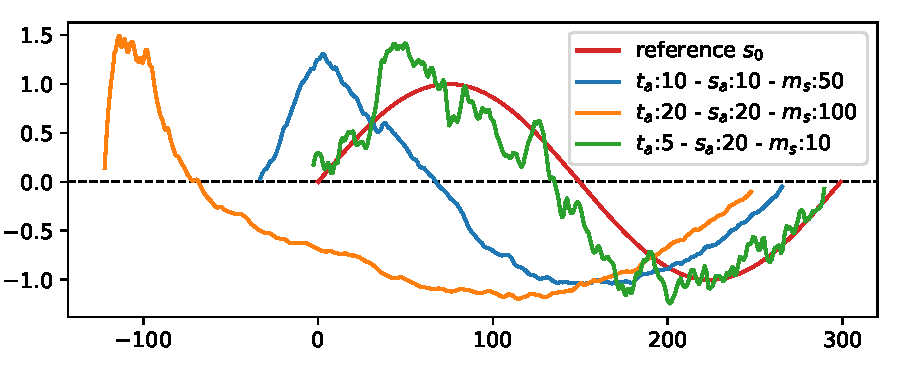
\includegraphics[width=0.5\linewidth]{pictures/samples.pdf}
    \vspace{-2.5em}
    \caption{Plots of $\varphi^{\{v_0(\mathbf{\alpha}^*,\msx)\}}.\msx$ for different values of $\mathbf{\alpha}^*$ according to its sampling parameter $t_a,s_a,m_s $, taking $\msx=\msg(s_0)$ with $s_0:k\in [300]\to \sin(2\pi k/300) $.}
    \label{fig:exemple_synthetic}
    \vspace{-1em}
\end{figure}

\begin{table}
    \caption{Values of $\scrl(\varphi^{\{v_0(\mathbf{\alpha}^*,\msx)\}}.\msx,\varphi^{\{\hat{v}_0\}}.\msx)$ as $\mathbf{\alpha}^*$ is sampled according to Gen(10,10,50) and $\hat{v}_0$ is estimated using $K_\msg$ with varying parameters $\sigma_{T,1},\sigma_x$.}
      \centering
         \begin{tabular}{lrrrrrrr}
         \toprule
         $\sigma_{T,0} \backslash \sigma_x$  & 1 & 10 & 50 & 100 & 200 & 300 \\
         \midrule
         0.1 & 2e+0 & 3e-4  & 1e-5&4e-6&7e-4&4e-3 \\
        1 & 4e-2 & 1e-4  & 1e-5&4e-6&7e-4 &4e-3  \\
         100 & 4e-2 & 2e-4  & 1e-5&4e-6&7e-4&4e-3  \\
         \bottomrule
         \end{tabular}
      \label{table:synthetic2}
      \vspace{-1em}
  \end{table}
 


% \begin{subfigure}{0.7\linewidth}
%   \centering
%   \resizebox{\columnwidth}{!}{%
%      \begin{tabular}{lrrrr}
%      \toprule
%      $\sigma_{T,0} \backslash \sigma_x$  & 0.1 & 1 & 100 \\
%      \midrule
%      1 & 2e+0 & 4e-2 & 4e-2 \\
%      10 & 3e-4 & 1e-4  & 2e-4 \\
%      50 & 1e-5 & 1e-5  & 1e-5 \\
%      100 & 4e-6 & 4e-6 & 4e-6 \\
%      200 & 7e-4 & 7e-4 & 7e-4 \\
%      300 & 4e-3 & 4e-3 & 4e-3 \\
%      \bottomrule
%      \end{tabular}
%      %
%      }
%  \caption{Values of $\scrl(y^*,\varphi^{\{\hat{v}_0\}}.\msx)$ where $y^*$ is sampled according to Gen(10,10,50) and $\hat{v}_0$ is estimated using $K_\msg$ with varying parameters $\sigma_{T,1},\sigma_x$.}
% \end{subfigure}
First, we show the model identifiability when the kernel $K_G$ is well specified: the estimated parameter is a good approximation of the generating parameter when the generation and the estimation procedure use the same hyperparameters for the RKHS kernel $K_\msg$.
All the hyperparameter values for generation and estimation are given in \Cref{appendix:numerics_synthetic}.
We fix the initial control points as $\msx=\left(x_k=(k,\sin(2\pi k/300))\right)_{k\in[300]} $.
Given $m_{s}\in \Nset_{>0}$ and $t_{a},s_{a}>0$, we randomly generate initial momentums $\mathbf{\alpha}^*=(\alpha_k^*)_{k\in[\mathbf{n}_0]}$ with the following sampling, called Gen($m_s,t_a,s_a$):
 For any $k\in[\mathbf{n}_0]$, $\mathbf{\alpha}_k'$ is sampled according to a Gaussian normal distribution $\mathcal{N}(0_{d+1},I_{d+1})$.
Then, $(\alpha_k')_{k\in[\mathbf{n}_0]}$ is regularized by a rolling average of size $m_{s}$, we get $\bar{\mathbf{\alpha}}'=(\bar{\alpha}_k')_{k\in[\mathbf{n}_0]}$.
Finally, we normalize $\bar{\mathbf{\alpha}}'$ to derive $\mathbf{\alpha}^*$ such that $|([\alpha_k^*]_t)_{k\in[\mathbf{n}_0]}|=t_{\text{amp}}$ and $|([\alpha_k^*]_s)_{k\in[\mathbf{n}_0]}|=s_{\text{amp}}$ for any $k\in[\mathbf{n}_0]$, denoting by $[\alpha_k^*]_t,[\alpha_k^*]_s$ the time and space coordinates of $\alpha_k^*$ respectively.
Note that the regularizing step $(\mathbf{\alpha}_k')_{k\in[\mathbf{n}_0]}\to \bar{\mathbf{\alpha}}' $ is necessary to obtain realistic deformations which take into account the regularity induced by the RKHS $\msv$.
%  uniformly on the set $\mss_M=\{ (\alpha_k)_{k\in[\mathbf{n}_0]}\in (\Rset^{d+1})^{\mathbf{n}_0}:\eqsp |\alpha_k|=M\}  $ with $M>0,\mathbf{n}_0\in \Nset_{>0}$,
%  then we regularize $\mathbf{\alpha}$ by convolving
%   with ... to get the generation parameter $\mathbf{\alpha}^*$.
Then, using $v_0(\mathbf{\alpha}^*,\msx)$ as defined in \eqref{eq:def_v0} with initial momentums $\mathbf{\alpha}^*$ and control points $\msx$, we apply the induced deformation $\varphi^{\{v_0\}} $ by \eqref{eq:integration} to $\msx$ and obtain $\varphi^{\{v_0\}}.\msx$.
Finally, we solve \eqref{eq:relaxation} to recover an estimation $\hat{\mathbf{\alpha}}$ of $\mathbf{\alpha}^*$ and report the average relative error (ARE) $|v_0(\hat{\mathbf{\alpha}},\msx)-v_0(\mathbf{\alpha}^*,\msx)|_\msv/|v_0(\mathbf{\alpha}^*,\msx)|_\msv$ on 50 repetitions.
This procedure is performed for any $m_{s},t_{a},s_{a}\in \{10,50,100\}\times \{5,10,15,20\}^2 $.
 Mean, standard deviation, and maximum of the ARE on all these hyperparameters choices are respectively $\mathbf{0.10, 0.03, 0.17}$.
 Therefore, the estimation procedure \eqref{eq:relaxation} offers a good approximation of the true parameter when the kernel $K_\msg$ is well specified.
 We observe that the estimation is difficult when $t_a\ll s_a$ because the time series can be very noisy as illustrated in \Cref{fig:exemple_synthetic}: this impacts the Varifold loss which is sensitive to tangents.
  
 Secondly, we demonstrate a weak identifiability when the kernel $K_\msg$ is misspecified: we can reconstruct the graph time series' after deformations even if the hyperparameters of $K_\msg$
  are different during the generation and the estimation.
   The hyperparameters of $K_\msg$ during generation are $(c_0,c_1,\sigma_{T,0},\sigma_{T,1},\sigma_x)=(1,0.1,100,1,1)$ and we fix $\sigma_{T,1},c_0,c_1=(1,1,0.1) $ for $K_\msg$ during estimation.
   We aim to understand the impact of $\sigma_{T,1},\sigma_x$ on the reconstruction since they are encoding the smoothness of the transformation according to time and space.  

    For any choice of the hyperparameters $\sigma_{T,1},\sigma_x\in \{1,10,50,100,200,300 \}\times \{0.1,1,100\}$ related to $K_\msg$ in the estimation,
     we average $\scrl(\varphi^{\{v_0(\mathbf{\alpha}^*,\msx)\}}.\msx,\varphi^{\{\hat{v}_0\}}.\msx)$ on 50 repetitions when $\mathbf{\alpha}^*$ is sampled according to Gen$(10,10,50)$ and $\hat{v}_0=v_0(\hat{\alpha},\msx)$ denoting by $\hat{\alpha}$ the result of the minimization \eqref{eq:relaxation}.
  We observe in \Cref{table:synthetic2} that the reconstruction is almost perfect except in the case when $\sigma_{t,0}=1$ during estimation, while $ \sigma_{t,0}=100$ during generation.
   Compared to $\sigma_{T,0}$, $\sigma_x$ has nearly no impact on the reconstruction.
   In \Cref{appendix:kernel_implementation}-\ref{appendix:kernel_TS_LDDMM}, we propose guidelines to drive future hyperparameters tuning and further discussions related to $\sigma_{T,1},c_0,c_1$. 
\subsection{Qualitative analysis of respiratory behavior in mice}
%We consider a dataset composed of mouse respiratory time series before and after a drug injection.
% A complete presentation of this dataset is given in \Cref{appendix:mouse_dataset}.
%  The mouse are divided in two groups depending on their genotypes : \textit{colq} and \textit{wt}.
%  We aim to study the difference of respiratory shapes according to the genotype.
%   That is why, TS-LDDMM \eqref{eq:general_optimization_problem} is applied to derive the features representations $(\mathbf{\alpha}_j)_{j\in[N]}\in (\Rset^2)^N$ related to $N$=\sam{fill} respiratory time series coming from 14 mouse (7 \textit{colq} and \textit{wt}) before drug injection.
%   Then, a Principal Components Analysis (PCA) is performed on $(\mathbf{\alpha}_j)_{j\in[N]}$
\begin{figure*}[t]
  \centering
  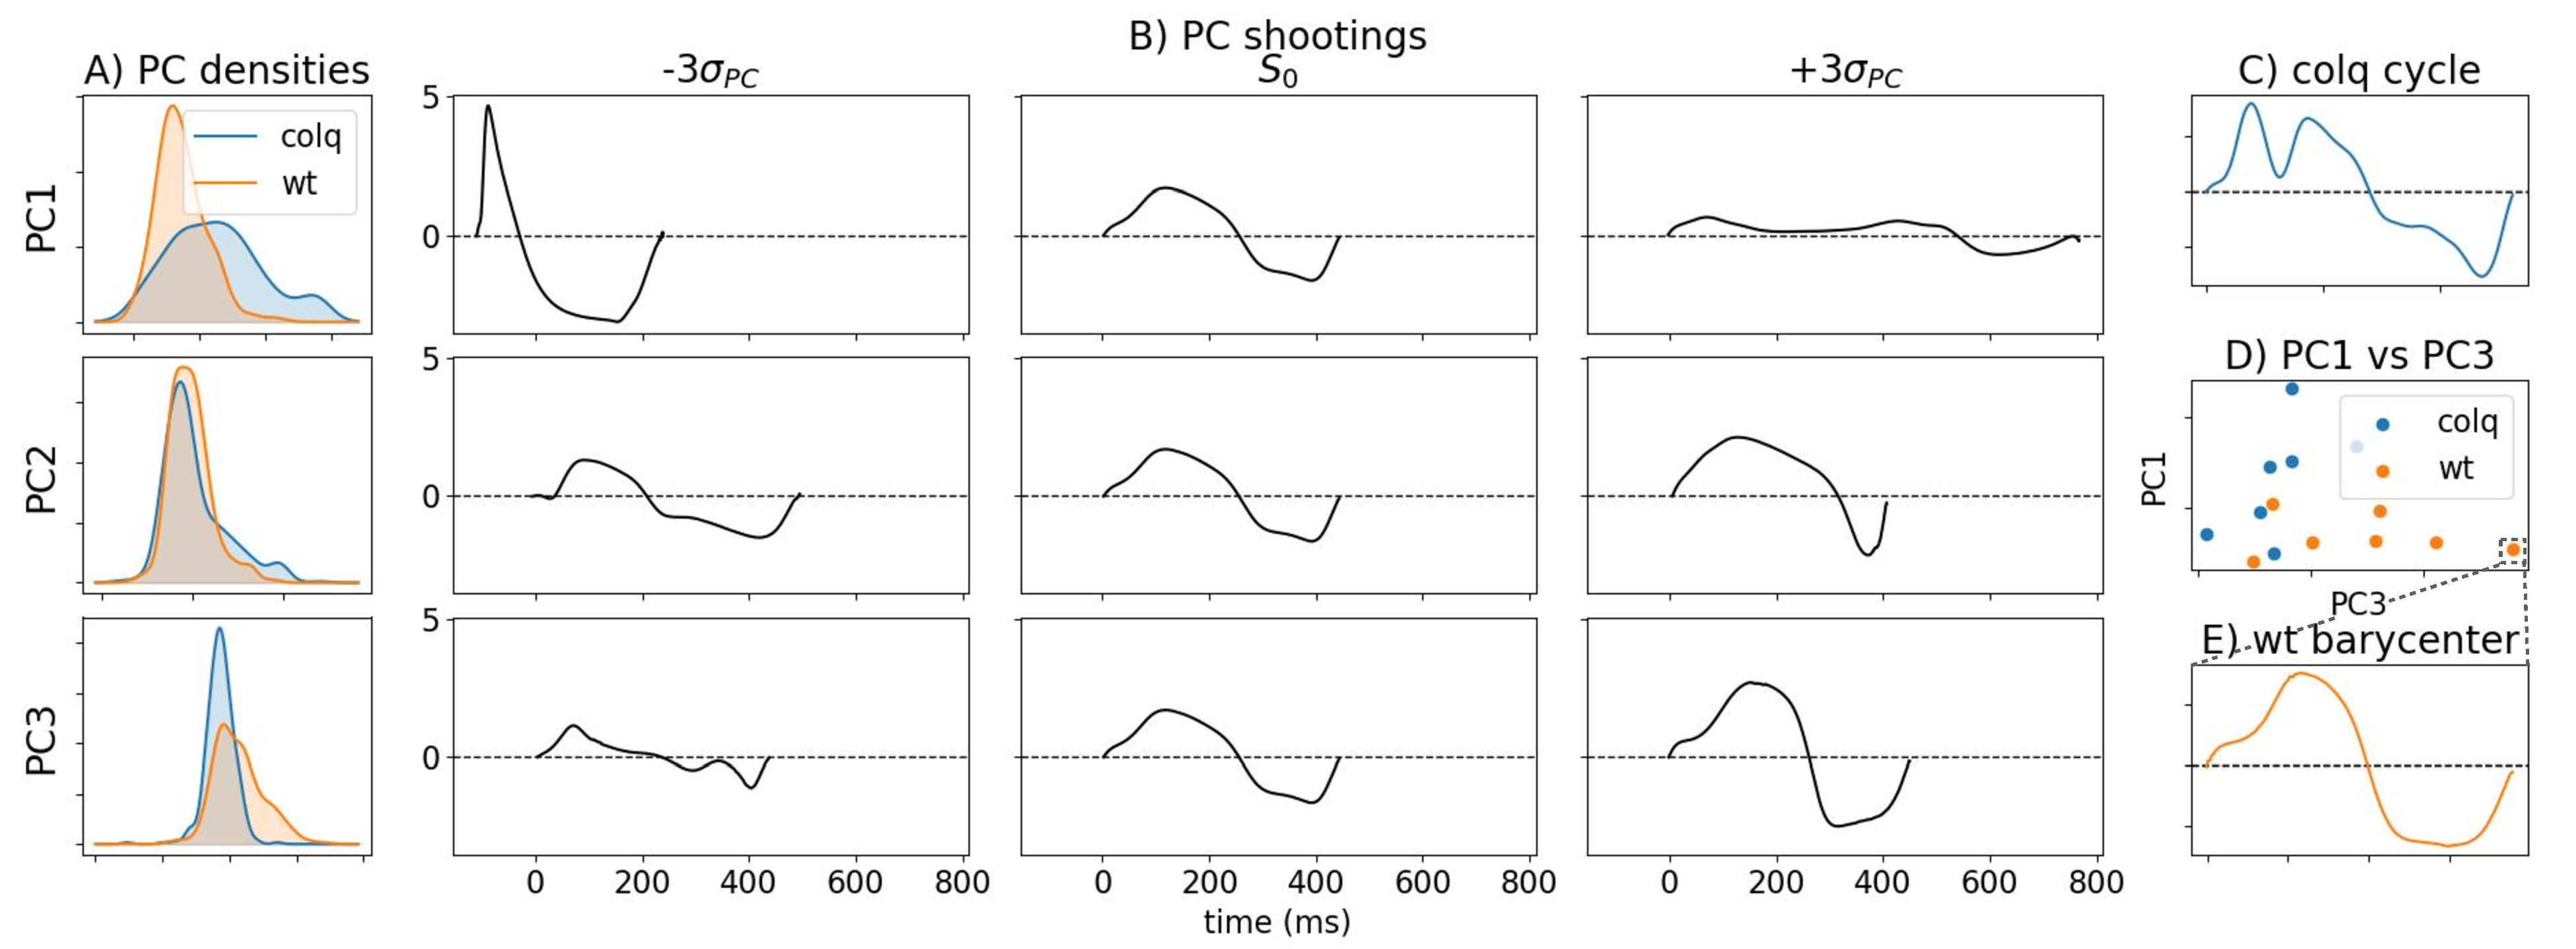
\includegraphics[width=0.95\linewidth]{"./pictures/exp_1_bis.pdf"}
  \vspace{-1.5em}
  \caption{Analysis of the three principal components (PC) related to the respiratory cycles of the mouse before exposure.
  In Figure A), the densities of each genotype according to each PC are displayed. In Figure B), the deformations of the reference graph $S_0$ along each PC are given. In Figure D), the graph of reference $S^j$, also called barycenter, related to each mouse, is displayed according to their coordinates on PC1 and PC3. In Figure C) et E), illustrations of respiratory cycles related to mice coming from the \textbf{wt} and \textbf{colq} group are displayed.  }
  \label{fig:exp_1_PCA}
  %\vspace{-1em}
\end{figure*}

\begin{figure*}[t]
  \centering
  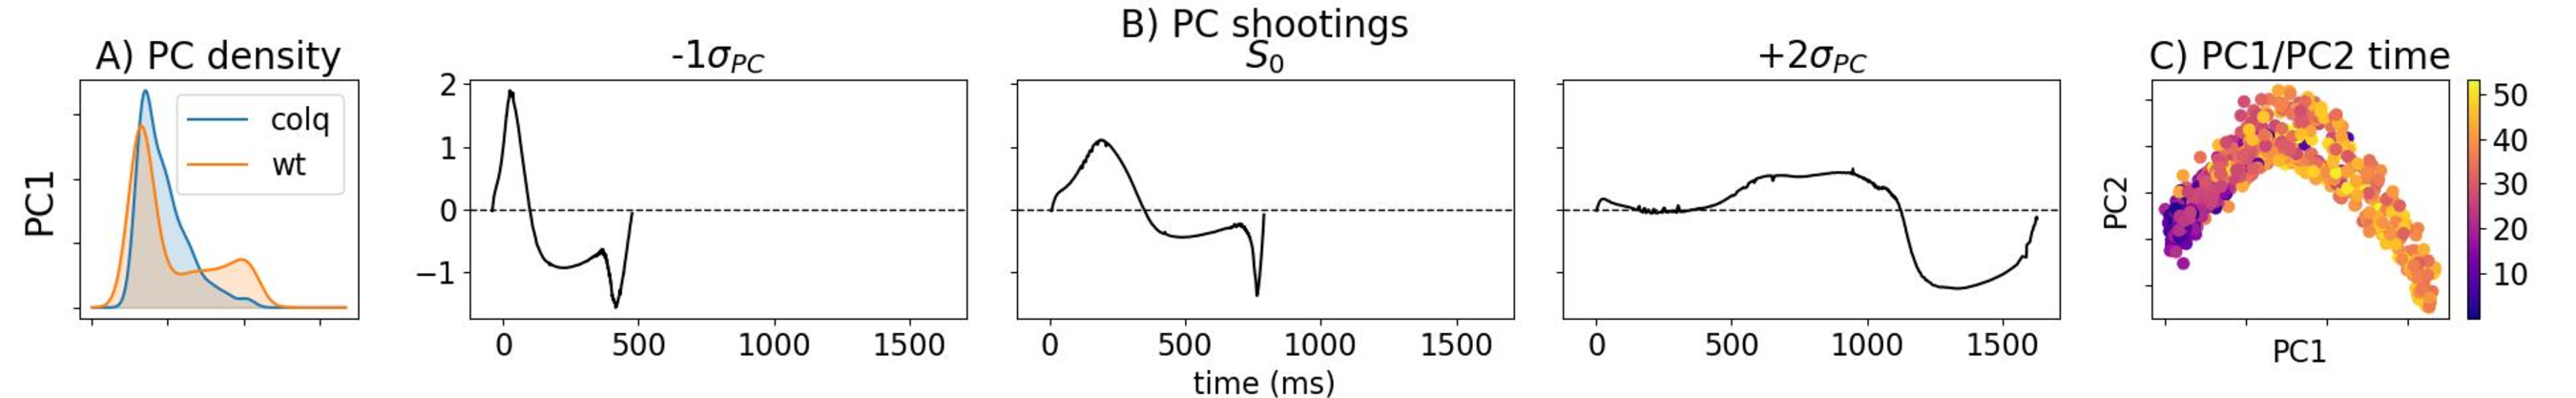
\includegraphics[width=0.95\linewidth]{"./pictures/exp_2.pdf"}
  \vspace{-1em}
  \caption{Analysis of the first Principal Component (PC1) related to the respiratory cycles of the mouse 
  before and after exposure. In Figure A), the densities of each genotype according are displayed. In Figure B), the deformations of the reference graph $S_0$ PC1 is given. In Figure C), respiratory cycles displayed with respect to time and according to their coordinates on PC1 and PC2}
  \label{fig:exp_2_PCA}
  \vspace{-1.5em}
\end{figure*}

This experiment highlights the \textit{interpretability} of TS-LDDMM for studying the inter-individual variability in a clinical dataset.
We consider a time series dataset recording the evolution of the respiratory airflow of mice exposed 
to an irritant molecule altering respiratory functions \cite{nervo2019respiratory}. The dataset is divided into two groups, one 
composed of 7 control mice (\textbf{wt}) and the other of 7 mice (\textbf{colq}) deficient in an enzyme 
involved in the control of respiration. For each mouse, the respiratory airflow was recorded for 
15 to 20 minutes before exposure to the irritant molecule and then for 35 to 40 minutes. A complete 
description of the dataset is given in the \Cref{appendix:mouse_dataset}.
By comparing the shape of individual respiratory cycles (inspiration + expiration, see \Cref{fig:exp_1_PCA}-C)), 
we show that TS-LDDMM features can encode genotype distinctive breathing behaviors and their evolution 
after exposure to the irritant molecule. 

We first compare breathing behaviors before exposure.
Solving \eqref{eq:general_optimization_problem}, we derive the reference respiratory cycle's graph $S_0$ and the TS-LDDMM features representations 
$(\alpha_j)_{j\in[N_1]}$ related to $N_1=700$ respiratory cycles extracted according 
to the procedure \cite{germain2023unsupervised}.
Then, we perform a kernel PCA on the initial velocity field $\left(v_0(\alpha_j,S_0)\right)_{j\in[N_1]}\in \msv^{N_1}$ defined in \eqref{eq:def_v0}.
In \Cref{fig:exp_1_PCA}, we focus on the analysis of the three Principal Components (PC).

As observable from \Cref{fig:exp_1_PCA}-B), principal components refer to different types of deformations. 
By interpreting \Cref{fig:exp_1_PCA}-B): Only PC1 accounts for time warping, PC2 expresses the trade-off between inspiration and expiration duration, and PC3 corresponds to a change in signal amplitude.
 Compared to \textbf{wt} mice, the distribution of \textbf{colq} mice 
TS-LDMMM feature representation along the PC1 axis has a heavy tail and the associated deformation (+3 $\sigma_{\text{PC}}$) 
shows an inspiration with two peaks. As illustrated in \Cref{fig:exp_1_PCA}-A), such respiratory cycles are preponderant
 with \textbf{colq} mice and may be caused by motor impairment due to their enzyme deficiency, \cite{germain2023unsupervised}.
  In addition, 
 the \textbf{colq} mice were smaller than the \textbf{wt} mice due to a delay in growth caused by their lack of an enzyme. 
 This difference can be seen on PC3 since the volumes of air (area under the curve) inspired and exhaled are
  smaller for the smaller mice. In correlation, the distribution of \textbf{wt} mice TS-LDDMM feature representations 
  along the PC3 axis have a heavy tail corresponding to large air volume as depicted by the deformation 
  (+3 $\sigma_{\text{PC}}$) in \Cref{fig:exp_1_PCA}-B). Finally, \Cref{fig:exp_1_PCA}-D) shows that PC1 and PC3 capture the main differences between
   the two groups as their respective reference graphs $S^j$ are located in different parts of the space. 
%In Figure \Cref{fig:exp_1_PCA}, we display coordinates densities per genotype and PC.

We perform a second experiment to analyze the evolution of breathing behaviors when mice are exposed to the irritant 
molecule. We follow the same procedure as before. However, we take $N_2=1400$ with 25\% (resp. 75\%) 
before (resp. after) exposure. In \Cref{fig:exp_2_PCA}, we focus on the first principal component PC since
it encodes the effect of the irritant molecule as depicted in \Cref{fig:exp_2_PCA}-C) (the exposure occurs at 20 minutes).
\Cref{fig:exp_2_PCA}-B) shows that the deformation (+3 $\sigma_{\text{PC}}$) leads to longer respiratory cycles that include pauses,
as observed in \cite{germain2023unsupervised}. As well, \Cref{fig:exp_2_PCA}-A) shows that TS-LDDMM features distributions are less spread 
out for \textbf{colq} mice compared to \textbf{wt} mice. Indeed, the irritant molecule inhibits the action of the 
deficient enzyme, \textbf{wt} mice strongly react to the irritant molecule, whereas \textbf{colq} mice are better 
adapted due to their deficiency.
%Secondly, we compare breathing behaviors before and after exposure to observe the impact of the irritant molecule.
% We follow the same procedure as for before exposure, but we take $N_2=1400$ respiratory cycles extracted according 
% to the procedure CITE....
% In \Cref{fig:exp_2_PCA}, we focus on the first Principal Component (PC) since it encodes the effect of the irritant molecule as demonstrated on Figure \ref{fig:exp_2_PCA}-C) (exposure at time 20).
% We observe on \Cref{fig:exp_2_PCA}-B) that after exposure the mouse have longuer breath such that the expiration is longuer than inspiration.
%  Moreover, we deduce from Figure \ref{fig:exp_2_PCA}-A) that \textbf{colq} are more constant in their breath compared to \textbf{wt} after exposure.
%
% In Figure REF, we 
% also display the reference respiratory cycle S0 and its deformations in the principal component directions.
%  Additionally, we learn each mouse's reference respiratory cycle and represent them in the first and third PC coordinates system in Figure REF. 



\subsection{Quantitative performances of the TS-LDDMM representation in classification}
Combined with a Support Vector Classifier (SVC) \cite{hsu2003practical}, TS-LDDMM representation can be used for 
classification tasks using the kernel associated with the initial velocity space $\msv$.
We compare TS-LDDMM-SVC classification performances with another SVC using representation 
learned with T-loss \cite{franceschi2019unsupervised}, an unsupervised deep learning feature 
representation method for time series. We also include fully supervised methods in deep learning 
-ResNet, CNN \cite{ismail2019deep}- and machine learning: Catch22 \cite{lubba2019catch22}, Rocket
\cite{dempster2020rocket}, Dynamic Time Wrapping k-Nearest Neighbors (DTW-kNN) 
\cite{muller2007dynamic}. Methods are compared using f1-score on several shape-based UCR/UEA datasets 
\cite{dau2019ucr,bagnall2018uea} introduced in \Cref{appendix:classification_dataset}. All implementation details are given 
in \Cref{appendix:classification_implementation}.
\Cref{table:classification} presents the reuslts. TS-LDDMM-SVC consistently outperforms the other unsupervised methods. It is ranked 1,3,4,3 for all methods combined, 
demonstrating its competitiveness as an unsupervised method on time series dataset homogeneous regarding shape.
%TS-LDDMM representation can be used in a Support Vector Classifier (SVC) \cite{hsu2003practical} using the kernel of the space of initial velocity $\msv$.
%We compare its capacity of representation to an SVC using T-Loss representation \cite{franceschi2019unsupervised}, which is an unsupervised representation deep learning method for time series,
%and to others fully supervised methods using deep learning -ResNet, CNN \cite{ismail2019deep}- or not: Catch22 \cite{lubba2019catch22}, Rocket \cite{dempster2020rocket}, Dynamic Time Wrapping \cite{muller2007dynamic} k-Nearest Neighbors (DTW-kNN).
%These methods are compared using f1-score on several datasets introduced in \Cref{appendix:classification_dataset}. All details of implementations are given in \Cref{appendix:classification_implementation}.
%TS-LDDMM-SVC is always ranked 2 or 3 behind a fully supervised method, demonstrating its competitiveness as an unsupervised method.
%The more homogeneous the shapes in the dataset are, the better TS-LDDMM-SVC performs.


\begin{table}[t]
  \vspace{-0.5em}
  \caption{Classification results in f1-score (U: unsupervised, S: supervised, DL: deep learning, ML: machine learning). \textbf{x} best unsupervised method, \underline{x} best supervised method.}
  \resizebox{\linewidth}{!}{%
  \begin{tabular}{lllrrrr}
    \toprule
     &  &  & ArrowHead & ECG200 & GunPoint & NATOPS \\
    \midrule
    \multirow[m]{3}{*}{U} & \multirow[t]{3}{*}{} & TS-LDDMM-SVC & \textbf{0.84} & \textbf{0.82} & \textbf{0.94} & \textbf{0.93} \\
     &  & T-loss-SVC & 0.57 & 0.76 & 0.82 & 0.88 \\
     &  & DTW-kNN & 0.70 & 0.75 & 0.91 & 0.88 \\
    \cline{1-7} 
    \multirow[m]{5}{*}{S} & \multirow[m]{2}{*}{DL} & CNN & 0.70 & 0.79 & 0.85 & \underline{0.96} \\
     &  & ResNet & 0.77 & 0.87 & 0.97 & 0.95 \\
    \cline{2-7}
     & \multirow[m]{2}{*}{ML} & Catch22 & 0.73 & 0.81 & 0.96 & 0.89 \\
     &  & Rocket & \underline{0.81} & \underline{0.91} & \underline{1.00} & 0.88 \\
    \bottomrule
    \end{tabular}
    \label{table:classification}
  %
}
\vspace{-2em}
  \end{table}
\section{Conclusion}
In this paper, we propose a feature representation method, TS-LDDMM, designed for 
shape comparison in homogeneous time series datasets. We show on a real dataset 
its ability to study, with high interpretability, the inter-individual shape 
variability. As an unsupervised approach, it is user-friendly and enables knowledge 
transfer for different supervised tasks such as classification. Although TS-LDDMM 
is already competitive for classification, its performances can be leveraged on 
more heterogeneous datasets using a hierarchical clustering extension, which is relagated for future work. 

%\section{Societal impact}
%This paper presents work whose goal is to advance the field of Machine Learning. There are many potential societal consequences of our work, none which we feel must be specifically highlighted here.
% \section{Acknowledgements}

%The TS-LDDMM feature representation proposed in this paper enables us to study the inter-individual variability of shapes in a time series dataset with high interpretability.
%Its unsupervised aspect is user-friendly and enables knowledge transfer for different supervised tasks such as classification.
%Although the method is already competitive,
% its capacity can be leveraged on more heterogeneous datasets using a hierarchical clustering extension.
% This is relegated to future works.

%Applying NF or CNF to our
 %  framework with high dimensional time series is relagated for future works.

% \begin{figure}[ht]
% \vskip 0.2in
% \begin{center}
% \centerline{\includegraphics[width=\columnwidth]{icml_numpapers}}
% \caption{Historical locations and number of accepted papers for International
% Machine Learning Conferences (ICML 1993 -- ICML 2008) and International
% Workshops on Machine Learning (ML 1988 -- ML 1992). At the time this figure was
% produced, the number of accepted papers for ICML 2008 was unknown and instead
% estimated.}
% \label{icml-historical}
% \end{center}
% \vskip -0.2in
% \end{figure}


% \begin{algorithm}[tb]
%    \caption{Bubble Sort}
%    \label{alg:example}
% \begin{algorithmic}
%    \STATE {\bfseries Input:} data $x_i$, size $m$
%    \REPEAT
%    \STATE Initialize $noChange = true$.
%    \FOR{$i=1$ {\bfseries to} $m-1$}
%    \IF{$x_i > x_{i+1}$}
%    \STATE Swap $x_i$ and $x_{i+1}$
%    \STATE $noChange = false$
%    \ENDIF
%    \ENDFOR
%    \UNTIL{$noChange$ is $true$}
% \end{algorithmic}
% \end{algorithm}








\begin{ack}
  \sam{tofill }
  Use unnumbered first level headings for the acknowledgments. All acknowledgments
  go at the end of the paper before the list of references. Moreover, you are required to declare
  funding (financial activities supporting the submitted work) and competing interests (related financial activities outside the submitted work).
  More information about this disclosure can be found at: \url{https://neurips.cc/Conferences/2024/PaperInformation/FundingDisclosure}.
  
  
  Do {\bf not} include this section in the anonymized submission, only in the final paper. You can use the \texttt{ack} environment provided in the style file to automatically hide this section in the anonymized submission.
  \end{ack}

\bibliographystyle{plain}
\bibliography{ref.bib}

\newpage




%%%%%%%%%%%%%%%%%%%%%%%%%%%%%%%%%%%%%%%%%%%%%%%%%%%%%%%%%%%%

\appendix





%%%%%%%%%%%%%%%%%%%%%%%%%%%%%%%%%%%%%%%%%%%%%%%%%%%%%%%%%%%%%%%%%%%%%%%%%%%%%%%
%%%%%%%%%%%%%%%%%%%%%%%%%%%%%%%%%%%%%%%%%%%%%%%%%%%%%%%%%%%%%%%%%%%%%%%%%%%%%%%
% APPENDIX
%%%%%%%%%%%%%%%%%%%%%%%%%%%%%%%%%%%%%%%%%%%%%%%%%%%%%%%%%%%%%%%%%%%%%%%%%%%%%%%
%%%%%%%%%%%%%%%%%%%%%%%%%%%%%%%%%%%%%%%%%%%%%%%%%%%%%%%%%%%%%%%%%%%%%%%%%%%%%%%



\section{Proofs}
\label{appendix:proofs}
Denote by $\msg(s)\triangleq \{ (t,s(t)): \eqsp t\in \msi \} $ the graph of a time series $s: \msi \to \Rset^d$ and $ \phi.\msg(s)\triangleq\{ \phi(t,s(t)): \eqsp t\in \msi\} $ the action of  $\phi\in \mcd(\Rset^{d+1}) $ on $\msg(s)$.
\begin{theorem}
    \label{theorem:representation_proof}
Let $s:  \msj \to \Rset^d  $ and $\mathbf{s}_0: \msi\to \Rset^d $ be two continuously differentiable time seriess with $\msi,\msj$ two intervals of $\Rset$.
 There exist $f\in \rmC^1(\Rset^{d+1},\Rset^d)$ and $\gamma\in  \mcd(\Rset) $ such that $\gamma(\msi)=\msj $ and $\Phi_f\in \mcd(\Rset^{d+1})$,
 \begin{equation}% TO add more detail on functionnal space
    \msg(s)= \Pi_{\gamma,f}.\msg(\mathbf{s}_0),\eqsp \Pi_{\gamma,f}=\Psi_\gamma\circ\Phi_f.
 \end{equation}
 Moreover, for any $\bar{f}\in \rmC^1(\Rset^{d+1},\Rset^d)$ and $\bar{\gamma}\in  \mcd(\Rset) $, there exists a continously differentiable time series $\bar{s}$ such that 
 $\msg(\bar{s})= \Pi_{\bar{\gamma},\bar{f}}.\msg(\mathbf{s}_0)$
\end{theorem}
%\sam{preuve todo, classement des variétés à bord, donne un homeomorphisme sur la restriction}
\begin{proof}
  Let $s:  \msj \to \Rset^d  $ and $\mathbf{s}_0: \msi\to \Rset^d $ be two continuously differentiable time seriess with $\msi=(a,b),\msj=(\alpha,\beta)$ two intervals of $\Rset$.
  By setting $\gamma: t\in \Rset \mapsto (\beta-\alpha)(t-a)/(b-a)+\alpha\in \Rset $, we have $ \gamma(\msi)=\msj$ and $\gamma \in \mcd(\Rset) $.
   By defining $f:(t,x)\in\Rset^{d+1}\mapsto x-\mathbf{s}_0(t)+s\circ \gamma(t) $, the map $\Phi_f\in \mcd(\Rset^{d+1})$,
    indeed, its inverse is $\Phi_f^{-1}:(t,x)\in\Rset^{d+1}\mapsto (t,x+\mathbf{s}_0(t)-s(t)) $ and is continuously differentiable.
     Moreover, we have $\Pi_{\gamma,f}.\msg(\mathbf{s}_0)=\{(\gamma(t),s\circ \gamma(t)):\eqsp t\in\msi \}=\msg(s) $.

    

    Let $\bar{f}\in \rmC^0(\Rset^{d+1},\Rset^d)$, $\bar{\gamma}\in  \mcd(\Rset) $ and $\mathbf{s}_0\in \rmC^0(\msi,\Rset^d)$ with $\msi$ an interval of $\Rset$.
    We have :
    \begin{align}
      \Pi_{\gamma,f}.\msg(\mathbf{s}_0)&=\{(\gamma(t),f(t,\mathbf{s}_0(t))),\eqsp t\in \msi \} \\
      &\label{eq:proof1_last_eq}=\{(t,f\left(\gamma^{-1}(t),\mathbf{s}_0(\gamma^{-1}(t))\right),\eqsp t\in \gamma(\msi) \} \eqsp .
    \end{align}
    By defining $\bar{s}:t\in \gamma(\msi)\to f\left(\gamma^{-1}(t),\mathbf{s}_0(\gamma^{-1}(t))\right) $, we have $\bar{s}\in \rmC^0(\gamma(\msi), \Rset^d) $ by composition of continuous functions
    and $ \msg(\bar{s})= \Pi_{\gamma,f}.\msg(\mathbf{s}_0)$ by \eqref{eq:proof1_last_eq}, which concludes the proof.
\end{proof}
\begin{lemma}
  If we denote by $\msv$ the RKHS associated with the kernel $K_{\msg}$, then for any vector field $v$ generated by \eqref{eq:integration} with $v_0$ satisfying \eqref{eq:def_v0},
   there exist $\gamma \in \msd(\Rset) $ and $f\in \rmC^1(\Rset^{d+1},\Rset^d)$ such that $\phi^v=\Psi_\gamma\circ\Phi_f $.
\end{lemma}
\begin{proof}
  Let $v$ be a vector field generated by \eqref{eq:integration} with $v_0$ satisfying \eqref{eq:def_v0}.
 We remark that the first coordinate of the velocity field $v_\tau$ denoted by $v_\tau^{\text{time}}$ only depends on the time variable $t$ for any $\tau\in[0,1]$.
 Thus, when computing the first coordinate of the deformation $\phi^v$, denoted by $\gamma$, we integrate \eqref{eq:LDDMM_dynamic} with $v_\tau$ replaced by $v_\tau^{\text{time}}$,
  thus $\gamma$ is independant of the variable $x$. Moreover, $\gamma\in \mcd(\Rset)$ since a Gaussian kernel induced an Hilbert space $\msv$ satisfying $|f|_V\leq |f|_\infty+ |\dd f|_\infty  $ for any $f\in \msv$ by \citep[Theorem 9]{glaunes2005transport}.
  For the same reason, we have $\phi^v\in \mcd(\Rset^{d+1})$, and thus its last coordinates denoted by $f$ belongs to $\rmC^1(\Rset^{d+1},\Rset^d)$, and by construction $\phi^v=\Psi_\gamma\circ\Phi_f $.
\end{proof}




\section{Oriented varifold}

\label{appendix:varifold}
In this section, we introduce the \textit{oriented varifold} associated with curves.
For further readings on curves and surfaces representation as varifolds, readers can refer to \cite{kaltenmark2017general,charon2013varifold}. 
We associate to $\gamma\in \rmC^1((a,b),\Rset^{d+1})$ an \textit{oriented varifold} $\mu_\gamma$, i.e. a distribution on the space $\Rset^{d+1}\times \mathbb{S}^{d}$ defined as follows, for any smooth test function $\omega :\Rset^{d+1}\times \mathbb{S}^{d}\to \Rset  $,
\begin{equation}
  \mathbb{E}_{Y\sim \mu_\gamma}\left[\omega(Y)\right]=\mu_\gamma(\omega)=\int_a^b \omega\left(\gamma(t),\frac{\dot{\gamma}(t)}{|\dot{\gamma}(t)|}\right)|\dot{\gamma}(t)|\dd t \eqsp .
\end{equation}
Denoting by $\msw$ the space of smooth test function, we have that $\mu_\gamma $ belongs to its dual $\msw^*$.
 Thus, a distance on $\msw^*$ is sufficient to set a distance on oriented varifolds associated to curve and thus on $\rmC^1((a,b),\Rset^{d+1})$ by the identification $\gamma\to \mu_\gamma $.
Remark that in (TS-LDDMM), $\gamma$ should be the parametrization of a time series' graph $\msg(s)$, i.e. $\gamma: t\in \msi \to (t,s(t))\in\Rset^{d+1} $ denoting by $s:\msi \to \Rset^d$ the time series.
However, in practice, we work with discrete objects.
 That is why, we set $W$ as an RKHS to use its representation theorem.
 More specifically \citep[Proposition 2 \& 4]{kaltenmark2017general} encourages us to consider a kernel $k:(\Rset^{d+1} \times \mathbb{S}^d)^2\to \Rset$ such that there exist two positive and continuously differentiable kernels $k_{\pos}$ and $k_{\dir}$, 
 such that for any $(x,\overrightarrow{u}),(y,\overrightarrow{v}) \in (\Rset^{d+1} \times \mathbb{S}^d)^2$
 \begin{equation}
     k((x,\overrightarrow{u}),(y,\overrightarrow{v})) = k_{\pos}(x,y)k_{\dir}(\overrightarrow{u},\overrightarrow{v}) \eqsp,
   \end{equation}
 with moreover $k_\dir>0$ and $ k_\pos$ which admits an RKHS $\msw_\pos$ dense in the space of continous function on $\Rset^{d+1}$ vanishing at infinite \cite{carmeli2010vector}.

Given such a kernel $k:(\Rset^{d+1} \times \mathbb{S}^d)^2\to \Rset$
verifying \citep[Proposition 2 \& 4]{kaltenmark2017general}, we have that for any $(x,v)\in \Rset^{d+1}\times \mathbb{S}^{d}$, $\delta_{(x,\overrightarrow{v})}$ belongs to $\msw^*$ as a distribution and that the dual metric $\langle\cdot,\cdot \rangle_{\msw^*} $ satisfies for any $(x_1,v_1),(x_2,v_2)\in \left(\Rset^{d+1}\times \mathbb{S}^{d}\right)^2$,
\begin{equation}
  \langle\delta_{(x_1,\overrightarrow{v}_1)},\delta_{(x_2,\overrightarrow{v}_2)} \rangle_{\msw^*} =k((x_1,\overrightarrow{v}_1),(x_2,\overrightarrow{v}_2)) \eqsp .
\end{equation}
Thus, given two sets of triplets $X=(l_i,x_i,\overrightarrow{v}_i)_{i\in[T_0-1]}\in (\Rset\times \Rset^{d+1}\times \mathbb{S}^d)^{T_0-1},Y=(l_i',y_i,\overrightarrow{w}_i)_{i\in[T_1]}\in (\Rset\times \Rset^{d+1}\times \mathbb{S}^d)^{T_1-1}$ and denoting by 
\begin{equation}
  \label{eq:def_mu_X}
  \mu_X=\sum_{i=1}^{T_0} l_i \delta_{(x_i,\overrightarrow{v}_i)},\mu_Y=\sum_{i=1}^{T_1} l_i' \delta_{(y_i,\overrightarrow{w}_i)} \eqsp,
\end{equation}
 we have,
\begin{equation}
   |\mu_X-\mu_Y |_{\msw^*}^2 = \sum_{i,j = 1}^{T_0-1}l_i k((x_i,\overrightarrow{v_i}),(x_i,\overrightarrow{v_i}^0))l_j - 2 \sum_{i=1}^{T_0-1}\sum_{j=1}^{T_1-1}l_i k((x_i,\overrightarrow{v_i}),(y_i,\overrightarrow{w_i}))l_j' + \sum_{i,j = 1}^{T_1-1}l_i' k((y_i,\overrightarrow{w_i}),(y_i,\overrightarrow{w_i}))l_j' \eqsp.
\end{equation}
Then, using the identification $X\to \mu_X, Y\to \mu_Y$, we can define a distance on sets of triplets as $d_{\msw^*,3}(X,Y)=|\mu_X-\mu_Y|_{\msw^*}^2$.

Now, we aim to discretize the oriented varifold $\mu_\msg $ related to a time series' graph $\msg(s)$ by using a set of triplets.
This is carried out by using a discretized version of $\msg(s) $, i.e. $\tilde{\msg}=(g_i=(t_i,s(t_i)))_{i\in[T]}\in(\Rset^{d+1})^T$, in the following way: 
For any  $i\in[T-1]$, denoting the center and length of the $i^{th}$ segment $[g_i,g_{i+1}]$ by
$c_i = (g_i + g_{i+1})/2$, $l_i = \| g_{i+1}-g_{i}\|$, and the unit norm vector of direction $\overrightarrow{g_i g_{i+1}}$ by
 $\overrightarrow{v_i} = (g_{i+1}-g_{i})/l_i$, we define the set of triplets $X(\tilde{\msg})=(l_i,c_i,\overrightarrow{v_i})_{i\in[T-1]}$ and its related oriented varifold $\mu_{X(\tilde{\msg})}= \sum_{i=1}^{T-1}l_i \delta_{c_i,\overrightarrow{v_i}}$ as in \eqref{eq:def_mu_X}.
 This is a valid discretization of the oriented varifold $\mu_\msg$ according to \citep[Proposition 1]{kaltenmark2017general}: $\mu_{X(\tilde{\msg})}$ converges towards $\mu_\msg$ as the size of the descretization mesh $\sup_{i\in[T-1]} |t_{i+1}-t_i| $ converges to 0.

 Finally, we define a distance on discretized time series' graphs $\tilde{\msg}_1,\tilde{\msg}_2$ as $d_{\msw^*}(\tilde{\msg}_1,\tilde{\msg}_2)=d_{\msw^*,3}(X(\tilde{\msg}_1),X(\tilde{\msg}_2)) $.


\subsection{Varifold kernels}
\label{appendix:kernel_implementation}
Denote the one-dimensional Gaussian kernel by $K_\sigma^{(a)}(x,y)=\exp(-|x-y|^2/\sigma)$ for any $(x,y)\in (\Rset^a)^2$, $a\in \Nset$ and $\sigma>0$.
In the implementation, we use the following kernels, for any $((t_1,x_1),(t_2,x_2))\in (\Rset^{d+1})^2, ((w_1,v_1),(w_2,v_2))\in (\mathbb{S}^{d})^2 $,
\begin{equation}
  k_{\pos}(x,y)=K_{\sigma_{\pos,t}}^{(1)}(t_1,t_2)K_{\sigma_{\pos,x}}^{(d)}(x_1,x_2),\quad k_{\pos}(x,y)=K_{\sigma_{\dir,t}}^{(1)}(w_1,w_2)K_{\sigma_{\dir,x}}^{(d)}(v_1,v_2)\eqsp ,
\end{equation}
where $\sigma_{\pos,t}, \sigma_{\pos,x}, \sigma_{\dir,t}, \sigma_{\dir,x}>0 $ are hyperparameters.
 In practice, we select $\sigma_{\pos,x}\approx \sigma_{\dir,x} \approx 1$ when the times series are centered and normalized. Otherwise we select $\sigma_{\pos,x}\approx \sigma_{\dir,x} \approx \bar{\sigma}_{s}$ with $\bar{\sigma}_{s}$ the average standard deviation of the time series.
  We choose $\sigma_{\pos,t}\approx \sigma_{\dir,t} = m f_e$ with $f_e$ the sampling frequency of the time series and $m\in [5]$ an integer depending on the time change between the starting and the target time series graph.
  The more significant the time change, the higher $m$ should be. The intuition comes from the fact that the width $\sigma_{\pos,t}, \sigma_{\dir,t}$ rules the time windows used to perform the comparison, and $\sigma_{\pos,x}, \sigma_{\dir,x}$ affects the space window.
   The size of the windows should be selected depending on the variations in the data.

\section{Tuning the hyperparameters of the TS-LDDMM kernel given in \eqref{eq:kernel_TAS}}
\label{appendix:kernel_TS_LDDMM}
The parameter $\sigma_{T,0}$ should be chosen \textit{large} compared the sampling frequency $f_e$ and compared to average standard deviation $\bar{\sigma}_s$ of the time series, e.g $\sigma_{T,0}=100$ as $\bar{\sigma}_s\approx f_e\approx  1 $.
It makes the time transformation smoother. If $\sigma_{T,0}$ is too small, for instance, $\sigma_{T,0}=f_e $, the effect of the time deformation is too localized, and there are not enough samples to make it visible.

The parameter $\sigma_{T,1}$ should be of the same order as $f_e$: two different points in time can have various space transformations.
 $\sigma_x$ should be of the same order of $\bar{\sigma}_s$: two points with a big difference regarding space compared to $\bar{\sigma}_s$ can have very different space transformations.

 We take $c_0\approx 10 c_1 $, we want to encourage time transformation before space transformation. We take $(c_0,c_1)=(1,0.1)$ in all experiments.


\section{Numerical details}
A report of all the hyperparameters selected is given in \Cref{appendix:table:set_up_exp_practical}.
\subsection{Optimization details of \eqref{eq:general_optimization_problem}}
\label{appendix:optimizers_details}
\paragraph{Initialization}
At the initialization of \eqref{eq:general_optimization_problem}, all the momentums parameter are set to $0$ and the graph of reference is set to the graph of a time series in the dataset having a mediane samples size.

\paragraph{Gradient descent.}
The chosen gradient descent method is "adabelief" \cite{zhuang2020adabelief} implemented in the library OPTAX\footnote{https://optax.readthedocs.io/en/latest/}.
There are two main parameters in the gradient descent: the number of steps nb\_steps, and the maximum value of step size $\eta_M$.
The stepsize has a particular scheduling: 
\begin{itemize}
  \item Warmup period on $0.1 \times$ nb\_steps steps: the stepsize increases linearly from $0$ to $\eta_M$. The goal is to learn progressively the parameters.
   If the stepsize is too large at the start, smaller steps at the end can't make up for the mistakes made at the beginning. 
  \item Fine tuning periode on $ 0.9  \times$ nb\_steps : the stepsize decreases from $\eta_M$ to $0$ with a cosine decay implemented in the OPTAX scheduler,
   i.e. the decreasing factor as the form $0.5  (1 + \cos(\pi  t/T))$. 
\end{itemize}
The sharper the deformations, the larger the number of steps and the maximum value of step size should be selected.
We suggest nb\_steps=300, $\eta_M=0.1 $ for small deformations and nb\_steps=800, $\eta_M=0.3 $ for big ones (time dilation with a factor $\lambda\geq 2$).

\subsection{Synthetic experiments}
\label{appendix:numerics_synthetic}
For any deformations generation in both experiments (well-specified and misspecified), we take $\sigma_{T,0},\sigma_{T,1},\sigma_x=(100,1,1)$ and $c_0,c_1=(1,0.1)$ for the kernel $K_\msg$
and $\sigma_{\pos,t}, \sigma_{\pos,t}, \sigma_{\dir,t}, \sigma_{\dir,x}=(2,1,2,0.6) $ for the varifold kernels $k_\pos,k_\dir$ related to the loss $\scrl$.

In both experiments, we have nb\_steps=300 abd $\eta_M=0.1$.

\subsection{Mouse experiments}
The number of steps is larger in the second experiment (before/after injection) because the deformations are sharper.

\subsection{Classification experiments}
\label{appendix:classification_implementation}

We defined a default parametrization for all classifiers. 

For classifiers: \href{https://www.aeon-toolkit.org/en/stable/api_reference/auto_generated/aeon.classification.deep_learning.CNNClassifier.html#aeon.classification.deep_learning.CNNClassifier}{CNN}, 
\href{https://www.aeon-toolkit.org/en/stable/api_reference/auto_generated/aeon.networks.ResNetNetwork.html#aeon.networks.ResNetNetwork}{ResNet}, 
\href{https://www.aeon-toolkit.org/en/stable/api_reference/auto_generated/aeon.classification.feature_based.Catch22Classifier.html#aeon.classification.feature_based.Catch22Classifier}{Catch22}, 
\href{https://www.aeon-toolkit.org/en/stable/api_reference/auto_generated/aeon.classification.distance_based.KNeighborsTimeSeriesClassifier.html#aeon.classification.distance_based.KNeighborsTimeSeriesClassifier}{DTW-KNN}, 
\href{https://www.aeon-toolkit.org/en/stable/api_reference/auto_generated/aeon.classification.convolution_based.RocketClassifier.html#aeon.classification.convolution_based.RocketClassifier}{Rocket}
we used the aeon\footnote{https://www.aeon-toolkit.org/en/stable/index.html} implementations with their default settings. 

For Tloss-SVC we used the implementation provided on github\footnote{https://github.com/mqwfrog/ULTS} 
with the following parameters for learning representations: batch\_size: 10, channels: 40, depth: 10, nb\_steps: 200, in\_channels: 1, 
kernel\_size: 3, lr: 0.001, nb\_random\_samples: 10, negative\_penalty: 1, out\_channels: 320, reduced\_size: 160. 
We used the Support Vector Classifier (\href{https://scikit-learn.org/stable/modules/generated/sklearn.svm.SVC.html#sklearn.svm.SVC}{SVC})
from scikit-learn with thee regularization term C: 1. Others parameters are set to default.

For TS-LDDMMM-SVC, all kernels' parameters et optimizer parameter are presented in \Cref{appendix:table:set_up_exp_practical}.
As well, we used the Support Vector Classifier from scikit-learn with thee regularization term C: 1. Others parameters are set to default.


 \begin{table}[hbt!]
  \caption{Parameters used in all the experiments.
   For synthetic data, $K_\msg$ refers to the kernel used in the generation, which is the same for the estimation only in the well-specified case. $\bar{l}$ refers to the average time series length and $N_d$ refers to the number of dimensions.}
  \centering
  \begin{tabular}{lllll}

            \toprule 
            objects & Optimizer &$k_\pos,k_\dir$ & $K_\msg $ \\
            \midrule
            Parameter & (nb\_steps,$\eta_M$) &$(\sigma_{\pos,t}, \sigma_{\pos,t}, \sigma_{\dir,t}, \sigma_{\dir,x})$ & $(c_0,c_1,\sigma_{T,0},\sigma_{T,1},\sigma_x)$ \\
            \midrule
            Synthetic data well-specified &(300,0.1) &$(2,1,2,0.6)$& $(1,0.1,100,1,1)$   \\
            Synthetic data misspecified  & (300,0.1)  & $ (2,1,2,0.6)$ &$(1,0.1,100,1,1)$  \\
            Mouse before injection  & (400,0.3)  & $ (2,1,2,0.6)$ &$(1,0.1,100,1,1)$  \\
            Mouse before/after injection  & (800,0.3)  & $ (5,1,5,0.6)$ &$(1,0.1,150,1,1)$  \\
            classification  & (400,0.1)  & $(\max(2,0.03\bar{l}),N_d,\max(2,0.03\bar{l}),0.6)$  & $(1,0.1,0.33\bar{l},1,N_d)$  \\

            \bottomrule
          \end{tabular}
        \label{appendix:table:set_up_exp_practical}
    \end{table}
\section{Mouse respiratory dataset}

\begin{figure}
  \centering
  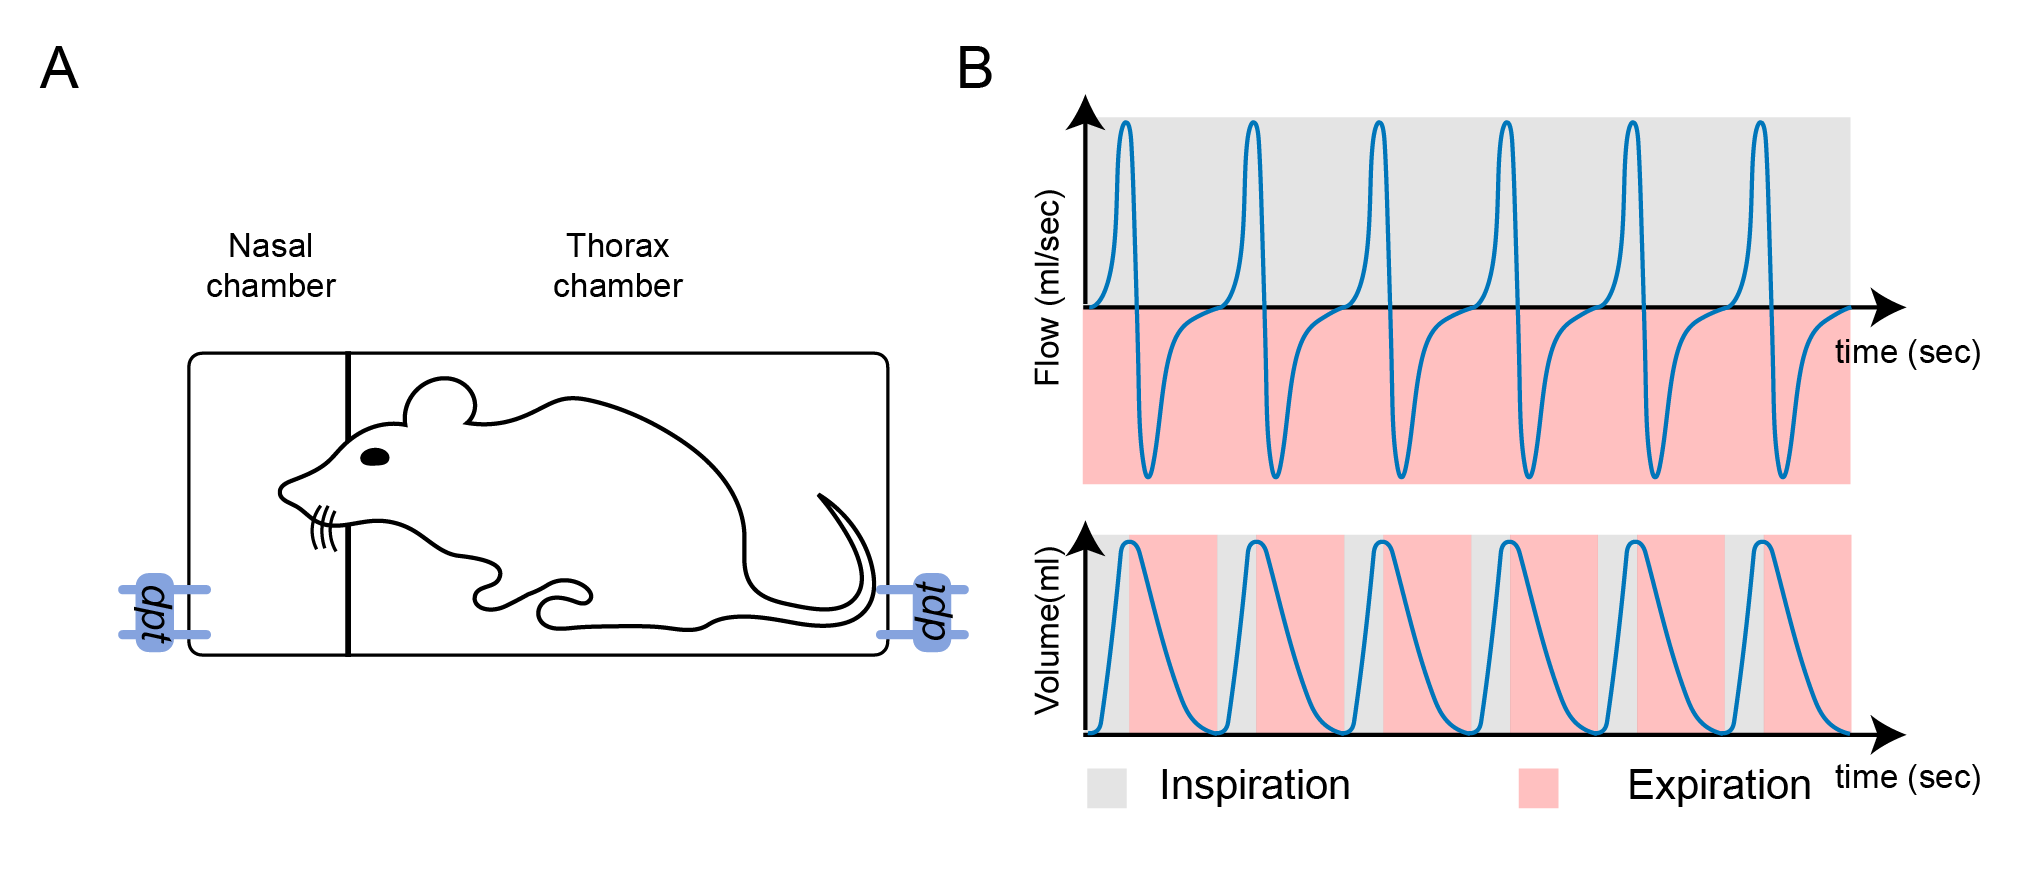
\includegraphics[width = \linewidth]{pictures/mice_exp.png}
  \caption{A: Illustration of a double-chamber plethysmograph. The term \textit{dpt} stands for differential 
  pressure transducer which measures the pressure in each compartment, the pressure then being converted to flow. 
  B: Nasal airflow (top) and lung volume (bottom). During inspiration, airflow is positive (grey) and during
  expiration, airflow is negative (pink).}
  \label{fig:mice_exp}
\end{figure}

\label{appendix:mouse_dataset}
Ventilation is a simple physiological function that ensures a vital supply of oxygen and the elimination of CO2. 
Acetylcholine (Ach) is a neurotransmitter that plays an important role in muscular activity, notably for breathing. 
Indeed, muscle contraction information passes from the brain to the muscle through the nervous system. Achs are located 
in synapses of the nervous system (central and peripheral) and skeletal muscles. They ensure the information transmission 
from nerve to nerve. However, the transmission cannot end without the hydrolysis of Ach by the enzyme Acetylcholinesterase 
(AchE), allowing nerves to return to their resting state. Inhibition of (AchE) with, for instance, nerve gas, pesticide, 
or drug intoxication leads to respiratory arrests. 

The dataset comes from the experiment \cite{nervo2019respiratory}, where they studied the consequences of partial 
deficits in AChE and AChE inhibition on mice respiration. AchE inhibition was induced with an 
irritant molecule called physostigmine (an AchE inhibitor). Mice nasal airflows were sampled at 
2000Hz with a Double Chamber plethysmograph \cite{hoymann2012lung}, as depicted in \Cref{fig:mice_exp}-A). The flow is expressed in 
$ml.s^{-1}$; it has a positive value during inspiration and a negative value expiration \Cref{fig:mice_exp}-B). 
Among the mice population, we selected 7 control mice (\textbf{wt}) and 7 ColQ mice (\textbf{colq}), which do not have 
AChE anchoring in muscles and some tissues. 
As described in \cite{nervo2019respiratory}, mice experiments were as follows:
\begin{enumerate}
  \item The mouse is placed in a DCP for 15 or 20 min to serve as an internal control.
  \item The mouse is removed from the DCP and injected with physostigmine.
  \item The mouse is placed back into the DCP, and its nasal flow is recorded for 35 or 40 min.
\end{enumerate}

Respiratory cycles were extracted following procedure \cite{germain2023unsupervised}. We removed 
respiratory cycles whose duration exceeds 1 second; the average respiratory cycle duration is 
300 ms. We randomly sampled 10 respiratory cycles per minute and mouse. It leads to a dataset of 
12,732 (time, genotype)-annotated respiratory cycles. 

\section{Classification: Comparison with shape analysis methods}

In this section, we compare classification performances of TS-LDDMM with other state-of-the-art methods coming from shape analysis on 15 shape-based datasets of time-series.

\paragraph{Methods} We compare TS-LDDMM with a method from function~\cite{wu2024shape}

\paragraph{Protocole}

\begin{table}[hbt!]
  \centering
  \resizebox{\columnwidth}{!}{%
  \begin{tabular}{llrrrr}
    \toprule
     & \textbf{Dataset} & \textbf{Shape-FPCA (2024)} & \textbf{TCLR (2024)} & \textbf{LDDMM (2008)} & \textbf{TS-LDDMM (ours)} \\
    \midrule
    \multirow[c]{7}{*}{Univariate} & ArrowHead & 0.18 & 0.75 & \underline{0.84} & \textbf{0.91} \\
     & BME & 0.16 & \underline{1.00} & 0.82 & \textbf{1.00} \\
     & ECG200 & 0.40 & 0.67 & \textbf{0.81} & \underline{0.79} \\
     & FacesUCR & 0.08 & \underline{0.73} & 0.69 & \textbf{0.86} \\
     & GunPoint & 0.93 & \underline{0.97} & 0.83 & \textbf{1.00} \\
     & PhalangesOutlinesCorrect & 0.39 & \textbf{0.63} & \underline{0.53} & 0.52 \\
     & Trace & 0.55 & \underline{1.00} & 0.46 & \textbf{1.00} \\
    \cline{1-6}
    \multirow[c]{8}{*}{Multivariate} & ArticularyWordRecognition & -- & -- & \underline{0.98} & \textbf{1.00} \\
     & Cricket & -- & -- & \underline{0.77} & \textbf{0.93} \\
     & ERing & -- & -- & \underline{0.95} & \textbf{0.98} \\
     & Handwriting & -- & -- & \underline{0.22} & \textbf{0.44} \\
     & Libras & -- & -- & \underline{0.56} & \textbf{0.60} \\
     & NATOPS & -- & -- & \underline{0.82} & \textbf{0.82} \\
     & RacketSports & -- & -- & \textbf{0.83} & \underline{0.79} \\
     & UWaveGestureLibrary & -- & -- & \underline{0.72} & \textbf{0.81} \\
    \bottomrule
    \end{tabular}
    %
  }
    
\end{table}


\section{Classification datasets}
\label{appendix:classification_dataset}
We selected 15 shape-based datasets (7 univariates and 8 multivariates) from the from the University of East Anglia (UEA) and the University of California Riverside (UCR) Time Series Classification Repository\footnote{https://timeseriesclassification.com} \cite{dau2019ucr,bagnall2018uea}. All datasets were downloaded with the python package aeon\footnote{https://www.aeon-toolkit.org/en/stable/}. Essential datasets information are summarized in \Cref{appendix:table:datasets} and further can be found in \cite{dau2019ucr,bagnall2018uea}.

\begin{table}[hbt!]
  \centering
  \caption{UCR/UEA shape-based time series datasets for classification.}
  \resizebox{\columnwidth}{!}{%
  \begin{tabular}{lllllll}
    \toprule
    & \textbf{Dataset} &  \textbf{Size} & \textbf{Lengh} & \textbf{Number of classes} & \textbf{Number of dimensions} & \textbf{Type} \\
    \midrule
    \multirow[c]{7}{*}{Univariate} &  ArrowHead & 211 & 251 & 3 & 1 & IMAGE \\
    & BME & 180 & 128 & 3 & 1 & SIMULATED \\
    & ECG200 & 200 & 96 & 2 & 1 & ECG \\
    & FacesUCR & 2250 & 131 & 14 & 1 & IMAGE \\
    & GunPoint & 200 & 150 & 2 & 1 & MOTION \\
    & PhalangesOutlinesCorrect & 2658 & 80 & 2 & 1 & IMAGE \\
    & Trace & 200 & 275 & 4 & 1 & SENSOR \\
    \cline{1-7}
    \multirow[c]{8}{*}{Multivariate}& ArticularyWordRecognition & 575 & 144 & 25 & 9 & SENSOR \\
    & Cricket & 180 & 1197 & 12 & 6 & MOTION \\
    & ERing & 60 & 65 & 6 & 4 & SENSOR \\
    & Handwriting & 1000 & 152 & 26 & 3 & MOTION \\
    & Libras & 360 & 45 & 15 & 2 & VIDEO \\ 
    & NATOPS & 360 & 51 & 6 & 24 & MOTION \\
    & RacketSports & 303 & 30 & 4 & 6 & SENSOR \\
    & UWaveGestureLibrary & 240 & 315 & 8 &3 & SENSOR \\
    \bottomrule
  \end{tabular}
  %
  }
  \label{appendix:table:datasets}
\end{table}




    
%  [11:35, 31/01/2024] Thibaut Germain: avant/après :
%  [11:35, 31/01/2024] Thibaut Germain: Kv = VFTSGaussKernel(1,0.1,150,1,1)
%  Kl = TSGaussGaussKernel(5,1,5,0.6)
%  dataloss = VarifoldLoss(Kl)
%  schedule = warmup_cosine_decay_schedule(0,0.3,80,800,0)
%  [11:35, 31/01/2024] Thibaut Germain: avant :
%  [11:35, 31/01/2024] Thibaut Germain: Kv = VFTSGaussKernel(1,0.1,100,1,1)
%  Kl = TSGaussGaussKernel(2,1,2,0.6)
%  dataloss = VarifoldLoss(Kl)
%  schedule = warmup_cosine_decay_schedule(0,0.3,40,400,0)
% Let $s$ be a time series and $\msg(\tilde{s}) = (g_i)_{i \in [n]}$ be its discretized graph.
%  The graph $\msg(s)$ can be approximated as 
% the union of piecewise linear segments between time-consecutive samples, 
% and we associate to the approximated graph the oriented varifold:

% \begin{equation}
%   \mu_{\msg(\tilde{s})} : w \in \msw \mapsto \sum_{i=1}^{n-1} l_i\delta_{(c_i,\overrightarrow{v_i})}(w)
% \end{equation}
% where $\msw$ is a set of real valued test functions defined on $\Rset^{d+1} \times \mathbb{S}^d$, 
% $\delta_{(c_i,\overrightarrow{v_i})}(w) = w(c_i,\overrightarrow{v_i})$ is a Dirac delta function, 
% $c_i = (g_i + g_{i+1})/2$ (resp. $v_i = \| g_{i+1}-g_{i}\|$) is the center (resp. length) of the $i^{th}$ segment, 
% and $\overrightarrow{v_i} = (g_{i+1}-g_{i})/l_i$ is the unit norm vector of direction $\overrightarrow{g_i g_{i+1}}$.

% Assuming that the test functions' space $\msw$ is the RKHS associated with a $C^1$ positive definite kernel $k$ 
% that verifies \citep[Proposition 2 \& 4]{kaltenmark2017general}, the oriented varifold belongs to the dual space $\msw^*$. Additionally, 
% we can define a distance $d_{\msw^*}$ between signals' graph sample sets, which, thanks to the kernel reproducing property,
% has an explicit formulation: 


% \section{Continuous normalizing flows}
% %Modeling Continuous Stochastic Processes with Dynamic Normalizing Flows time series generative
% CONTUNYIYS NORMALIZING FLOW bofbof
% Here, we present the framework of Continuous Normalizing Flows (CNF) and show how LDDMM can be seen as a particular case.
% \cite{salman2018deep} was already inspired from the work of shape analysis to present deep diffeomorphic normalizing flows.
% Discussion with Alain :
% Given a time-dependant vector field $v:[0,1]\times \Rset^{d'} \to \Rset^{d'} $, the integration of this vector field gives a flow $ \phi:[0,1]\times \Rset^{d'} \to \Rset^{d'}$, defined via the ordinary differential equation (ODE),
% \begin{equation}
%   \frac{\dd }{\dd \tau}\phi_\tau(x)=v(\tau,\phi_\tau(x)), \phi_0(x)=x \eqsp.
%  \end{equation}
% In \cite{chen2018neural}, they introduce Continous Normalizing flows for generative modeling.
%  By modeling $v=f_\theta$ is a neural networks and choosing a prior $X_0\sim\rho_0$ on the inital value, the law of $\phi_1(X_0)$ has the pullback density $\phi_1\# \rho_0$ and the parameter $\theta$ is optimized to maximize the log-likelihood of a given dataset $(y_i)_{i\in[N]}\in (\Rset^{d'})^N$ which is assumed to follow the law of $\phi_1(X_0)$.
% Instead of modeling the law of the end point $\phi_1(X_0) $, we can try to model the law of the whole path $(\phi_\tau(X_0))_{\tau\in[0,1]} $ having a density $p:[0,1]\times \Rset^d\to \Rset_{>0}$ such that $p_1=q, p_0=\rho_0$ where $q$ is the empirical distribution in the dataset, as proposed in \cite{lipman2022flow}.
% In so doing, the problem is ill-posed since $p_t$ can be whatever as soon as $0<t<1$, that is why we try to constraint the learned velocity field $v=f_\theta$ such that the path law $p$ is tractable.
% One way of doing it is to look for geodesics \eqref{eq:geodesics_original} as proposed in LDDMM, it corresponds to the case where $q=\sum_{i=1}^N \delta_{y_i}/N$ and $\rho_0=\sum_{i=1}^N \delta_{x_i}/N$ are empirical distribution and $y_i=\phi^v_1(x_i) $ for a given velocity field $v$.

% The goal is to target $\nu\in \mathcal{P}(\rmC^0([0,1]\times \Rset^d, \Rset^d)) $ by generating randomness on a initial value $x \sim \delta_x$
%  and by integrating a velocity field $v_\theta \in \msw \subset \rmC^0([0,1]\times \Rset^d, \Rset^d)$: 
%  \begin{equation}
%   \frac{\dd h}{\dd \tau}=v_\theta(\tau,h(\tau,x)), h(0,x)=x \eqsp,
%  \end{equation}
%  denoting by $\mu$ the law of $(h(\tau,x))_{\tau \in [0,1]}$. 

%%%%%%%%%%%%%%%%%%%%%%%%%%%%%%%%%%%%%%%%%%%%%%%%%%%%%%%%%%%%%%%%%%%%%%%%%%%%%%%
%%%%%%%%%%%%%%%%%%%%%%%%%%%%%%%%%%%%%%%%%%%%%%%%%%%%%%%%%%%%%%%%%%%%%%%%%%%%%%%


% \subsection{TTS}
% To circumvant this issue, we propose two methods :
%       \begin{enumerate}
%         \item \label{enum:first_method} [Time And Space (TAS)] Using a specific form of the RKHS's kernel in LDDMM, to stick to the classical shape analysis framework.
%         \item \label{enum:second_method} [Time Then Space (TTS)] Tackling the time axis and space axis separetely in the transformation.
%          This distangles time and space variability in the patterns, increasing the interpretability of the representation.
%           Although the related optimization is more complex than method \ref{enum:first_method}, the results is more robust to the choice of hyper-parameter related to the RKHS's kernel.
%       \end{enumerate}
%        In the following, we present both methods to highlights their pro and cons.


% As described in \Cref{section:optimization}, the method (TAS) learns $\Pi_{\gamma,f}$ directly, while (TTS) find the temporal reparametrisation $\Phi_f$ then the space transformation $\Psi_\gamma$.
%     % If we define a diffeomorpshim $\Phi_\gamma$ as $(\gamma,\Id_d) $, we have $\Phi_\gamma.G(s) =G(s).\gamma^{-1}$.
%     %  To increase the variability, we allow some deformations on the graph of the time series after being reparametrized in time, which allow us to recover every possible time seriess.
%     % Remark that, $G(\mathbf{s}_0\circ \psi^{-1})=\{(t,\mathbf{s}_0\circ \psi^{-1}(t)), t\in \msj \}= \{(\psi(t),\mathbf{s}_0(t)) ,\eqsp t\in \msi \}  $.
%     % [The action of the diffeomorpshim group 
%     % \begin{align}
%     %     &\mcd_*=\mcd(\Rset,\Rset)\times \{\phi\in \mcd(\Rset^{d+1},\Rset^{d+1}): \\
%     %     &\phi(t,x)=(t,f(t,x)),
%     %      (t,x)\in \Rset \times \Rset^{d}, f \in C^0(\Rset^{d+1}, \Rset^d) \} 
%     % \end{align}
%     % on the space of time series graph $\{G^{(a,b)}(s), s\in C^0((a,b), \Rset), (a,b)\in \Rset_+^2, a<b  \}$
%     % is homogene.]
%      %In the next section we define a metric and a norm on this space in order to find a representation $(\phi,\psi)$ with a minimal norm, and we show in (...) how to recover a proxy.
%      \paragraph{The representation as the solution of an optimization}
%      By \Cref{theorem:representation}, for any $\mathbf{s}_0\in C^0(\msi,\Rset^d)$, we can find $ F=(\gamma_j,f_j)_{j\in[N]}$ such that $\msg(s^j)=\Pi_{\gamma_j,f_j}.\msg(\mathbf{s}_0)$ for any $j\in[N]$.
%      However, to get a meaningfull representation and to tackle the unicity problem, we should optimize the choice of $\mathbf{s}_0 $ and $F$, formally speaking, denoting by $R(\cdot) $ a regularization norm on $\mcd(\Rset^{d+1})$ and $L$ a loss on sets which will be specify later, we aim to solve
%      \begin{equation}
%       \label{eq:minimization}
%       \underset{\mathbf{s_0},(\gamma_j,f_j)_{j\in[N]}}{ \argmin} \sum_{j=1}^N \lambda R(\Pi_{\gamma_j,f_j})+ L(\msg(s^j),\Pi_{\gamma_j,f_j}.\msg(\mathbf{s}_0)) \eqsp ,
%     \end{equation} 
%     where $\lambda>0$ is a penalization factor related to $L$ to relax the condition $\msg(s^j)=\Pi_{\gamma_j,f_j}.\msg(\mathbf{s}_0)$.

%     In practice, as already proposed in shape analysis, we perform an alternative minimization between $\mathbf{s_0}$ and $(\gamma_j,f_j)_j$.
%     The optimization on $(\gamma_j,f_j)_j$ is parrallelisable, for each couple $(\mathbf{s}_0,s^j)$, we should learn diffemorphisms of minimal norm satisfying a condition. 
%     To this end, we adapt the geodesic shooting method using LDDMM presented in \cite{durrleman2013sparse} to our special case.
%       Before to describe how to optimize the whole in \Cref{section:optimization}, we introduce LDDMM in the next section to specify the norm on diffemorphisms.

% \paragraph{Kernel choices}
% As depicted on figure (mettre ref), we can not use any kernel $K$ to apply the previous methodology to learn deformations on time series' graphs.

% In the following, we expose two choice of RKHS's kernel which answers this issue : (TAS) and (TTS).
%  We rely on the Gaussian kernel, denoting by $K_\sigma^{(a)}(x,y)=\exp(-|x-y|^2/\sigma)$ for any $(x,y)\in (\Rset^a)^2$, $a\in \Nset$ and $\sigma>0$.
% To apply (TAS) in LDDMM with $d'=d+1$, we use the following anisotropic Gaussian kernel  :
% \begin{align}
%   \label{eq:kernel_TAS}
%   &K_{\text{TAS}}((t,x),(t',x'))=\begin{pmatrix}
%     c_0K & 0 \\
%     0 & c_1 D 
%     \end{pmatrix} \eqsp , \\
%     &D=K_{\sigma_{T,1}}^{(1)}(t,t')K_{\sigma_x}^{(d)}(x,x') \Idd\eqsp,K=K_{\sigma_{T,0}}^{(1)}(t,t') \eqsp,
% \end{align}
% parametrized by the widths $\sigma_{T,0},\sigma_{T,1},\sigma_x>0$ and the constants $c_0,c_1>0$.
%  If we use this kernel, by considering \eqref{eq:specific_form}, we remark that the first coordinate of the velocity field $v_\tau$ only depends on the time variable $t$.
%   It implies that the final deformation will have the form $\phi^v=(\gamma,f) $ with  $f\in C^1(\Rset^{d+1},\Rset^d) $, and $\gamma\in \mcd(\Rset)$
%   since the first coordinate follows a LDDMM-ODE \eqref{eq:LDDMM_dynamic}.


% To apply (TTS), we use LDDMM on the time axis with $d'=1$ by taking $K_{\text{TTS}}^{\text{time}}=K_{\sigma_{T,0}}^{(1)}$, then on the space axis with $d'=d$ by choosing
% $K_{\text{TTS}}^{\text{space}}=K_{\sigma_{T,1}}^{(1)}\times K_{\sigma_x}^{(d)} $ where the widths are the same than in \eqref{eq:kernel_TAS}. The alternate optimization will be more detailed in \Cref{section:optimization}.



% This document was modified from the file originally made available by
% Pat Langley and Andrea Danyluk for ICML-2K. This version was created
% by Iain Murray in 2018, and modified by Alexandre Bouchard in
% 2019 and 2021 and by Csaba Szepesvari, Gang Niu and Sivan Sabato in 2022.
% Modified again in 2023 by Sivan Sabato and Jonathan Scarlett.
% Previous contributors include Dan Roy, Lise Getoor and Tobias
% Scheffer, which was slightly modified from the 2010 version by
% Thorsten Joachims & Johannes Fuernkranz, slightly modified from the
% 2009 version by Kiri Wagstaff and Sam Roweis's 2008 version, which is
% slightly modified from Prasad Tadepalli's 2007 version which is a
% lightly changed version of the previous year's version by Andrew
% Moore, which was in turn edited from those of Kristian Kersting and
% Codrina Lauth. Alex Smola contributed to the algorithmic style files.

\section*{NeurIPS Paper Checklist}




\begin{enumerate}

\item {\bf Claims}
    \item[] Question: Do the main claims made in the abstract and introduction accurately reflect the paper's contributions and scope?
    \item[] Answer: \answerYes{} % Replace by \answerYes{}, \answerNo{}, or \answerNA{}.
    \item[] Justification: Each claim in the introduction is referring to the part where it is tackled.
    \item[] Guidelines:
    \begin{itemize}
        \item The answer NA means that the abstract and introduction do not include the claims made in the paper.
        \item The abstract and/or introduction should clearly state the claims made, including the contributions made in the paper and important assumptions and limitations. A No or NA answer to this question will not be perceived well by the reviewers. 
        \item The claims made should match theoretical and experimental results, and reflect how much the results can be expected to generalize to other settings. 
        \item It is fine to include aspirational goals as motivation as long as it is clear that these goals are not attained by the paper. 
    \end{itemize}

\item {\bf Limitations}
    \item[] Question: Does the paper discuss the limitations of the work performed by the authors?
    \item[] Answer: \answerYes{} % Replace by \answerYes{}, \answerNo{}, or \answerNA{}.
    \item[] Justification: We have provided a special section for this purpose \Cref{sec:limitations}.
    \item[] Guidelines:
    \begin{itemize}
        \item The answer NA means that the paper has no limitation while the answer No means that the paper has limitations, but those are not discussed in the paper. 
        \item The authors are encouraged to create a separate "Limitations" section in their paper.
        \item The paper should point out any strong assumptions and how robust the results are to violations of these assumptions (e.g., independence assumptions, noiseless settings, model well-specification, asymptotic approximations only holding locally). The authors should reflect on how these assumptions might be violated in practice and what the implications would be.
        \item The authors should reflect on the scope of the claims made, e.g., if the approach was only tested on a few datasets or with a few runs. In general, empirical results often depend on implicit assumptions, which should be articulated.
        \item The authors should reflect on the factors that influence the performance of the approach. For example, a facial recognition algorithm may perform poorly when image resolution is low or images are taken in low lighting. Or a speech-to-text system might not be used reliably to provide closed captions for online lectures because it fails to handle technical jargon.
        \item The authors should discuss the computational efficiency of the proposed algorithms and how they scale with dataset size.
        \item If applicable, the authors should discuss possible limitations of their approach to address problems of privacy and fairness.
        \item While the authors might fear that complete honesty about limitations might be used by reviewers as grounds for rejection, a worse outcome might be that reviewers discover limitations that aren't acknowledged in the paper. The authors should use their best judgment and recognize that individual actions in favor of transparency play an important role in developing norms that preserve the integrity of the community. Reviewers will be specifically instructed to not penalize honesty concerning limitations.
    \end{itemize}

\item {\bf Theory Assumptions and Proofs}
    \item[] Question: For each theoretical result, does the paper provide the full set of assumptions and a complete (and correct) proof?
    \item[] Answer: \answerYes{} % Replace by \answerYes{}, \answerNo{}, or \answerNA{}.
    \item[] Justification: All the proofs are given in \Cref{appendix:proofs} and each proof state all its arguments in a logical order.
    \item[] Guidelines:
    \begin{itemize}
        \item The answer NA means that the paper does not include theoretical results. 
        \item All the theorems, formulas, and proofs in the paper should be numbered and cross-referenced.
        \item All assumptions should be clearly stated or referenced in the statement of any theorems.
        \item The proofs can either appear in the main paper or the supplemental material, but if they appear in the supplemental material, the authors are encouraged to provide a short proof sketch to provide intuition. 
        \item Inversely, any informal proof provided in the core of the paper should be complemented by formal proofs provided in appendix or supplemental material.
        \item Theorems and Lemmas that the proof relies upon should be properly referenced. 
    \end{itemize}

    \item {\bf Experimental Result Reproducibility}
    \item[] Question: Does the paper fully disclose all the information needed to reproduce the main experimental results of the paper to the extent that it affects the main claims and/or conclusions of the paper (regardless of whether the code and data are provided or not)?
    \item[] Answer: \answerYes{} % Replace by \answerYes{}, \answerNo{}, or \answerNA{}.
    \item[] Justification: The optimization methodology is described in \Cref{section:methodology} and all numerical details and protocol are given in \Cref{section:experiments} and in \Cref{appendix:classification_implementation}-\ref{appendix:optimizers_details}-\ref{appendix:numerics_synthetic}-\ref{appendix:identifiability}.
    \item[] Guidelines:
    \begin{itemize}
        \item The answer NA means that the paper does not include experiments.
        \item If the paper includes experiments, a No answer to this question will not be perceived well by the reviewers: Making the paper reproducible is important, regardless of whether the code and data are provided or not.
        \item If the contribution is a dataset and/or model, the authors should describe the steps taken to make their results reproducible or verifiable. 
        \item Depending on the contribution, reproducibility can be accomplished in various ways. For example, if the contribution is a novel architecture, describing the architecture fully might suffice, or if the contribution is a specific model and empirical evaluation, it may be necessary to either make it possible for others to replicate the model with the same dataset, or provide access to the model. In general. releasing code and data is often one good way to accomplish this, but reproducibility can also be provided via detailed instructions for how to replicate the results, access to a hosted model (e.g., in the case of a large language model), releasing of a model checkpoint, or other means that are appropriate to the research performed.
        \item While NeurIPS does not require releasing code, the conference does require all submissions to provide some reasonable avenue for reproducibility, which may depend on the nature of the contribution. For example
        \begin{enumerate}
            \item If the contribution is primarily a new algorithm, the paper should make it clear how to reproduce that algorithm.
            \item If the contribution is primarily a new model architecture, the paper should describe the architecture clearly and fully.
            \item If the contribution is a new model (e.g., a large language model), then there should either be a way to access this model for reproducing the results or a way to reproduce the model (e.g., with an open-source dataset or instructions for how to construct the dataset).
            \item We recognize that reproducibility may be tricky in some cases, in which case authors are welcome to describe the particular way they provide for reproducibility. In the case of closed-source models, it may be that access to the model is limited in some way (e.g., to registered users), but it should be possible for other researchers to have some path to reproducing or verifying the results.
        \end{enumerate}
    \end{itemize}


\item {\bf Open access to data and code}
    \item[] Question: Does the paper provide open access to the data and code, with sufficient instructions to faithfully reproduce the main experimental results, as described in supplemental material?
    \item[] Answer: \answerYes{} % Replace by \answerYes{}, \answerNo{}, or \answerNA{}.
    \item[] Justification: Synthetic data can be generated, benchmark data are publicly available (\Cref{appendix:classification_dataset}), but the mouse dataset is not.
     The code is provided as supplementary material and will be made publicly available if the paper is accepted.
    \item[] Guidelines:
    \begin{itemize}
        \item The answer NA means that paper does not include experiments requiring code.
        \item Please see the NeurIPS code and data submission guidelines (\url{https://nips.cc/public/guides/CodeSubmissionPolicy}) for more details.
        \item While we encourage the release of code and data, we understand that this might not be possible, so “No” is an acceptable answer. Papers cannot be rejected simply for not including code, unless this is central to the contribution (e.g., for a new open-source benchmark).
        \item The instructions should contain the exact command and environment needed to run to reproduce the results. See the NeurIPS code and data submission guidelines (\url{https://nips.cc/public/guides/CodeSubmissionPolicy}) for more details.
        \item The authors should provide instructions on data access and preparation, including how to access the raw data, preprocessed data, intermediate data, and generated data, etc.
        \item The authors should provide scripts to reproduce all experimental results for the new proposed method and baselines. If only a subset of experiments are reproducible, they should state which ones are omitted from the script and why.
        \item At submission time, to preserve anonymity, the authors should release anonymized versions (if applicable).
        \item Providing as much information as possible in supplemental material (appended to the paper) is recommended, but including URLs to data and code is permitted.
    \end{itemize}


\item {\bf Experimental Setting/Details}
    \item[] Question: Does the paper specify all the training and test details (e.g., data splits, hyperparameters, how they were chosen, type of optimizer, etc.) necessary to understand the results?
    \item[] Answer: \answerYes{} % Replace by \answerYes{}, \answerNo{}, or \answerNA{}.
    \item[] Justification: The experiments setting is clearly presented in \Cref{section:experiments} for the experiments on the mouse dataset. The full details of all experiments are presented in \Cref{appendix:classification_implementation}-\ref{appendix:optimizers_details}-\ref{appendix:numerics_synthetic}-\ref{appendix:identifiability}.
    \item[] Guidelines:
    \begin{itemize}
        \item The answer NA means that the paper does not include experiments.
        \item The experimental setting should be presented in the core of the paper to a level of detail that is necessary to appreciate the results and make sense of them.
        \item The full details can be provided either with the code, in appendix, or as supplemental material.
    \end{itemize}

\item {\bf Experiment Statistical Significance}
    \item[] Question: Does the paper report error bars suitably and correctly defined or other appropriate information about the statistical significance of the experiments?
    \item[] Answer: \answerNo{} % Replace by \answerYes{}, \answerNo{}, or \answerNA{}.
    \item[] Justification: Error bars are given for the synthetic experiments, but not for the real experiments due to limited computational budget.
     There is no randomness in the train/test split but there is randomness in the optimization method (Adabelief), but its impact is not significant on the results.
    \item[] Guidelines:
    \begin{itemize}
        \item The answer NA means that the paper does not include experiments.
        \item The authors should answer "Yes" if the results are accompanied by error bars, confidence intervals, or statistical significance tests, at least for the experiments that support the main claims of the paper.
        \item The factors of variability that the error bars are capturing should be clearly stated (for example, train/test split, initialization, random drawing of some parameter, or overall run with given experimental conditions).
        \item The method for calculating the error bars should be explained (closed form formula, call to a library function, bootstrap, etc.)
        \item The assumptions made should be given (e.g., Normally distributed errors).
        \item It should be clear whether the error bar is the standard deviation or the standard error of the mean.
        \item It is OK to report 1-sigma error bars, but one should state it. The authors should preferably report a 2-sigma error bar than state that they have a 96\% CI, if the hypothesis of Normality of errors is not verified.
        \item For asymmetric distributions, the authors should be careful not to show in tables or figures symmetric error bars that would yield results that are out of range (e.g. negative error rates).
        \item If error bars are reported in tables or plots, The authors should explain in the text how they were calculated and reference the corresponding figures or tables in the text.
    \end{itemize}

\item {\bf Experiments Compute Resources}
    \item[] Question: For each experiment, does the paper provide sufficient information on the computer resources (type of compute workers, memory, time of execution) needed to reproduce the experiments?
    \item[] Answer: \answerYes{} % Replace by \answerYes{}, \answerNo{}, or \answerNA{}.
    \item[] Justification: This is given at the beginning of \Cref{appendix:settings}.
    \item[] Guidelines:
    \begin{itemize}
        \item The answer NA means that the paper does not include experiments.
        \item The paper should indicate the type of compute workers CPU or GPU, internal cluster, or cloud provider, including relevant memory and storage.
        \item The paper should provide the amount of compute required for each of the individual experimental runs as well as estimate the total compute. 
        \item The paper should disclose whether the full research project required more compute than the experiments reported in the paper (e.g., preliminary or failed experiments that didn't make it into the paper). 
    \end{itemize}
    
\item {\bf Code Of Ethics}
    \item[] Question: Does the research conducted in the paper conform, in every respect, with the NeurIPS Code of Ethics \url{https://neurips.cc/public/EthicsGuidelines}?
    \item[] Answer: \answerYes{} % Replace by \answerYes{}, \answerNo{}, or \answerNA{}.
    \item[] Justification: Every authors are funded for their work and preserve research integrity.
    \item[] Guidelines:
    \begin{itemize}
        \item The answer NA means that the authors have not reviewed the NeurIPS Code of Ethics.
        \item If the authors answer No, they should explain the special circumstances that require a deviation from the Code of Ethics.
        \item The authors should make sure to preserve anonymity (e.g., if there is a special consideration due to laws or regulations in their jurisdiction).
    \end{itemize}


\item {\bf Broader Impacts}
    \item[] Question: Does the paper discuss both potential positive societal impacts and negative societal impacts of the work performed?
    \item[] Answer: \answerYes{} % Replace by \answerYes{}, \answerNo{}, or \answerNA{}.
    \item[] Justification: A special section is given on this subject \Cref{appendix:societal_impact}.
    \item[] Guidelines:
    \begin{itemize}
        \item The answer NA means that there is no societal impact of the work performed.
        \item If the authors answer NA or No, they should explain why their work has no societal impact or why the paper does not address societal impact.
        \item Examples of negative societal impacts include potential malicious or unintended uses (e.g., disinformation, generating fake profiles, surveillance), fairness considerations (e.g., deployment of technologies that could make decisions that unfairly impact specific groups), privacy considerations, and security considerations.
        \item The conference expects that many papers will be foundational research and not tied to particular applications, let alone deployments. However, if there is a direct path to any negative applications, the authors should point it out. For example, it is legitimate to point out that an improvement in the quality of generative models could be used to generate deepfakes for disinformation. On the other hand, it is not needed to point out that a generic algorithm for optimizing neural networks could enable people to train models that generate Deepfakes faster.
        \item The authors should consider possible harms that could arise when the technology is being used as intended and functioning correctly, harms that could arise when the technology is being used as intended but gives incorrect results, and harms following from (intentional or unintentional) misuse of the technology.
        \item If there are negative societal impacts, the authors could also discuss possible mitigation strategies (e.g., gated release of models, providing defenses in addition to attacks, mechanisms for monitoring misuse, mechanisms to monitor how a system learns from feedback over time, improving the efficiency and accessibility of ML).
    \end{itemize}
    
\item {\bf Safeguards}
    \item[] Question: Does the paper describe safeguards that have been put in place for responsible release of data or models that have a high risk for misuse (e.g., pretrained language models, image generators, or scraped datasets)?
    \item[] Answer: \answerNA{} % Replace by \answerYes{}, \answerNo{}, or \answerNA{}.
    \item[] Justification: There is no risk.
    \item[] Guidelines:
    \begin{itemize}
        \item The answer NA means that the paper poses no such risks.
        \item Released models that have a high risk for misuse or dual-use should be released with necessary safeguards to allow for controlled use of the model, for example by requiring that users adhere to usage guidelines or restrictions to access the model or implementing safety filters. 
        \item Datasets that have been scraped from the Internet could pose safety risks. The authors should describe how they avoided releasing unsafe images.
        \item We recognize that providing effective safeguards is challenging, and many papers do not require this, but we encourage authors to take this into account and make a best faith effort.
    \end{itemize}

\item {\bf Licenses for existing assets}
    \item[] Question: Are the creators or original owners of assets (e.g., code, data, models), used in the paper, properly credited and are the license and terms of use explicitly mentioned and properly respected?
    \item[] Answer: \answerYes{} % Replace by \answerYes{}, \answerNo{}, or \answerNA{}.
    \item[] Justification: All dataset and python library were cited when necessary.
    \item[] Guidelines:
    \begin{itemize}
        \item The answer NA means that the paper does not use existing assets.
        \item The authors should cite the original paper that produced the code package or dataset.
        \item The authors should state which version of the asset is used and, if possible, include a URL.
        \item The name of the license (e.g., CC-BY 4.0) should be included for each asset.
        \item For scraped data from a particular source (e.g., website), the copyright and terms of service of that source should be provided.
        \item If assets are released, the license, copyright information, and terms of use in the package should be provided. For popular datasets, \url{paperswithcode.com/datasets} has curated licenses for some datasets. Their licensing guide can help determine the license of a dataset.
        \item For existing datasets that are re-packaged, both the original license and the license of the derived asset (if it has changed) should be provided.
        \item If this information is not available online, the authors are encouraged to reach out to the asset's creators.
    \end{itemize}

\item {\bf New Assets}
    \item[] Question: Are new assets introduced in the paper well documented and is the documentation provided alongside the assets?
    \item[] Answer: \answerYes{} % Replace by \answerYes{}, \answerNo{}, or \answerNA{}.
    \item[] Justification: The mouse dataset is described in \Cref{appendix:mouse_dataset}.
    \item[] Guidelines:
    \begin{itemize}
        \item The answer NA means that the paper does not release new assets.
        \item Researchers should communicate the details of the dataset/code/model as part of their submissions via structured templates. This includes details about training, license, limitations, etc. 
        \item The paper should discuss whether and how consent was obtained from people whose asset is used.
        \item At submission time, remember to anonymize your assets (if applicable). You can either create an anonymized URL or include an anonymized zip file.
    \end{itemize}

\item {\bf Crowdsourcing and Research with Human Subjects}
    \item[] Question: For crowdsourcing experiments and research with human subjects, does the paper include the full text of instructions given to participants and screenshots, if applicable, as well as details about compensation (if any)? 
    \item[] Answer: \answerNA{} % Replace by \answerYes{}, \answerNo{}, or \answerNA{}.
    \item[] Justification: The paper does not involve crowdsourcing nor research with human subjects.
    \item[] Guidelines:
    \begin{itemize}
        \item The answer NA means that the paper does not involve crowdsourcing nor research with human subjects.
        \item Including this information in the supplemental material is fine, but if the main contribution of the paper involves human subjects, then as much detail as possible should be included in the main paper. 
        \item According to the NeurIPS Code of Ethics, workers involved in data collection, curation, or other labor should be paid at least the minimum wage in the country of the data collector. 
    \end{itemize}

\item {\bf Institutional Review Board (IRB) Approvals or Equivalent for Research with Human Subjects}
    \item[] Question: Does the paper describe potential risks incurred by study participants, whether such risks were disclosed to the subjects, and whether Institutional Review Board (IRB) approvals (or an equivalent approval/review based on the requirements of your country or institution) were obtained?
    \item[] Answer: \answerNA{} % Replace by \answerYes{}, \answerNo{}, or \answerNA{}.
    \item[] Justification: The paper does not involve crowdsourcing nor research with human subjects.
    \item[] Guidelines:
    \begin{itemize}
        \item The answer NA means that the paper does not involve crowdsourcing nor research with human subjects.
        \item Depending on the country in which research is conducted, IRB approval (or equivalent) may be required for any human subjects research. If you obtained IRB approval, you should clearly state this in the paper. 
        \item We recognize that the procedures for this may vary significantly between institutions and locations, and we expect authors to adhere to the NeurIPS Code of Ethics and the guidelines for their institution. 
        \item For initial submissions, do not include any information that would break anonymity (if applicable), such as the institution conducting the review.
    \end{itemize}

\end{enumerate}



\end{document}